\documentclass[BSc]{usydthesis}
\author{Ragib Zaman}
\title{Geometry and Topology of Toric Varieties}
\date{October 2013}
\numberwithin{equation}{chapter}
\theoremstyle{remark}
\newtheorem{Definition}[equation]{Definition}
\newtheorem{Theorem}[equation]{Theorem}
\newtheorem{Proposition}[equation]{Proposition}
\newtheorem{Lemma}[equation]{Lemma}
\newtheorem{Corollary}[equation]{Corollary}
\newtheorem{Remark}[equation]{Remark}
\newtheorem{Example}[equation]{Example}
\newcommand{\N}{\mathbb{N}}
\newcommand{\R}{\mathbb{R}}
\newcommand{\C}{\mathbb{C}}
\newcommand{\Z}{\mathbb{Z}}
\newcommand{\T}{\mathbb{T}}
\newcommand{\Proj}{\mathbb{P}}
\newcommand{\face}{\prec}
\newcommand{\V}{\vee}
\newcommand{\m}{\mathfrak{m}}
\newcommand{\M}{\operatorname{Mult}}
\DeclareMathOperator{\End}{End}
\DeclareMathOperator{\Hom}{Hom}
\DeclareMathOperator{\im}{im}
\DeclareMathOperator{\Cone}{Cone}
\DeclareMathOperator{\Spec}{Spec}
\newcommand{\map}[2]{\,{:}\,#1\!\longrightarrow\!#2}


\begin{document}  
\pagenumbering{roman}
\maketitle          % creates the title page
\tableofcontents    % creates the table of contents


\chapter*{Introduction} 
In this essay we study a special class of algebraic varieties called toric varieties. To each toric variety there is an associated arrangement of cones called a fan. Many geometric and topological properties of a toric variety are encoded in its fan's combinatorial and geometric data. Thus toric varieties present themselves with an alternate and effective way of studying them, as many problems about toric varieties can be reduced to more concrete statements about their fans. This makes them an ideal testing ground for techniques and theorems that one comes across in their study of algebraic geometry.

In the first chapter we define cones and do a detailed study of their convex geometry. The second chapter builds upon this foundation to first construct the affine toric variety of a cone and then the toric variety of a fan. This is the chapter where the name 'toric' variety is justified, as we see that an algebraic torus forms a dense subset of every toric variety. The torus has a natural action on the variety which we study in the third chapter. Using what we have developed in the previous chapters, chapters four and five discuss the geometry (normality, smoothness, resolution of singularities) and topology (cohomology, Euler characteristic and the Fundamental group) of toric varieties. In the final chapter we construct a special ring associated to each toric variety called the homogenous coordinate ring (or Cox ring) and see how one can use it to realise toric varieties as geometric quotients. 

% reset the page numbering and change to arabic numbers
\newpage\setcounter{page}{1}\pagenumbering{arabic}


\chapter{Geometry of Convex Polyhedral Cones}
\section{Preliminaries}
Before we can define toric varieties we must develop some results in convex geometry, a subject to which the theory of toric varieties is intimately related. Most standard references on toric varieties (e.g. Danilov's paper \cite{Danilov}, Ewald's text \cite{Ewald} and even the otherwise comprehensive tome \cite{Cox} by Cox.~et.~al.) fail to properly address some of the subtleties involved and use the theory that we develop in this section implicitly. The best text in this regard is Fulton's \cite{Fulton:Toric}, which provides an outline of the required results. Unfortunately the proofs are lacking in detail and the proof of the most difficult lemma (called the Fundamental Lemma below) is omitted. Our aim in this section is to give a complete account of the theory that will be used in our study of toric varieties. 

\begin{Definition}
A {\em lattice} $N$ is a free $\Z$-module of finite rank. We identify $N$ with its natural embedding in the real vector space $N_{\R} := N \otimes_{\Z} \R.$ The {\em dual lattice} of $N$ is the dual $\Z$-module $M:= \Hom_{\Z}(N,\Z).$ Elementary properties of tensor products imply that $M_{\R}:=M \otimes_{\Z} \R $ is the dual vector space of $N_{\R}.$ We use $\langle \cdot , \cdot \rangle$ to denote the dual pairing $N_{\R} \times M_{\R} \longrightarrow \R.$
\end{Definition}

\begin{Definition} \label{ConeDefs} A {\em convex polyhedral cone} in $N_{\R}$ is a set of the form $$ \sigma = \Cone(u_1,\ldots, u_k):= \left\{ \sum_{i=1}^k r_i u_i \in N_{\R} \  \bigg|  \ r_i \geq 0 \right\}.$$ We say $\sigma$ is {\em generated} by $u_1, \cdots, u_k \in N_{\R}.$  A convex polyhedral cone is said to be {\em rational} if it is generated by a subset of the lattice $N,$ and in this case we may also say that $\sigma$ is a cone in $N$ despite it actually being a subset of $N_{\R}.$ The {\em dimension} $\dim \sigma$ is the dimension of the linear space $\R \sigma = \sigma + (-\sigma).$ We say $\sigma$ is {\em nondegenerate} if it has codimension zero. That is to say, the smallest linear subspace of $N_{\R}$ it is contained in is the entire space. The {\em dual cone} of $\sigma$ is  $$\sigma^{\V} := \{ v\in M_{\R} \ | \ \langle u, v \rangle \geq 0 \ , \ \forall u \in \sigma \}.$$ To ensure $v \in \sigma^{\V}$ it is sufficient that $v$ is nonnegative on a set of generators of $\sigma.$ For any $v\in M_{\R}$ there is an associated hyperplane $v^{\perp} := \{ u \in N_{\R} \ | \ \langle u, v \rangle =0 \}.$ A {\em face} $\tau$ of a convex polyhedral cone $\sigma$ is a set of the form $$\tau := \sigma \cap u^{\perp} =\{ v\in \sigma \ | \ \langle v, u \rangle =0 \}$$ for some $u\in \sigma^{\V}.$ We denote this with $\tau \leq \sigma,$ or $\tau < \sigma$ if $\tau$ is a proper face. If $u\in \sigma^{\V}$ we call $u^{\perp}$ a {\em supporting hyperplane} of $\sigma$ because $\sigma$ lies entirely in the closed half-space described by $\langle x , u \rangle \geq 0.$ Thus a face of a convex polyhedral cone is the intersection of the cone with a supporting hyperplane.

\end{Definition}

\begin{Remark} A convex polyhedral cone $\sigma$ is a convex set and is a cone in the sense that $u\in \sigma$ implies $ru\in \sigma$ for all $r\geq 0.$
\end{Remark}

\begin{Example} Take the lattice $N=\Z^2$ and the two dimensional rational convex polyhedral cone $\sigma=\Cone(e_1, e_2).$

\begin{figure}[ht]
  \centering
  \begin{tikzpicture}
    \draw [thin, gray,-latex] (-2,0) -- (3,0);% Draw x axis
    \draw [thin, gray,-latex] (0,-2) -- (0,3);% Draw y axis
    \clip (-2.05,-2.05) rectangle (3.05cm,3.05cm); 
    \draw[style=help lines,dashed] (-4,-4) grid[step=1cm] (4,4);
    \foreach \x in {-5,-4,...,5}{% Two indices running over each
      \foreach \y in {-5,-4,...,5}{% node on the grid we have drawn 
        \node[draw,circle,inner sep=1pt,fill] at (\x,\y) {};}}
    \draw [ultra thick,-latex,blue] (0,0)
        -- (0,1) node [below left] {$e_2$};
    \draw [ultra thick,-latex,blue] (0,0)
        -- (1,0) node [below left] {$e_1$};
    \filldraw[fill=gray, fill opacity=0.25, draw=black] (0,0)
        rectangle (4,4);
    \draw (1.5,1.5) node{\scalebox{1.5}{$\sigma$ }};
  \end{tikzpicture}
  \label{figure:lattice1}
\end{figure}

It has dual cone  
\begin{align*}
\sigma^{\V} &= \{ (x,y)\in \R^2 \ | \ \langle (1,0), (x,y)\rangle \geq 0  \text{ and } \langle (0,1), (x,y) \rangle \geq 0 \} \\
            &= \{ (x,y) \in \R^2 \ | \ x\geq 0 \text{ and }  y\geq 0 \}.
\end{align*}
The elements of  $\sigma^{\V}$ are the pairs $(a,b)$ with nonnegative entries. If we take $u=(0,0)$ then $\tau_0 = \sigma \cap (0,0)^{\perp} = \sigma$ is the entire cone. If we take $u=(a,0)$ where $a>0$ then $ \tau_1 = \sigma \cap (a,0)^{\perp} = \{ (x,y)\in \sigma \ | \ x=0 \} = \Cone(e_1) $ is the nonnegative half of the $y$-axis. Taking $u=(0,b)$ (where $b>0$) gives us the positive $x$-axis: $\tau_2 = \Cone(e_2).$ If $a,b>0$ the face with $u=(a,b)$ is $\tau_3 = \{ (x,y)\in \sigma  \ | \ ax+by=0 \}=\{ 0,0\}. $
\end{Example}
\section{The Fundamental Lemma}
The aim of this section is to prove a technical lemma which, as far as we know, no text on toric varieties includes a complete proof of. A close analysis of this chapter and the next reveals how fundamental it is to the theory of toric varieties.

~
Before we begin we endow a natural topology on the vector spaces $N_{\R}$ and $M_{\R}.$ Let $V$ be a $d$ dimensional real vector space. There is a vector space isomorphism $f:V \to \R^d.$ We have a topology on $V$ by taking this map to be a homeomorphism, so $U\subseteq V$ is open if and only if $f(U)\subseteq \R^d$ is open in the Euclidean topology. This gives $V$ the same topological properties as $\R^d.$ In particular, it turns $V$ into a Hausdorff locally convex real vector space. Suppose we define the topology on $V$ via another isomorphism $g:V\to \R^d$ instead. Since we declared $f$ and $g$ to be homeomorphisms, $g\circ f^{-1} : \R^d \to \R^d$ is also a homeomorphism. Hence $f(U)$ is open if and only if $ (g\circ f^{-1}) (f(U)) = g(U)$ is open. Therefore any isomorphism induces the same canonical topology. For finite dimensional topological vector spaces the algebraic dual and continuous dual spaces coincide, so $N_{\R}$ and $M_{\R}$ remain dual as topological vector spaces. 

\begin{Theorem}[Hahn-Banach]\label{HB} Suppose $p:V \to R$ is sublinear (that is, $p(tx) = t p(x)$ for all nonnegative $t\in \R$ and $p(x+y)\leq p(x) + p(y)$ for all $x$ and $y$ in $V$) and $\varphi:W\to \R$ is a linear functional on a subspace $W\subseteq V.$ If $\varphi(x) \leq p(x)$ for all $x\in W$ then there exists a linear extension $\eta: V \to \R$ of $\varphi$ such that $\eta(x)\leq p(x)$ for all $x\in V.$ 
\end{Theorem}

\begin{proof} See any text on functional analysis e.g. \cite[p.~ 77]{Conway} . \end{proof}

 
\begin{Lemma} \label{Minkowski sublinear} Let $X$ be a topological vector space and suppose that $C$ is an open convex neighbourhood of the origin. If $q(x)= \inf \{t>0\mid x\in tC \}$ then $q:X\to \R$ is a nonnegative sublinear function and $q(c)<1$ for all $c\in C.$
\end{Lemma}

\begin{proof} Cf. \cite[page 108]{Conway}. The scaling map $t\mapsto tx$ is continuous since $X$ is a topological vector space, and in particular continuous at $t=0.$ The preimage of $C$ (an open neighbourhood of the origin) is an open subset of $\R$ containing $0.$ Any such set must contain a closed interval $[-\epsilon, \epsilon]$ for some $\epsilon>0,$ so the image of this interval under the scaling map lies in $C.$ In particular, $\epsilon x \in C,$ or $x\in \epsilon^{-1} C.$ Therefore $q(x)$ is the infimum of a non-empty set of positive real numbers, so $q(x)$ is defined and nonnegative for all $x\in X.$ 

Suppose now that $\lambda >0,$ for otherwise the condition $q(\lambda x)=\lambda q(x)$ is satisfied trivially. We have the following chain of equalities:
\begin{align*}
q(\lambda x) &= \inf \{ t>0 \ | \ \lambda x \in tC \} \\
            &= \inf \{ t>0 \ | \  x \in \lambda^{-1}tC \} \\
						&= \lambda \inf \{ \lambda^{-1} t>0 \ | \  x \in \lambda^{-1}tC \} \\
						&= \lambda q(x).
\end{align*}

Now suppose $x,y\in C$ and take any $t,s>0$ such that $x\in tC, y\in sC.$ Then by convexity, $$ \frac{t}{t+s} (t^{-1}x) + \frac{s}{t+s} (s^{-1}y) = \frac{x+y}{t+s} \in C$$ so $t+s \geq q(x+y).$ Therefore $q(x)+q(y) \geq q(x+y).$ We have shown that $q$ is a sublinear function. 

Again consider the scaling function $t\mapsto tx$ for some $x\in C.$ The preimage of the open set $C$ is also an open set, and it contains $t=1$ since $x\in C.$ Hence there is an $\epsilon>0$ such that the image under the scaling map of $[1-\epsilon, 1+\epsilon]$ is contained inside $C.$ In particular, $(1+\epsilon) x \in C$ so $q(x) \leq (1+\epsilon)^{-1}<1.$ 
\end{proof}


\begin{Lemma} \label{A} Let $X$ be a real topological vector space and $C$ be an open convex neighbourhood of the origin. If $x_0\notin C$ then there is a linear functional $\phi:X \to \R$ such that $\phi(x_0)=1$ and $\phi(c)<1$ for all $c\in C.$ 
\end{Lemma}

\begin{proof} 
Let $Y= \R x_0.$ Define the linear functional $\eta: Y \to \R $ by $\eta(tx_0)=t.$
If $t\neq 0$ then $\eta(tx_0)\leq q(tx_0)$ holds since by \ref{Minkowski sublinear} $q$ is a nonnegative sublinear function. If $t>0$ then by the positive homogeneity of sublinear functions we have $q(tx_0) = t q(x_0)$ such $\eta(tx_0)\leq q(tx_0)$ is true if and only if $1\leq q(x_0),$ which is true since $x_0\notin C.$ So $q$ is a sublinear function that dominates $\eta$ and so by the Hahn-Banach theorem (\ref{HB}) there is a linear functional $\phi:X \to \R$ that extends $\eta$ (so $\phi(x_0)=1$) and is dominated by $q.$ That is, $\phi(x)\leq q(x)$ for all $x\in X.$ By \ref{Minkowski sublinear}, $q(c)<1$ for all $c\in C$ so $\phi(c)<1$ for all $c\in C$ as well. 
\end{proof}

\begin{Lemma} \label{B} Let $X$ be a real topological vector space and let $A, B$ be non-empty convex subsets of $X.$ Suppose $A$ and $B$ are disjoint with $A$ open. Then there exists a linear functional $\phi:X\to \R$ and $\alpha\in R$ such that $\phi(a) < \alpha \leq \phi(b)$ for all $a\in A, b\in B.$ We can choose $b\in B$ so that $\phi(b)$ is arbitrarily close to $\alpha.$

\end{Lemma}

\begin{proof} Fix $a_0\in A, b_0 \in B.$ The set $C:= A - B +b_0 - a_0 = \{ a-b+b_0-a_0 | a\in A, b\in B \}$ is a convex set containing the origin. Writing $C = \cup_{b\in B} (A+b_0-a_0)$ shows that $C$ is open. Let $x_0 = b_0-a_0.$ Then $x_0\notin C$ since $A$ and $B$ are disjoint. By \ref{A} there is a linear functional $\phi:X \to \R$ such that $\phi(x_0)=1$ and $\phi(c)<1$ for all $c\in C.$ Linearity of $\phi$ and the relation $x_0 = b_0-a_0$ gives $1= \phi(x_0) = \phi(b_0) - \phi(a_0).$ Taking $c= a-b+b_0 - a_0$ for some $a\in A, b\in B$ in this last inequality gives $\phi(a) < \phi(b)+ \phi(a_0) - \phi(b_0)+1 = \phi(b).$ Let $\alpha:= \inf_{b\in B} \{ \phi(b) \}$ which is finite since $\phi(a_0)\leq \alpha.$ Then $\phi(a)\leq \alpha \leq \phi(b).$ Suppose there is some $a_1\in A$ such that $\phi(a_1)=\alpha.$ At $t=0,$ the continuous map $t\mapsto a_1 + tx_0$ is $a_1,$ an element in the open set $A.$ Therefore the preimage of $A$ is an open set containing the origin, and hence also containing $[-\epsilon, \epsilon]$ for some $\epsilon>0.$ In particular, $a_1+\epsilon x_0 \in A.$ Taking $a= a_1+\epsilon x_0$ in the inequality $\phi(a)\leq \alpha$ gives $\alpha+\epsilon \leq \alpha,$ which is absurd. Therefore $\phi(a) < \alpha$ for all $a\in A$ 
\end{proof}

\begin{Proposition}[Fundamental Lemma]\label{Fundamental Lemma}

If $\sigma$ is a convex polyhedral cone in $N_{\R}$ and $v\notin \sigma$ then there exists a $u\in \sigma^{\V}$ such that $ \langle v , u \rangle < 0.$ 
\end{Proposition} 

\begin{proof} The vector space $N_{\R}$ has a natural Hausdorff locally convex topology in which $\sigma$ is a closed convex set. Since $v$ is not in (the closure of) $\sigma,$ there is some open convex set $V$ containing $v$ that is disjoint from $\sigma.$ By \ref{B}, there is a linear functional $u : N_{\R}\to \R$ and $\alpha \in \R$ such that $\langle w, u \rangle < \alpha \leq \langle x , u \rangle $ for every $w\in V, x\in \sigma,$ and we can choose $x\in \sigma$ such that $\langle x, u\rangle$ is arbitrarily close to $\alpha.$ Since $\sigma$ contains the origin, $\alpha \leq 0.$ Suppose $\alpha < 0.$ Then there is some $x_0\in \sigma$ such that $\langle x_0 , u \rangle < 0.$ This implies that $ \langle tx_0, u \rangle < \langle v , u \rangle$ for sufficiently large $t.$ Since $\sigma$ is a cone, $tx_0\in \sigma$ for all $t\geq 0.$ These contradict our choice of $u.$ Therefore we must have $\alpha =0.$ 
\end{proof}  

\section{Facts in Convex Geometry}

In this section we prove some basic results about convex polyhedral cones that will be used repeatedly in the next section and more implicitly in later chapters. 

\begin{Lemma}\label{C}
Under the natural identification of a finite dimensional space with its double dual, the double dual of a convex polyhedral cone is itself. That is, $(\sigma^{\V})^{\V} = \sigma.$
\end{Lemma}

\begin{proof}
A vector $v\in \sigma$ is in $(\sigma^{\V})^{\V}$ if and only if it has nonnegative dual pairing with every $u\in \sigma^{\V},$ which is true by the definition of $\sigma^{\V}.$ Therefore $\sigma \subseteq (\sigma^{\V})^{\V}.$ If $v\notin \sigma$ then by the Fundamental Lemma (\ref{Fundamental Lemma}), $v\notin (\sigma^{\V})^{\V}.$
\end{proof}
We have been careful here. At first glance lemma \ref{C} reads like a trivial statement and the outline of the above proof comes immediately to our minds. We quickly realise however that we are appealing to the Fundamental Lemma in an essential way, and we have already seen that its proof is not immediate. Ewald (\cite[Page.~ 149, Lemma 2.2(f)]{Ewald}) claims that lemma \ref{C} "follows from the definition of dual cones" with no elaboration.

\begin{Lemma}\label{D} A face of a (rational) convex polyhedral cone is also a (rational) convex polyhedral cone, and there are only finitely many faces of a convex polyhedral cone.
\end{Lemma}

\begin{proof} Let $\sigma = \Cone(u_1,\ldots, u_k)$ be a convex polyhedral cone. A face of $\sigma$ is a set of the form $\tau = \sigma \cap v^{\perp}$ for some $v\in \sigma^{\V}.$ An element $t_1 u_1 + t_2 u_2 + \ldots + t_k u_k$ ($t_i \geq 0$) of $\sigma$ is in $\tau$ if and only if $$\bigg\langle \sum_{i=1}^k t_i u_i, v \bigg\rangle= \sum_{i=1}^k t_i \langle u_i, v \rangle =0.$$ Since $v\in \sigma^{\V}$ is positive on $\sigma,$ all the terms in the sum are nonnegative and the above equality holds $t_i=0$ for every $i$ for which $\langle u_i, v \rangle \neq 0.$ Therefore $\tau = \Cone (u_{i_1}, \ldots, u_{i_j} )$ where $\{ u_{i_j} \}$ is the subset of $\{ u_i \}$ for which $\langle u_i, v \rangle =0.$ There are finitely many subsets so there are finitely many faces. If $\sigma$ is rational then we can assume $\{ u_i \}$ consists of lattice elements. The generators of $\tau$ are a subset of these so in that case $\tau$ is rational as well.
\end{proof}

\begin{Lemma} Any intersection of faces is also a face.
\end{Lemma}
\begin{proof} By \ref{D} it suffices to show the intersection of two faces is a face. We have $(\sigma \cap u_1^{\perp} ) \cap (\sigma \cap u_2^{\perp} ) = \sigma \cap (u_1^{\perp} \cap u_2^{\perp} ).$ We claim that for $u_1, u_2\in \sigma^{\V},$ $\sigma \cap (u_1^{\perp} \cap u_2^{\perp} )= \sigma \cap (u_1 + u_2)^{\perp}.$ Linearity of the dual pairing gives $u_1^{\perp} \cap u_2^{\perp} \subseteq (u_1+u_2)^{\perp}$ so the $\subseteq$ containment holds. Now suppose $v\in \sigma \cap (u_1 + u_2)^{\perp}$ so $\langle v, u_1 \rangle + \langle v, u_2 \rangle =0.$ Both those terms are nonnegative since $u_i \in \sigma^{\V}.$ Therefore both terms are zero and $v\in \sigma \cap (u_1^{\perp} \cap u_2^{\perp} ).$
\end{proof}

\begin{Lemma} Any face of a face is a face.
\end{Lemma}
\begin{proof} Let $\tau$ be a face of $\sigma= \Cone(x_1, \cdots, x_k)$ so $\tau = \sigma \cap u^{\perp}$ for some $u\in \sigma^{\V},$ and let $\gamma \leq \tau$ so $\gamma = \tau \cap v^{\perp}$ for some $v\in \tau^{\V}.$ Let $p$ be some positive number. If $x_i \in \tau$ then $\langle x_i, v+pu \rangle \geq 0$ follows from the definitions of $\tau$ and $v.$ Now suppose $x_i \notin \tau.$ Since $u$ is nonnegative on $\sigma$ we have $\langle x_i, u \rangle \geq 0.$ Equality does not hold (for else $x_i \in \tau$). Let $ m' := \min_{x_i \notin \tau } \langle x_i, u \rangle > 0.$ Let $m$ be any negative number such that $m < \langle x_i , v \rangle$ for all $x_i \in \tau.$ Then $$ \langle x_i , v+pu \rangle = \langle x_i, v \rangle + p \langle x_i, u \rangle > m + pm'.$$

This is strictly positive if we take $p$ to be any integer greater than $-m/m',$ which we do for the rest of this proof. Since $v+pu$ is nonnegative on $\sigma,$ we have $v+pu \in \sigma^{\V}.$ We now claim that $\gamma = \sigma \cap (v+pu)^{\perp},$ which if true proves that $\gamma$ is a face of $\sigma.$ If $x\in \gamma= \tau \cap v^{\perp},$ then $x\in \sigma$ and $\langle x, v+pu \rangle =0$ so $\gamma \leq \sigma \cap (v+pu)^{\perp}.$ Now suppose $x\in \sigma \cap (v+pu)^{\perp},$ so $\langle x, v+pu \rangle=0.$ Writing $x = \sum a_i x_i \ , a_i \geq 0$ this is $\sum a_i \langle x_i , v+pu \rangle =0.$ We picked $p$ so that each term $\langle x_i, v+pu \rangle \geq 0$ with equality only possible if $x_i \in \tau.$ Therefore $x\in \tau.$ Since $\langle x, v \rangle + p \langle x, u \rangle =0,$ we have $x\in v^{\perp}$ since $x\in \tau$ implies the second term vanishes. Therefore $\sigma \cap (v+pu)^{\perp} \subseteq \gamma.$
\end{proof}

\begin{Lemma} \label{facet1} Any proper face is contained in a {\em facet} (a face of codimension one). A face with codimension two is the intersection of exactly two facets.
\end{Lemma}

\begin{proof}
Let $\sigma = \Cone(v_1,\ldots, v_k).$ It is sufficient to show that if $\tau = \sigma \cap u^{\perp}$ is a face of codimension greater than one then it is properly contained in a larger face because the lemma then follows by induction on dimension. Replace $N_{\R}$ by the space $V$ spanned by $\sigma$ and let $W$ be the subspace of $V$ spanned by $\tau.$ The element $u\in \sigma^{\V}$ determines a half space on $V/W$ of points $v+W$ where $\langle v,u \rangle \geq 0,$ since different coset representations only differ by an element of $W$ and $u$ vanishes on these. The cosets $v_1+W, \ldots, v_k+W$ are points in the quotient space $V/W$ and the $v_i$ that were in $\tau$ are now at the origin. All of the $v_i+W$ are in the half space determined by $u.$ By rotating this half space so that its boundary just meets one of the $v_i+W$ not at the origin (corresponding to a $v_i$ not in $\tau$), we can find a $u'\in \sigma^{\V}$ such that $\tau \subset u'^{\perp}$ and at least one of the $v_i$ is not in $W.$ In other words, $\sigma \cap u'^{\perp}$ is a larger face than $\tau.$ This proves the first part of the result. Now note that when $\tau$ has codimension two, the quotient $V/W$ is a plane so we can only rotate our half space clockwise or anticlockwise. This means there are exactly two such $u'$ of the type we just specified. Therefore there are exactly two proper faces larger than $\tau,$ both facets, and $\tau$ is their intersection. 
\end{proof}

\begin{Lemma} Any proper face is the intersection of all facets containing it. 
\end{Lemma}

\begin{proof}
A proper face of codimension one is a facet itself, and is the only one, so the result is true in this case. If $\tau$ has codimension two then \ref{facet1} gives the result. If $\tau$ has codimension larger than two, by \ref{facet1} there is some facet $\gamma$ containing $\tau.$ Then (inductively) $\tau$ is the intersection of facets of $\gamma,$ which themselves are intersections of facets in $\sigma,$ which gives the result.
\end{proof}


\begin{Lemma}\label{Cone1} The boundary of a  nondegenerate cone is the union of its proper faces (or facets).
\end{Lemma}

\begin{proof}
 Suppose we have a point on a proper face of a cone $\sigma.$ Then it is in the closure of $\sigma$ since cones are closed. By definition, a face is the intersection of $\sigma$ with a supporting hyperplane. This means that for a point on a proper face of $\sigma,$ there are points not in $\sigma$ arbitrarily close to it, and hence it is not in the interior of $\sigma.$ Therefore a point on a proper face of $\sigma$ is on the boundary of $\sigma.$ 
 \\
 Now take a point $x$ on the boundary of $\sigma.$ Since $x$ is not in the interior of $\sigma,$ we can find a sequence $(x_n)$ of points not in $\sigma$ such that $x_n \to x$ (i.e. any open neighbourhood of the origin contains all but finitely many $x-x_n.$) By the Fundamental Lemma (\ref{Fundamental Lemma}) there is a sequence of $y_n\in \sigma^{\V} $ such that $\langle x_n, y_n \rangle <0.$ Recall that $M_{\R}$ is homeomorphic to $\R^d$ for some $d,$ and that bounded sequences in $\R^d$ contain a convergent subsequence. We can multiply each $y_n$ by a positive scalar while still ensuring it has negative dual pairing with $x_n$ so we can assume $y_n$ has a convergent subsequence. Denote the limit of this subsequence by $y.$ Since $\sigma^{\V}$ is a closed set and $y$ is the limit of a sequence in $\sigma^{\V}$ we see that $y\in \sigma^{\V}.$ In particular, $\langle x , y \rangle \geq 0.$ We also have $\langle x_n, y_n \rangle <0,$ and taking the limit along the convergent subsequence we get $\langle x, y \rangle \leq 0.$ Therefore $\langle x,y \rangle =0$ and hence $x$ is in the face $\sigma \cap y^{\perp}.$ Finally, lemma \ref{facet1} implies that it suffices to take the union of only the facets. 
\end{proof}

\begin{Definition} The {\em relative interior} of a convex polyhedral cone $\sigma$ is the topological interior of $\sigma$ within the subspace $\R \sigma.$ 
\end{Definition}

\begin{Lemma}\label{Relative}
 Let $v\in \sigma.$ The following are equivalent.
 \begin{enumerate}
  \item $v$ is in the relative interior of $\sigma.$
  \item $\langle v, u \rangle > 0 $ for all $u\in \sigma^{\V}\setminus \sigma^{\perp}.$
  \item $\sigma^{\V} \cap v^{\perp} = \sigma^{\perp}.$
 \end{enumerate}
\end{Lemma}

\begin{proof}
 By \ref{Cone1}, $v$ is in the relative interior if and only if $v$ is not in a face of $\sigma.$ A face is a subset of $\sigma$ of the form $\sigma \cap u^{\perp}$ for some $u\in \sigma^{\V},$ so $v$ is not in a face if and only if $\langle v,u \rangle >0$ for all $u\in \sigma^{\V}\setminus \sigma^{\perp},$ which proves a) is equivalent to b). We now prove that b) implies c). If $u\in \sigma^{\V} \cap v^{\perp}$ then $\langle v,u \rangle =0$ so by b) we get $u\notin \sigma^{\V}\setminus \sigma^{\perp},$ so $u\in \sigma^{\perp}$ as required. Finally we show c) implies a). If $v$ is not in the relative interior of $\sigma,$ by \ref{Cone1} it is in a proper face $\tau$ of $\sigma.$ Let $w$ be a vector such that $\tau = \sigma \cap w^{\perp}.$ Note that $w$ can not be in $\sigma^{\perp}$ since then $\tau$ would be all of $\sigma.$ Hence $w\in \sigma^{\V} \cap v^{\perp}, w\notin \sigma^{\perp}$ and therefore $\sigma^{\perp} \neq \sigma^{\V} \cap v^{\perp}.$ 
\end{proof}

Recall that a face of a cone $\sigma$ is a set of the form $\tau = \sigma \cap u_{\tau}^{\perp}$ for some $u_{\tau} \in \sigma^{\V}.$ If $\sigma$ is nondegenerate and $\tau$ is a facet then $u_{\tau}$ is unique up to a positive scalar multiple. 

\begin{Lemma}\label{Eight} If $\sigma\neq N_{\R}$ is nondegenerate then it is the intersection of the half spaces $H_{\tau}:= \{ v \in N_{\R} \ | \langle v, u_{\tau}\rangle \geq 0 \}$ where $\tau$ varies over all facets of $\sigma.$
\end{Lemma}

\begin{proof}
 Since $u_{\tau} \in \sigma^{\V},$ for any $v\in \sigma$ we have $\langle v , u_{\tau} \rangle \geq 0$ so the cone is contained in the intersection of half planes. Conversely, suppose $v$ is in the intersection of half planes but not in $\sigma.$ Since $\sigma$ is nondegenerate we can pick a point $v'$ in the interior of $\sigma.$ Consider the line segment joining $v'$ and $v.$ There is a unique point $w$ on this line segment which is on the boundary of $\sigma,$ and by the previous lemma $w$ lies on a facet $\tau.$ Since $\langle u_{\tau} , v' \rangle > 0$ and $\langle u_{\tau} ,w \rangle=0$ we must have $\langle u_{\tau}, v \rangle >0,$ which contradicts the assumption that $v$ lies in the intersection of the half planes $H_{\tau}.$
\end{proof}

Examing this proof we find a procedure for finding generators for $\sigma^{\V}.$ If $\sigma = \Cone(v_1, \ldots, v_n)$ then for each $i=1,\ldots, n$ we find a vector $u$ that vanishes on $\{v_1,\ldots, v_n\}\setminus\{v_i\}.$ If $u$ (or $-u$) also vanishes on $v_i,$ take $u$ (or $-u$) as a generator of $\sigma^{\V};$ otherwise discard it. If all the $v_i$ are lattice points then we can always pick the $u$ vectors to also be lattice points. We collect this information into the following theorem. 

\begin{Theorem}{(Farkas' Theorem)} \label{Dual is cone} The dual of a (rational) convex polyhedral cone is a (rational) convex polyhedral cone.  
\end{Theorem}
\begin{proof}
 Let $\sigma$ be nondegenerate. We show that the $u_{\tau}$ are cone generators of $\sigma^{\V}.$ If they do not, pick some $u\in \sigma^{\V}$ not in the cone generated by the $u_{\tau}.$ This by the Fundamental Lemma \ref{Fundamental Lemma} there is a vector $v\in N_{\R}$ such that $\langle v, u_{\tau} \rangle \geq 0$ for all facets $\tau$ and $\langle v, u \rangle < 0.$ This contradicts \ref{Eight}, so the $u_{\tau}$ do indeed generate $\sigma^{\V}.$ Now suppose $\sigma$ does not span $N_{\R}$ but instead a strictly smaller space $V.$ Then the image $[\sigma^{\V}]$ of $\sigma^{\V}$ in the quotient space $M_{\R}/V^{\perp}$ has codimension zero in that space. The previous argument shows that $[\sigma^{\V}]$ is a cone. Then $\sigma^{\V}$ is a cone generated by lifts of the generators of $[\sigma^{\V}]$ along with vectors $u,-u$ where $u$ ranges over a basis of $V^{\perp}.$ 
 
\end{proof}



\begin{Lemma}\label{Separation Strong}
Suppose $\sigma, \sigma'$ are convex polyhedral cones such that $\tau:= \sigma \cap \sigma'$ is a face of both. Then there is a $u\in \sigma^{\V} \cap (-\sigma')^{\V}$ such that $\tau = \sigma \cap u^{\perp} = \sigma' \cap u^{\perp}.$
\end{Lemma} 

\begin{proof} Consider the convex polyhedral cone $\gamma = \sigma \cup (-\sigma').$ Taking duals of the inclusions $\sigma, -\sigma' \subseteq \gamma$ implies $\gamma^{\V} \subseteq \sigma^{\V} \cap (-\sigma')^{\V}.$ By \ref{Dual is cone} $\gamma^{\V}$ is a convex polyhedral cone. Take $u= \sum u_i$ where $u_i$ are generators of $\gamma^{\V}.$ By \ref{C} we see $\gamma = \{ v \ | \ \langle u_i, v \rangle \geq 0 \forall i \}.$ If $v\in \gamma$ is such that $\langle u_i, v\rangle =0$ for all generators $u_i,$ then $-v\in \gamma.$ So if $v\in \gamma$ but $-v\notin \gamma$ then there exists some generator $u_k$ such that $\langle u_k, v \rangle \neq 0.$ Therefore $v\in \gamma \cap u^{\perp} $ if and only if $-v\in \gamma,$ so

$$ \gamma \cap u^{\perp} = \gamma \cap (-\gamma) = (\sigma \cup (-\sigma') ) \cap ( \sigma' \cup (-\sigma) ).$$

This implies that if $v\in \sigma \cap u^{\perp}$ then $v\in \sigma' \cup (-\sigma)$ so $v= w'-w$ for some $w\in \sigma, w'\in \sigma'.$ Thus $v+w \in \sigma\cap \sigma' = \tau.$ Since $\tau$ is a face there is a $z\in \sigma^{\V}$ such that $\tau = \sigma \cap z^{\perp}.$ Then $\langle z, v \rangle + \langle z, w\rangle =0.$ Both terms are nonnegative and hence vanish, so $\langle z, v\rangle =0$ and $v\in \tau.$ Therfore $\sigma \cap u^{\perp} \subseteq \tau.$ The displayed equation also implies $\tau \in u^{\perp},$ so $\tau = \sigma \cap u^{\perp}.$ By similar steps as above we have $\tau = \sigma' \cap u^{\perp}$ as well. 
\end{proof}

\begin{Lemma}\label{DualFaces}
If $\tau \leq \sigma$ then $ \sigma^{\V}\cap \tau^{\perp} \leq \sigma^{\V}$ and the map $\tau \xrightarrow{*} \sigma^{\V}\cap \tau^{\perp}$ is an order-reversing bijection between faces of $\sigma$ and $\sigma^{\V}.$ The smallest face of $\sigma$ is $\sigma\cap (-\sigma).$ We also have $$\dim (\sigma \cap (-\sigma)) + \dim (\sigma^{\V}) = \dim N_{\R}.$$
\end{Lemma}

\begin{proof}
 By definition the faces of $\sigma^{\V}$ are the cones $\sigma^{\V} \cap v^{\perp}$ where $v\in (\sigma^{\V})^{\V}$ which is $\sigma$ by \ref{C}. If $\tau$ is the cone with $v$ in its relative interior then $\sigma^{\V}\cap v^{\perp} = \sigma^{\V} \cap ( \tau^{\V}\cap v^{\perp}) = \sigma^{\V} \cap \tau^{\perp}$ so the faces of $\sigma^{\V}$ have the claimed form. The map $*$ is order reversing since $\tau_1\leq \tau_2$ implies $\tau_2^{\V} \subseteq \tau_1^{\V}.$ Since $(\tau^*)^*= \sigma \cap (\tau^*)^{\perp} = \sigma \cap (\sigma^{\V} \cap \tau^{\perp})^{\perp}$ we see $\tau \subseteq (\tau^*)^*.$ This shows $\tau^* =  ( (\tau^*)^*)^*$ and hence $*$ is bijective. Since $*$ is ordering reversing, the smallest face of $\sigma$ is the image under $*$ of the largest face of $\sigma^{\V}$ (which is $\sigma^{\V}$). This image is $ \sigma \cap (\sigma^{\V})^{\perp} = (\sigma^{V})^{\perp}= \sigma \cap (-\sigma).$ So the smallest face is $\sigma \cap (-\sigma)$ and note additionally that $(\sigma^{V})^{\perp}= \sigma \cap (-\sigma)$ implies the equation on dimensions we desire.
\end{proof}



\begin{Lemma}\label{strongzero} Let $\sigma$ be a convex polyhedral cone. The following conditions are equivalent: 

\begin{enumerate}
	\item $\sigma \cap (-\sigma) = \{ 0\};$
	\item $\sigma$ contains no nonzero linear subspace;
	\item $\{0\}$ is a face of $\sigma;$
	\item $\sigma^{\V}$ is nondegenerate in $M_{\R}.$
\end{enumerate}
\end{Lemma}

\begin{proof}
 Note $\sigma$ contains a non-zero linear subspace if and only if there is some element non-zero $u\in \sigma$ such that $-u\in \sigma$ i.e. $u\in \sigma \cap (-\sigma).$ Therfore a) is equivlanet to b). By \ref{DualFaces}, $\sigma \cap (-\sigma)$ is the smallest face of $\sigma$ so b) is equivalent to c). The dimension equation from \ref{DualFaces} gives the equivalence between a) and d).  
\end{proof}

\begin{Definition}
A convex polyhedral cone that satisfies the above conditions is called a {\em strongly convex} polyhedral cone. 
\end{Definition}

\begin{Lemma}\label{DualIsStrong}
 If $\sigma$ is a nondegenerate strongly convex polyhedral cone, then $\sigma^{\perp}=\{ 0\}$ and $\sigma^{\V}$ is strongly convex. 
\end{Lemma}

\begin{proof}
 If $v\in \sigma^{\perp}$ so $\langle u, v \rangle =0 = \langle -u, v \rangle=0$ for all $u\in \sigma,$ so $v$ vanishes on $\sigma + (-\sigma) = N_{\R}$ and hence $v=0.$ From \ref{C} we have $\sigma =(\sigma^{\V})^{\V}.$ If $\sigma^{\V}$ were not strongly convex then (by \ref{strongzero}) $(\sigma^{\V})^{\V}$ would not span the whole space. 
\end{proof}

If $\sigma$ is strongly convex but does not span the whole space then its dual may well not be strongly convex. Take for example $\sigma = \Cone(e_1)$ in $N=\Z^2,$ whose dual $\sigma^{\V} = \Cone(e_1,\pm e_2)$ contains the vertical line through the origin and therefore is not strongly convex.

\section{The Semigroup of a Cone}

\begin{Definition}
 A {\em semigroup} is a set with a binary operation (denoted by $+$) which is commutative, associative and has an identity element. A map between two semigroups $\varphi: S\to S'$ is a {\em semigroup homomorphism} if it maps the identity of $S$ to the identity of $S'$ and satisfies $\varphi(x+y) = \varphi(x) + \varphi(y)$ for all $x,y\in S.$
\end{Definition}

\begin{Remark}
 More commonly a semigroup is simply a set with a binary associative operation. What we have just defined is usually called a monoid. This deviation from standard terminology appears in Danilov's classical survey \cite{Danilov} and most texts on toric varieties published afterwards. A possible reason for this deviation is to avoid confusion with the dual lattice which is denoted usually by $M.$
\end{Remark}

\begin{Proposition}[Gordan's Lemma]\label{Gordan}
If $\sigma$ is a rational convex polyhedral cone, then $S_{\sigma}:= \sigma^{\V} \cap M$ is a finitely generated semigroup.
\end{Proposition}

\begin{proof}
By \ref{Dual is cone}, $\sigma^{\V}$ is a rational convex polyhedral cone i.e. $\sigma^{\V} = \Cone(u_1,\ldots, u_s)$ for some $u_i\in M.$ Let $K\subseteq M_{\R}$ be given by $\displaystyle K=\biggr\{ \sum_{i=1}^s t_i u_i \ \bigg| \ 0\leq t_i \leq 1 \biggr\}.$ Since $K$ is bounded and $M$ is a discrete set, $K\cap M$ finite. We claim that $K\cap M$ generates $S_{\sigma}.$ Indeed, for any $u\in S_{\sigma}$ write $u=\displaystyle\sum_{i=1}^s r_i u_i$ with $r_i\geq 0.$ We can uniquely write $r_i = a_i + b_i$ where $a_i$ is a nonnegative integer and $0\leq b_i <1.$ Then $\displaystyle u = \sum_{i=1}^s a_i u_i + \sum_{i=1}^s b_i u_i.$ Since $u_i\in K\cap M,$ the first sum is in $M,$ generated by $K\cap M.$ Modulo the lattice we have $u \equiv \displaystyle \sum_{i=1}^s b_i u_i$ and since $u\in S_{\sigma} \subseteq M$ the second sum is in $M.$ It is in $K$ as well, so we have written $u$ as a sum of terms in $K\cap M$ with nonnegative integer coefficients. 
\end{proof}

A set of generators is said to be {\em minimal} if none of its elements are generated by the others. For a nondegenerate cone $\sigma$ the following lemma shows that it makes sense to speak of "the" generators of $S_{\sigma}.$

\begin{Lemma}\label{Minimal}
 Suppose $\sigma$ is nondegenerate. Then $S_{\sigma}$ has a unique minimal set of generators.
\end{Lemma}

\begin{proof}
 Suppose $A=\{ a_1,\ldots, a_r \}$ and $B=\{ b_1, \ldots, b_s\}$ are different minimal sets of generators. Perhaps after reindexing $B$, the element $b_1$ is not in $A.$ Since $A$ generates $S_{\sigma}$ there are nonnegative integers $\lambda_1,\ldots, \lambda_r$ such that $b_1 =\displaystyle \sum_{j=1}^r \lambda_j a_j.$ Similarly there are nonnegative integers $\mu_{ik}$ such that $a_i =\displaystyle  \sum_{k=1}^s \mu_{ik} b_k.$ Together this gives $b_1 =\displaystyle  \sum_{k=1}^s \eta_k b_k$ where the $\eta_k$ are some nonnegative integers and $\eta_1 =\displaystyle  \sum_{j=1}^r \lambda_j \mu_{j1} >0$ since $B$ is a minimal set of generators. Since $\sigma$ is nondegenerate, $\sigma^{\V}$ is strongly convex (by \ref{DualIsStrong}). If $\eta_1\geq 2$ then we could subtract $2b_1$ from both sides to deduce $-b_1\in S_{\sigma},$ which contradicts the fact that $\sigma^{\V}$ is strongly convex. Therefore we must have $\eta_1=1,$ which then implies $\eta_k=0$ for $k\geq 2.$ More explicitly, we have $\displaystyle \sum_{j=1}^r \lambda_j \mu_{j1}=1$ and $\displaystyle \sum_{j=1}^r \lambda_j \mu_{ji}=0$ for all $i\geq 2.$ All terms involved are nonnegative integers, so in the first sum we must have some $d$ such that $\lambda_d=\mu_{d1}=1$ and $\lambda_t \mu_{t1}=0$ for all $t\neq d.$ So we have $\displaystyle b_1 = a_d + \sum_{j=1, j\neq d}^r \lambda_j a_j$ and $\displaystyle a_d = b_1 + \sum_{k=2}^s \mu_{dk} b_k.$ Combining these gives $\displaystyle \sum_{j=1, j\neq d}^r \lambda_j a_j + \sum_{k=2}^s \mu_{dk}b_k=0$ which yields $\lambda_j=0$ for all $j\neq d.$ Therefore $b_1=a_d,$ which is a contradiction.
\end{proof}

\begin{Proposition}\label{semigroup 1}
If $\tau$ is a face of $\sigma$ then $\tau = \sigma \cap u^{\perp}$ for some $u\in S_{\sigma}$ and $S_{\tau} = S_{\sigma} + \Z_{\geq 0} (-u).$
\end{Proposition}


\begin{proof}
Suppose $v_1,\cdots, v_k$ are generators of $\sigma,$ so any $v\in \sigma$ can be written $v=\displaystyle \sum_{i=1}^k  r_i v_i$ where $r_i\in \Z_{\geq 0}.$ Since $\tau$ is a face of $\sigma$ by definition we have $\tau = \sigma \cap u^{\perp}$ for some $u\in \sigma^{\V},$ which we can also take to be in $M$ since $\sigma^{\V} \cap \tau^{\perp}$ is a rational cone. Let $w\in S_{\tau}$ and $p \in \Z_{\geq 0}.$ Then $$ \langle v , w+ pu \rangle = \sum_{i=1}^k r_i \left( \langle v_i , w \rangle + p \langle v_i, u\rangle \right).$$ Since $u\in \sigma^{\V},$ we have $\langle v_i, v \rangle \geq 0$ for all $i=1,\ldots, k.$ If $\langle v_i, w \rangle \geq 0$ the $i$-th term of the sum is nonnegative. If $\langle v_i , w \rangle < 0$ then since $w\in S_{\tau}$ we must have $v_i \notin \tau = \sigma \cap u^{\perp}.$ Combining this observation with $u\in \sigma^{\V}$ shows $\langle v_i, u \rangle \geq 0,$ so if $p > - \dfrac{\langle v_i, w \rangle}{\langle v_i, u\rangle}$ then the $i$-th term of the sum is nonnegative. Therefore if we take $p$ such that $$ p > \max_{ \{ 1\leq i \leq k \ | \ \langle v_i, w \rangle < 0 \} } - \frac{\langle v_i, w \rangle}{\langle v_i, u\rangle} $$ then the sum is nonnegative. This does not depend on the specific $r_i,$ so we have $\langle v , w+pu \rangle \geq 0$ for all $v\in \sigma$ i.e. $w+pu \in \sigma^{\V}.$ Since $w, u \in M$ as well we have $w+pu \in S_{\sigma}.$ Therefore $w\in S_{\sigma} + \Z_{\geq 0} (-u),$ which proves $S_{\tau} \subseteq S_{\sigma} + \Z_{\geq 0} (-u).$ Conversely, for $w\in S_{\sigma}$ and $p\in \Z_{\geq 0}$ we have $\langle v, w-pu\rangle = \langle v, w \rangle - p \langle v, u \rangle.$ For any $v\in \tau = \sigma \cap u^{\perp},$ the second term vanishes and the first term is nonnegative since $w\in S_{\sigma} \subseteq \sigma^{\V}.$ Hence $w-pu \in \tau^{\V}$ and combining this with $w,u \in M$ we have $w-pu \in S_{\tau}.$ This proves $S_{\sigma} + \Z_{\geq 0} (-u) \subseteq S_{\tau}.$

\end{proof}

\begin{Proposition} \label{groupsum} If $\tau:= \sigma \cap \sigma'$ is a face of $\sigma$ and $\sigma'$ then $S_{\tau} = S_{\sigma} + S_{\sigma'}.$
\end{Proposition}

\begin{proof} It follows from the definitions that $S_{\sigma} + S_{\sigma'} \subseteq S_{\tau}.$ By \ref{Separation Strong} we can take $u\in \sigma^{\V} \cap (-\sigma')^{\V}$ such that $\tau = \sigma \cap u^{\perp} = \sigma' \cap u^{\perp}.$ By \ref{semigroup 1} we have $S_{\tau} = S_{\sigma} + \Z_{\geq 0} (-u).$ Since $u\in (-\sigma')^{\V}$ we have $-u \in S_{\sigma'}$ so $S_{\tau} \subseteq S_{\sigma} + S_{\sigma'}.$ 
\end{proof}

\begin{Definition}For any semigroup $S$ there is an {\em associated} $K$-{\em algebra} denoted $K[S]$ with basis elements being the set of symbols $\{ \chi^\mu \ | \ \mu \in S\}$ and multiplication given by $\chi^{\mu} \chi^{\mu'} = \chi^{\mu+\mu'}.$ 
\end{Definition}

In the next chapter we use these algebras to construct our first examples of toric varieties. The following result will allow us to express them in a form that often makes calculations more tractable.

\begin{Proposition}\label{Iso}
Let $S$ be a subsemigroup of $\Z^n$ generated by $\mu_1,\ldots, \mu_k,$ with coordinate expressions $\mu_i = \left(\mu_i^{(1)},\ldots, \mu_i^{(n)}\right).$ Then $$ K[S] = K[\chi^{\mu_1} , \chi^{\mu_2} , \ldots , \chi^{\mu_k} ] \cong k\left[X_1^{ \mu_1^{(1)}} X_2^{ \mu_1^{(2)} } \cdots X_n^{ \mu_1^{(n)} } , \ldots , X_1^{ \mu_k^{(1)}} X_2^{ \mu_k^{(2)} } \cdots X_n^{ \mu_k^{(n)}}\right].$$ 
\end{Proposition}

\begin{proof}
Elements of $K[S]$ are finite sums of the form $\displaystyle\sum_{\mu\in S} \gamma_{\mu} \chi^{\mu}.$ Since $\{ \mu_i \ | \ i=1,\ldots k \} $ generates $S,$ for every $\mu \in S$ there are nonnegative integers such that $\mu = a_1 \mu_1 + a_2 \mu_2 + \ldots + a_k \mu_k$ so $\chi^{\mu} = (\chi^{\mu_1})^{a_1} (\chi^{\mu_2})^{a_2} \cdots (\chi^{\mu_k})^{a_k}.$ Hence every element of $K[S]$ is a polynomial in the variables $\chi^{\mu_i}.$ In other words, $K[S] \subseteq K[\chi^{\mu_1} , \chi^{\mu_2} , \ldots , \chi^{\mu_k} ].$ The reverse containment is clear so the claimed equality is true. We now prove the isomorphism.
 A linear map between vector spaces is uniquely determined by specifying where one sends a basis of the domain. By definition, $\{ \chi^\mu \ | \ \mu \in S \}$ is a basis of $K[S].$ Define a linear map $\varphi: K[\chi^{\mu_1} , \chi^{\mu_2} , \ldots , \chi^{\mu_k} ] \to k\left[X_1^{ \mu_1^{(1)}} X_2^{ \mu_1^{(2)} } \cdots X_n^{ \mu_1^{(n)} } , \ldots , X_1^{ \mu_k^{(1)}} X_2^{ \mu_k^{(2)} } \cdots X_n^{ \mu_k^{(n)}}\right]$ by specifying $\varphi (\chi^{\mu_i}) = X_1^{\mu_i^{(1)}} X_2^{\mu_i^{(2)}} \cdots X_n^{\mu_i^{(n)}}$ and $$\varphi(\chi^{a_1\mu_1 + a_2 \mu_2 + \ldots a_k \mu_k}) = (\chi^{\mu_1})^{a_1} (\chi^{\mu_2})^{a_2} \cdots (\chi^{\mu_k})^{a_k}.$$ If $a_1\mu_1 + a_2 \mu_2 + \ldots a_k \mu_k = b_1\mu_1 + b_2 \mu_2 + \ldots b_k \mu_k$ then following through with the substitutions we see that we indeed have $(\chi^{\mu_1})^{a_1} (\chi^{\mu_2})^{a_2} \cdots (\chi^{\mu_k})^{a_k}=(\chi^{\mu_1})^{b_1} (\chi^{\mu_2})^{b_2} \cdots (\chi^{\mu_k})^{b_k}$ so this is well defined. We check $\varphi$ is multiplicative on the generators:
 \begin{align*}
  \varphi(\chi^{\mu_i} \chi^{\mu_j} ) &= \varphi(\chi^{\mu_i + \mu_j}) \\
   &=  X_1^{ \mu_i^{(1)}+\mu_j^{(1)} } X_2^{ \mu_i^{(2)}+\mu_j^{(2)} } \cdots X_n^{ \mu_i^{(n)} +\mu_j^{ (n)} } \\
   &= \left(X_1^{ \mu_i^{(1)}} X_2^{ \mu_i^{(2)} } \cdots X_n^{ \mu_i^{(n)}} \right)\left( X_1^{ a_j^{(1)}} X_2^{ \mu_j^{(2)} } \cdots X_n^{ \mu_j^{(n)}} \right)\\
   &= \varphi( \chi^{\mu_i} ) \varphi(\chi^{\mu_j}).
 \end{align*}
 
It follows that $\varphi$ is multiplicative on $K[S].$ Further, $\varphi$ sends the identity $1=\chi^0$ to $1.$ Therefore $\varphi$ is a $K$-algebra homomorphism. By construction it maps to all the generators of the codomain so it is surjective. Thus it only remains to prove that $\varphi$ is injective. Every element of $K[S]$ is a finite sum $\sum \gamma_i \chi^{t_i}$ where the $t_i$ are all distinct. Write $t_i = a_1^{(i)} \mu_1 + a_2^{(i)} \mu_2 + \cdots + a_k^{(i)} \mu_k.$ We calculate 
\begin{align*}
 \varphi \left(\sum \gamma_i \chi^{t_i} \right) &= \sum \gamma_i \varphi \left(\chi^{a_1^{(i)} \mu_1 + a_2^{(i)} \mu_2 + \cdots + a_k^{(i)} \mu_k } \right) \\
 &= \sum \gamma_i (\chi^{\mu_1})^{a_1^{(i)}} (\chi^{\mu_2})^{a_2^{(i)}} \cdots (\chi^{\mu_k})^{a_k^{(i)}} \\
 &= \sum \gamma_i \left( X_1^{\mu_1^{(1)}} \cdots X_n^{\mu_1^{(n)}}\right)^{a_1^{(i)}} \cdots \left(X_1^{\mu_k^{(1)}} \cdots X_n^{\mu_k^{(n)}} \right)^{a_k^{(i)}} \\
 &= \sum \gamma_i X_1^{ a_1^{(i)} \mu_1^{(1)} + \cdots + a_k^{(i)} \mu_k^{(1)}} \cdots X_n^{ a_1^{(i)}\mu_1^{(n)} + \cdots a_k^{(i)} \mu_k^{(n)}}.
\end{align*}
If the $i$ and $j$ indexed terms in the sum have the same monomial term, then equating powers of the $X_s$ terms gives the equations $$a_1^{(i)}\mu_1^{(r)} + a_2^{(i)} \mu_2^{(r)} + \ldots + a_k^{(i)} \mu_k^{(r)} = a_1^{(j)}\mu_1^{(r)} + a_2^{(j)} \mu_2^{(r)} + \ldots + a_k^{(j)} \mu_k^{(r)} \ , \ r=1,\ldots, n. $$ These equations indicate that all components of $t_i$ and $t_j$ agree i.e. $t_i=t_j.$ Since the $t_i$ terms are distinct, we have $i=j.$ Hence all the terms in the sum have different monomials. Therefore if $\sum \gamma_i \chi^{t_i} \in \ker \varphi$ then $\gamma_i=0 \ \forall i$, which proves the injectivity of $\varphi.$ 
 
\end{proof}

This gives us a concrete form of $K[S].$ For every generator of $S$ we simply write out the product $X_1 X_2 \cdots X_n$ and put the $i$-th coordinate of the generator as the exponent of $X_i.$ Then these elements are $K$-algebra generators of $K[S].$

\chapter{Toric Varieties}
In the previous chapter we developed some results in convex geometry and properties of cones. We now use these in setting up the theory of toric varieties, our main object of study. To each toric variety there will be an associated arrangement of cones called a fan. In this chapter we will show how to construct a toric variety from this fan, establish some basic properties of toric varieties and give many examples. 


\section{Preliminary Algebraic Geometry}

First we recount some content from classical algebraic geometry to remind the reader of the basic facts we will be utilising without further mention in the rest of this essay. Anyone familiar with the material below should have sufficient background to read this essay. This section will also serve to establish some notation and terminology. The proofs of the majority of these facts are contained in \cite{Fulton:Curves,Reid:Geometry} and most other introductory texts on algebraic geometry. All are contained in \cite{Shafarevich1,Hartshorne,Milne}. 

~

Fix an algebraically closed field $K$. Affine space $\mathbb{A}^n$ is the set of n-tuples of elements of $K.$ An (affine) algebraic set $V=V(J)$ in $\mathbb{A}^n$ is a set of common zeros of an ideal $J\subseteq K[X_1,\cdots, X_n].$ As $V(J) = V(\sqrt{J}),$ algebraic sets can always be viewed as the common zeros of a radical ideal. Hilbert's Nullstellensatz allows us to recover this ideal given an algebraic set : $IV(J) = \sqrt{J}.$ All maximal ideals of $K[X_1,\cdots, X_n]$ are of the form $(X_1-a_1, \cdots, X_n-a_n)$ for some $(a_1,\cdots, a_n) \in \mathbb{A}^n,$ so there is a natural correspondence which allows us to identify these ideals and points of $\mathbb{A}^n.$ There is also a correspondence between these and $K$-algebra homomorphisms $K[X_1,\cdots, X_n]\to K.$ In particular, all such maps are evaluation maps at some point in $\mathbb{A}^n,$ and the kernel is the maximal ideal corresponding to that point. 

~

The algebraic subsets are precisely the closed sets in the Zariski topology on $\mathbb{A}^n.$ For an algebraic set $V,$ the open subsets $V_f := \{ x\in V : f(x)\neq 0 \}, f\in K[V]$ form a basis for the Zariski topology on $V.$ With this topology $\mathbb{A}^n$ is an irreducible topological space - it is not the union of two proper closed subsets. An irreducible closed subset of this topological space is called an affine variety. In an irreducible topological space, and in particular in affine varieties, non-empty open subsets are dense. An algebraic set $V(J)$ is irreducible if and only if $J$ is a prime ideal of $K[X_1,\cdots, X_n].$ The coordinate ring of an affine algebraic set $V\subseteq \mathbb{A}^n$ is the finitely generated reduced $K$-algebra $K[V]:= K[X_1,\cdots, X_n]/I(V).$ The elements of this algebra can be naturally identified with polynomial functions $V\to K.$ A morphism of varieties is a polynomial map $\varphi:V\to W$ between affine varieties. These correspond to $K$-algebra homomorphisms $\varphi^*: K[W] \to K[V].$ Two affine varieties are isomorphic if they have a bijective morphism between them whose inverse is also a morphism. In this case the morphisms correspond to $K$-algebra isomorphisms between their coordinate rings, so two affine varieties are isomorphic if and only if they have isomorphic coordinate rings. We will usually blur the distinction between isomorphic varieties by denoting their isomorphisms with equalities. 

~

We say $\varphi:V\to W$ is a dominant morphism if it has dense image in $W.$ A morphism is dominant if and only if the corresponding map on coordinate rings is injective. If $V$ and $W$ are affine varieties then $V\times W$ is an affine variety with coordinate ring $K[V\times W] \cong K[V] \otimes K[W],$ where the tensor product is that of $K$-algebras.

~

The localisation of the coordinate ring at the maximal ideal corresponding to a point $p\in V$ can be naturally identified with the rational functions $V\to k$ defined at $p.$ It is called the ring of rational functions of $V$ defined at $p$ and is denoted $\mathcal{O}_p (V).$ It is a noetherian local ring with maximal ideal $\mathfrak{m}=\mathfrak{m}_p (V)$ consisting of the rational functions $V\to k$ that vanish at $p.$ The cotangent space to $V$ at $p$ is defined to be the $K$ vector space $\mathfrak{m}/\mathfrak{m}^2,$ and the tangent space is the dual of this. The point $p$ is a nonsingular point on $V$ if and only if $\dim_k \mathfrak{m}/\mathfrak{m}^2 = \dim \mathcal{O}_p (V)$ where we are considering Krull dimension on the right. Otherwise we call $p$ a singularity of $V.$ If $V$ is nonsingular for all $p\in V$ we say $V$ is smooth. 


\section{Affine Toric Varieties}

Let $V=V(I)$ be an affine variety over an algebraically closed field $K.$ Recall that affine varieties are isomorphic if and only if their coordinate rings are isomorphic. The coordinate ring $K[V]$ is a finitely generated $K$-algebra with no zero divisors. Conversely, to a finitely generated $K$-algebra with no zero divisors $\Gamma$ there is an associated affine variety. To see this note that by finite generation there is some surjection $K[X_1,\ldots, X_n] \xrightarrow{\varphi} \Gamma$ so $\Gamma \cong K[X_1, \ldots, X_n]/(\ker \varphi).$ Since $\Gamma$ is an integral domain, $\ker \varphi$ must be a prime ideal and $V(\ker \varphi)$ is an affine variety whose coordinate ring is $\Gamma.$ These two associations are mutually inverse. Recall that there is a natural bijection between the maximal ideals of a coordinate ring and the points of the corresponding affine variety, and we use this bijection to identity them. This motivates the following definition.

\begin{Definition}
For any ring $R$ we let $\Spec R$, called the {\em (maximal) spectrum of} of $R$, denote the set whose elements are the maximal ideals of $R.$ For any finitely generated $K$-algebra $\Gamma$ with no zero divisors we also denote its associated affine variety by $\Spec \Gamma.$
\end{Definition}

Modern algebraic geometry texts use $\Spec$ to denote the prime spectrum (the set of prime ideals) and identify a variety with its prime spectrum, rather than its maximal spectrum as we have done here. For simplicity we wish to remain in a more classical setting and view a variety only through its points. 
We can now proceed to defining affine toric varieties. From this point on we shall only deal with strongly convex rational polyhedral cones, which we just call {\em cones}.

\begin{Definition}Let $\sigma$ be a cone in a lattice. The {\em affine toric variety} corresponding to $\sigma$ is defined to be $U_{\sigma}:= \Spec (K[S_{\sigma}]).$ 
\end{Definition}

By Gordan's Lemma (\ref{Gordan}) the associated semigroup $S_{\sigma}:= \sigma^{\V} \cap M$ is finitely generated so (by \ref{Iso}) $K[S_{\sigma}]$ is a finitely generated domain and $U_{\sigma}$ is well defined. The definition reaches several steps back into the essay, so for clarity we outline the procedure of constructing an affine toric variety. 

\begin{enumerate}
 \item Take a cone $\sigma$ in a lattice $N.$
 \item Compute the dual cone $\sigma^{\V}$ (\ref{ConeDefs}). For a function in the dual $M_{\R}$ to be in $\sigma^{\V}$ it is necessary and sufficient to be nonnegative on a set of generators of $\sigma.$
 \item Intersect the dual cone with the dual lattice to obtain the semigroup $S_{\sigma}= \sigma^{\V} \cap M.$ 
 \item Find a set of generators for $S_{\sigma}.$ The proof of Gordan's lemma (\ref{Gordan}) constructs a generating set. If $\sigma$ is nondegenerate then (by \ref{Minimal}) throwing away the redundant elements of this set gives us the unique minimal generating set. 
 \item Use the set of generators and Proposition \ref{Iso} to write down $K[S_{\sigma}].$ 
 \item The spectrum of $K[S_{\sigma}]$ is the affine toric variety associated to $\sigma.$ That is, $U_{\sigma} = \Spec (K[S_{\sigma}]).$
\end{enumerate}

\begin{Definition} The {\em algebraic $n$-torus} is the affine variety $(K^*)^n = \{ (x_1, \ldots, x_n) \in K^n \ | x_i\neq 0 \ \forall i\}.$
\end{Definition}

\begin{Lemma}\label{zerotorus} Take $N$ to be an $n$ dimensional lattice. The affine toric variety corresponding to the zero cone is the $n$-torus.
\end{Lemma}

\begin{proof} The dual cone  of the zero cones $\sigma = 0$ is the entire dual space; $\sigma^{\V} = M_{\R}.$ Hence our corresponding semigroup is $S_{0} = M_{\R} \cap M = M,$ which is generated by $e_1, -e_1, e_2, -e_2, \ldots, e_n, -e_n.$ Therefore
\begin{align*}
K[S_0] &= K[\chi^{e_1}, \chi^{-e_1}, \chi^{e_2}, \chi^{-e_2}, \ldots , \chi^{e_n}, \chi^{-e_n}] \\
        &\cong K[X_1, X_1^{-1}, X_2, X_2^{-1}, \ldots, X_n, X_n^{-1}] \\
				&=K[X_1, X_2, \ldots, X_n]_{X_1, X_2, \ldots, X_n}.
\end{align*}
The isomorphism was established by \ref{Iso}. The subscripts denote localisation at the points $X_i.$ If $S$ is a multiplicative system of a ring $R$ then the prime ideals of the ring of fractions $S^{-1}R$ are in bijection with the prime ideals of $R$ which do not intersect $R$ (see \cite[Page.~ 41, Prop. 3.11]{A&M} or \cite[Page.~ 70, \S 2.5, Prop.~ 11ii)]{Bourbaki}). Hence the spectrum is the set of points in $K^n$ satisfying $x_i \neq 0 \ \forall i.$ Therefore $U_0 = (K^*)^n.$

\end{proof}

\begin{Example} \label{smoothbase}
 Let $N$ be a $d$ dimensional lattice and let $\sigma = \Cone(b_1,\ldots, b_k)$ where $k\leq d$ and $\{b_i\}$ can be extended to a basis of $N.$ Then $r_1 b_1 + \ldots + r_d b_d \in \sigma^{\V}$ if and only if $\langle b_i , r_1 b_1 + \ldots + r_d b_d \rangle= r_i \geq 0 $ for all $i=1,\ldots, k,$ so $\sigma^{\V} = \Cone(b_1, \ldots, b_k, b_{k+1}, -b_{k+1}, \ldots, b_d, -b_d).$ Then $S_{\sigma}$ has generators $ b_1, \ldots, b_k,   b_{k+1}, -b_{k+1}, \ldots, b_d, -b_d.$ By \ref{Iso}, $$K[S_{\sigma}] \cong K[X_1, \ldots, X_k, X_{k+1}, X_{k+1}^{-1}, \ldots, X_d, X_d^{-1}]= K[X_1,\ldots, X_d]_{X_{k+1}, \ldots, X_d}.$$ Therefore $U_{\sigma} = \Spec K[S_{\sigma}] = K^k \times (K^*)^{n-k}.$
\end{Example}

\begin{Example} \label{EllipticalCone}
 Let $N=\Z^2$ and $\sigma = \Cone(e_2, 2e_1 - e_2).$

\begin{figure}[ht]
  \centering
  \begin{tikzpicture}
    \draw [thin, gray,-latex] (-2,0) -- (3,0);% Draw x axis
    \draw [thin, gray,-latex] (0,-2) -- (0,3);% Draw y axis
    \clip (-2.05,-2.05) rectangle (3.05cm,3.05cm); 
    \draw[style=help lines,dashed] (-4,-4) grid[step=1cm] (4,4);
    \foreach \x in {-5,-4,...,5}{% Two indices running over each
      \foreach \y in {-5,-4,...,5}{% node on the grid we have drawn 
        \node[draw,circle,inner sep=1pt,fill] at (\x,\y) {};}}
    \draw [ultra thick,-latex,blue] (0,0)
        -- (0,1) node [below left] {$e_2$};
    \draw [ultra thick,-latex,blue] (0,0)
        -- (2,-1) node [below left] {$2e_1-e_2$};
    \filldraw[fill=gray, fill opacity=0.25, draw=black] (0,0) -- (0,3) -- (3,3) -- (3, -1.5) -- (0,0);
    \draw (1.5,1.5) node{\scalebox{1.5}{$\sigma$ }};
  \end{tikzpicture}
  \label{figure:lattice2}
\end{figure}

Since $(x,y)\in \sigma^{\V}$ if and only if it is nonnegative on $e_2$ and $2e_1 - e_2$ i.e. $y\geq 0$ and $2x-y\geq 0$ we have the dual cone $\sigma^{\V} = \Cone(e_1, e_1+2e_2).$

\begin{figure}[ht]
  \centering
  \begin{tikzpicture}
    \draw [thin, gray,-latex] (-2,0) -- (3,0);% Draw x axis
    \draw [thin, gray,-latex] (0,-2) -- (0,3);% Draw y axis
    \clip (-2.05,-2.05) rectangle (3.05cm,3.05cm); 
    \draw[style=help lines,dashed] (-4,-4) grid[step=1cm] (4,4);
    \foreach \x in {-5,-4,...,5}{% Two indices running over each
      \foreach \y in {-5,-4,...,5}{% node on the grid we have drawn 
        \node[draw,circle,inner sep=1pt,fill] at (\x,\y) {};}}
    \draw [ultra thick,-latex,blue] (0,0)
        -- (1,0) node [below left] {$e_1$};
    \draw [ultra thick,-latex,blue] (0,0)
        -- (1,2) node [below left] {$e_1+2e_2$ \ \ };
    \filldraw[fill=gray, fill opacity=0.25, draw=black] (0,0) -- (3,0) -- (3,3) -- (1.5, 3) -- (0,0);
    \draw (1.5,1.5) node{\scalebox{1.5}{$\sigma^{\V}$ }};
  \end{tikzpicture}
  \label{figure:lattice3}
\end{figure}

Since $S_{\sigma}$ is generated by $e_1, e_1+e_2$ and $e_1+2e_2$ we have $K[S_{\sigma}] \cong K[X,XY,XY^2].$ Consider the $K$-algebra homomorphism $\varphi: K[U,V,W]\to K[X,XY,XY^2]$ that sends $U \mapsto X, V \mapsto XY$ and $W \mapsto XY^2.$ Let $I= (V^2-UW).$ Note that $I\subseteq \ker \varphi.$ We claim the reverse containment holds as well. To see this, suppose $p(U,V,W)\in \ker \varphi,$ so $p(X,XY, XY^2)=0.$ By always writing $V^2 = UW + (V^2-UW)$ we can write $$p(U,V,W) = g(U,W) + h(U,W)V + q(U,V,W)(V^2-UW)$$ for polynomials $g,h,q.$ Suppose $g(X,XY^2)+h(X,XY^2)XY=0.$ In the first term all powers of $Y$ are even while in the second they are all odd, so $g(X,XY^2) = h(X,XY^2)=0.$ If $g(U,V) = \sum a_{ij} U^i V^j$ then $0=g(X,XY^2) = \sum a_{ij} X^{i+j} Y^{2j}$ so $a_{ij}=0$ and $g(U,V)=0.$ Similarly we get $h(U,V)=0.$ Hence $\ker \varphi = I$ so $K[X,XY,XY^2] \cong K[U,V,W]/(V^2-UW).$ Therefore $U_{\sigma} = \Spec (K[U,V,W]/(V^2-UW))$ is isomorphic to the elliptic cone in $K^3$ whose equation is $y^2=xz.$ Note that the curve has a singularity at the origin. It is a rational double point of type $A.$ For more on rational singularities see \cite{Reid:DuVal, Slodowy, Steinberg-Conjugacy}.

\begin{figure}[ht]
  \centering
   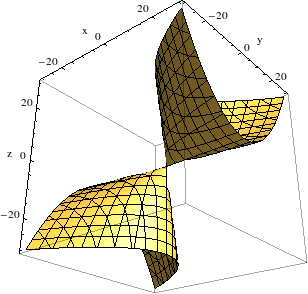
\includegraphics[scale=0.8,keepaspectratio=true]{./scone.png} \\
    The surface $y^2=xz$ in $\R^3.$
\end{figure}
 
\end{Example}

\begin{Example} Take $N=\Z^3$ and $\sigma = \Cone(e_1, e_2, e_3, e_1+e_3-e_2).$ Then $\sigma^{\V}$ consists of the points $(x,y,z)$ whose coordinates are all nonnegative and that satisfy $x+z\geq y.$ The semigroup $S_{\sigma}$ is generated by $e_1, e_3, e_1+e_2$ and $e_2+e_3$ and so we have $U_{\sigma} = \Spec K[X_1, X_3, X_1X_2, X_2X_3].$ Consider the $K$-algebra homomorphism $\varphi:K[W,X,Y,Z] \to K[X_1, X_3, X_1X_2, X_2X_3]$ which sends $W\mapsto X_1, X\mapsto X_2, Y\mapsto X_1X_2$ and $Z\mapsto X_2X_3$ and let $I:=\ker \varphi.$ We have $I\subseteq \ker \varphi.$ Now suppose $p(W,X,Y,Z)\in \ker \varphi.$ Since $WZ-XY \in I,$ so by replacing every instance of $XY$ by $WZ$ we can write $$p(W,X,Y,Z) = \sum a_{ijk} w^i x^j z^k + \sum b_{i'j'k'} w^{i'} y^{j'} z^{k'} + g(W,X,Y,Z)$$ where $g\in I.$ Since $p\in \ker I$ we have $$ \sum a_{ijk} X_1^i X_2^k X_3^{j+k} + \sum b_{i'j'k'} X_1^{i'+j'} X_2^{j'+k'} X_3^{k'} =0.$$

Therefore the coefficients $a_{ijk}, b_{i'j'k'}$ must be zero except possibly when a monomial of the same type appears in both sums. This condition on the exponents is $j=j'=0, i=i'$ and $k=k'.$ In that case, the equation displayed above implies $a_{ijk} = -b_{ijk}.$ Therefore the $a_{ijk}, b_{i'j'k'}$ coefficients are either zero or cancel each other, so $p(W,X,Y,Z) = g(W,X,Y,Z)\in I.$ Hence $I=\ker \varphi$ and $$ K[X_1, X_3, X_1X_2, X_2X_3]\cong K[W,X,Y,Z]/(WZ-XY).$$ So $U_{\sigma} = \Spec K[W,X,Y,Z]/(WZ-XY) = V(WZ-XY)\subset K^4.$ This variety is not smooth as it has a singularity at the origin.
\end{Example}

In the examples we have just seen, we realised affine toric varieties as varieties defined by {\em monomial equations}. In fact, this is a general feature whose proof is left as an exercise in \cite[Page.~ 19]{Fulton:Toric}. 

\begin{Theorem}\label{Monomial} Suppose $S_{\sigma}$ is generated by $\mu_1, \ldots, \mu_k.$ Then $U_{\sigma} = V(I_{\sigma}) \subseteq K^k,$ where $$ I_{\sigma} = \langle \  X_1^{a_1} X_2^{a_2} \cdots X_k^{a_k} - X_1^{b_1} X_2^{b_2} \cdots X_k^{b_k} \  \big| \  a_1 \mu_1 + \ldots +a_k \mu_k = b_1 \mu_1 + \ldots + b_k \mu_k \ \rangle.$$
\end{Theorem}

\begin{proof}
 By \ref{Iso} we have $K[S_{\sigma}] = K[\chi^{\mu_1}, \ldots, \chi^{\mu_k}].$ Then $K$-algebra homomorphism $$\varphi: K[X_1,\ldots, X_k] \to K[S_{\sigma}] \ : \ X_i\mapsto \chi^{\mu_i}$$ is surjective so $K[S_{\sigma}] \cong K[X_1,\ldots, X_k]/(\ker \varphi).$ We need to show that $I_{\sigma} = \ker \varphi.$ It is clear that $I_{\sigma}\subseteq \ker \varphi.$ For $\mu \in S_{\sigma}$ let $\pi(\mu) = \{ a=(a_1,\ldots, a_k) \ | \ a_1 \mu_1 + \ldots a_k \mu_k = \mu \}$ and adopt the notation $X^a := X_1^{a_1} \cdots X_k^{a_k}.$ Suppose $p= \sum \lambda_a X^a$ is in $\ker \varphi$ so $\displaystyle \varphi(p) = \sum_{\mu \in S_{\sigma}} \left( \sum_{a\in \pi(\mu) } \lambda_a \right) \chi^{\mu}=0.$ Therefore $\displaystyle \sum_{a\in \pi(\mu)} \lambda_a =0$ for all $\mu \in S_{\sigma}.$ We can write $\displaystyle p=\sum_{\mu \in S_{\sigma}} p_{\mu}$ where $\displaystyle p_{\mu} = \sum_{a\in\pi(\mu)} \lambda_a X^a$ so it suffices to show that $p_{\mu} \in I_{\sigma}.$ The number of non-zero coefficients of $p_{\mu}$ is finite, so suppose there are $m$ of them indexed with superscripts. We have 
 \begin{align*}
   \sum_{i=1}^m \lambda_{a^i} X^{a^i} &= \lambda_{a^1} ( X^{a^1} - X^{a^2} ) + (\lambda_{a^1} + \lambda_{a^2} ) (X^{a^2} -X^{a^3}) + \ldots\\
   &  +\left(\sum_{i=1}^{m-1} \lambda_{a^i}\right) ( X^{a^{m-1}} - X^{a^m} ) + \left(\sum_{i=1}^{m} \lambda_{a^i}\right)( X^{a^m} - X^{a^1}). \\
 \end{align*}
Since $\displaystyle \sum_{i=1}^{m} \lambda_{a^i}=0$ we see that $p_{\mu}$ is the sum of elements of $I_{\sigma},$ which completes the proof.
\end{proof}

It algebraic geometry it is often used that a ring homomorphism $\varphi: A \to B$ induces the following map of the prime spectrums: $\phi^*: \operatorname{PrimeSpec}(B) \to \operatorname{PrimeSpec}(A) \ , \ P \mapsto \varphi^{-1}(P).$ For our  approach (considering only maximal ideals) to work similarly we will need to ensure that if $A$ and $B$ are finitely generated $K$-algebras with no zero divisors and $\varphi:A\to B$ is a map of $K$-algebras, then we still have an induced map on their associated varieties: $\varphi^*: \Spec(B) \to \Spec(A) \ , \ M \mapsto \varphi^{-1}(M).$ The preimage of a maximal ideal is not always maximal, so we must show that this map is well defined. 

\begin{Lemma}\label{Max}
 Let $\varphi:A\to B$ be a map of finitely generated $K$-algebras. If $M$ is a maximal ideal of $B,$ then $\varphi^{-1}(M)$ is a maximal ideal of $A.$
\end{Lemma}

\begin{proof}
The ring $C:= B/M$ is a finitely generated $K$-algebra, so by Noether normalisation (see for example, \cite[Page.~ 63, \S 4.6]{Reid:Algebra}) it follows that there is a subset $\{ y_1, \ldots, y_r\}$ of $C$ where the $y_i$ are algebraically independent over $K$ and $C$ is integral over $K[y_1,\ldots, y_r].$ Since $M$ is a maximal ideal of $B,$ $C$ is a field. Recall that if $R\subseteq S$ is an integral extension of integral domains, then $R$ is a field if and only if $S$ is a field (see \cite[Page.~ 66, \S 4.9]{Reid:Algebra}). So $K[y_1,\ldots, y_r]$ is a field. Therefore we must have $r=0$ and $K[y_1,\ldots, y_r]=k.$ Therefore $C$ is integral, and hence algebraic, over $K.$ So $C$ is generated over $K$ by finitely many algebraic elements, and so it is a finite extension of $K.$ We have that $A/\varphi^{-1}(M)$ is isomorphic to some subalgebra of $C,$ so (abusing notation slightly) we have $K\subseteq A/\varphi^{-1}(M) \subseteq C.$ Since the extension $K\subseteq C$ is finite, so is the extension $K\subseteq A/\varphi^{-1}(M).$ Again using the fact that in an integral extension of domains $R\subseteq S,$ $R$ is a field if and only if $S$ is a field, we have $A/\varphi^{-1}(M)$ is a field. 
\end{proof}

A semigroup homomorphism $\varphi: S \to S'$ determines a map $K[S] \to K[S']$ by sending $\chi^{\mu}$ to $\chi^{\varphi (\mu)}.$ This induces a map $\Spec (K[S']) \to \Spec (K[S]).$ In particular, if $\tau \leq \sigma$ we have a morphism $U_{\tau} \to U_{\sigma}.$

\begin{Lemma}\label{faceopen} If $\tau$ is a face of $\sigma,$ there is a natural map $U_{\tau} \to U_{\sigma}$ which embeds $U_{\tau}$ as a principal open subset of $U_{\sigma}.$ 
\end{Lemma}

\begin{proof} Since $\tau$ is a face we can write $\tau = \sigma \cap u^{\perp}$ for some $u\in S_{\sigma}.$ By \ref{semigroup 1} we have $S_{\tau} = S_{\sigma} + \Z_{\geq 0} (-u).$ Hence for any $w'\in \tau$ we have $w' = w-pu$ for some $w\in S_{\sigma}, p\in \Z_{\geq 0}.$ In $K[S_{\tau}]$ this is $\chi^{w'} = \chi^w (\chi^{-u})^p,$ so $K[S_{\tau}] = K[S_{\sigma}][(\chi^u)^{-1}].$ The coordinate ring of $U_{\tau}$ is the localisation  of the coordinate ring of $U_{\sigma}$ at $\chi^u$ so the corresponding map $U_{\tau} \to U_{\sigma}$ embeds $U_{\tau}$ as a principal open subset of $U_{\sigma}.$
Since $\tau\leq \sigma$ we have $\sigma^{\V} \cap M \subseteq \tau^{\V} \cap M.$ The inclusion $S_{\sigma} \to S_{\tau}$ determines the $K$-algebra inclusion $K[S_{\sigma}] \to K[S_{\tau}]=K[S_{\sigma}][(\chi^u)^{-1}].$ This map is the natural map associated to the localisation of $K[S_{\tau}]$ at $\chi^u.$ Recall that the natural map associating to localisation a coordinate ring $K[V]$ at $f$ induces an embedding of the principal open subset $V_f$ into $V.$ 
\end{proof} 

\begin{Theorem}\label{torusdenseaffine}
Affine toric varieties contain an algebraic torus as an open dense subset.
\end{Theorem}
\begin{proof} The reason we demand that our cones are strongly convex is to ensure (by \ref{strongzero}) the zero cone $\{ 0\}$ is a face of every cone. Lemmas \ref{faceopen} and \ref{zerotorus} then imply that an algebraic torus is embedded as an open subset of all affine toric varieties. Further, the map $(K^*)^n \to U_{\sigma}$ is induced by an injective map on coordinate rings $K[S_{\sigma}] \to K[S_{0}]$ so it has dense image.
\end{proof}

\begin{Remark} 
We have purposely avoided using the fact that open subsets of irreducible spaces are dense in the previous proof. Our approach provides another perspective to the irreducibility of affine toric varieties. An algebraic torus is irreducible and since topological spaces that have irreducible dense subspaces are irreducible we see again that affine toric varieties are deserving of their name. We can view the same argument algebraically as follows: Our construction of affine toric varieties was such that their coordinate rings are (by \ref{Iso}) isomorphic to subrings of the integral domain $K[X_1, X_1^{-1}, \ldots, X_n, X_n^{-1}].$ Therefore these coordinate rings are integral domains themselves, implying the irreducibility of their corresponding variety.
\end{Remark}
The bijective correspondence between points of an affine variety and the maximal ideals of its coordinate ring is useful because it allows geometric problems to be attacked with algebraic techniques. In the case of affine toric varieties, we have yet another useful way to view points. 

\begin{Theorem} \label{SemigroupPoints}
Let $U_{\sigma}$ be an affine toric variety. There are natural bijections between any pair of the sets below:
 
 \begin{itemize}
  \item Points of $U_{\sigma}$
  \item Maximal ideals of $K[S_{\sigma}]$
  \item $K$-algebra homomorphisms $K[S_{\sigma}]\to K$
  \item Semigroup homomorphisms $S_{\sigma} \to (K, \times)$
 \end{itemize}

\end{Theorem}

\begin{proof}
 The bijections amongst the first three are standard and can be found in most elementary texts on algebraic geometry (for example, \cite{Shafarevich1}). We exhibit the bijection between the last two. Let $\varphi: K[S_{\sigma}] \to K$ be a $K$-algebra homomorphism. Then we have a corresponding semigroup homomorphism $\tilde{\varphi}: S_{\sigma} \to K$ by $\tilde{\varphi}(u) = \varphi( \chi^u ).$ Given a semigroup homomorphism $\phi: S_{\sigma} \to K$ we define a $K$-algebra homomorphism $\phi': K[S_{\sigma}]\to K$ to be the unique linear map such that $\phi'(\chi^u) = \phi(u).$ These two correspondences are mutually inverse to each other and therefore bijections.  
\end{proof}

\begin{Lemma} \label{coneproduct} Let $\sigma$ be a cone in a lattice $N$ and $\sigma'$ a cone in a lattice $N'.$ Then $\sigma \times \sigma'$ is a cone in $N\oplus N'$ and $U_{\sigma \times \sigma'} = U_{\sigma} \times U_{\sigma'}.$
\end{Lemma}

\begin{proof} It suffices to show the corresponding identity on coordinate rings: $K[S_{\sigma \times \sigma'} ] \cong K[S_{\sigma}] \otimes K[S_{\sigma'}].$ We are ensured by Gordan's lemma (\ref{Gordan}) that $S_{\sigma}$ has finitely many generators $a_1, \ldots, a_n$ and $S_{\sigma'}$ has finitely many generators $b_1, \ldots, b_m.$ Then $S_{\sigma \times \sigma'}$ is generated by $(a_1,0),\ldots, (a_n,0),$ $ (0,b_1), \ldots, (0,b_m).$ The coordinate rings are $K[S_{\sigma}] = K[\chi^{a_1}, \ldots, \chi^{a_n}] , K[S_{\sigma'}] = K[\eta^{b_1}, \ldots, \eta^{b_m} ] $ and $K[S_{\sigma \times \sigma'}] = K[\chi^{a_1}, \ldots, \chi^{a_n}, \eta^{b_1}, \ldots, \eta^{b_m} ].$ Let $\varphi: K[S_{\sigma}] \otimes K[S_{\sigma'}]$ be the $K$-algebra homomorphism defined by $x \otimes y \mapsto xy.$ The $K$-algebra map $\phi: K[S_{\sigma\times \sigma'}] \to K[S_{\sigma}] \otimes K[S_{\sigma'}]$ which sends $\chi^a \eta^b \mapsto \chi^a \otimes \eta^b$ is well defined because there are no relations between the $\chi$ and $\eta$ terms. It is mutally inverse to $\varphi,$ so the required isomorphism holds.
\end{proof}

\begin{Lemma} \label{AffineToricMorphism} Let $\sigma, \sigma'$ be cones in $N$ and $N'$ respectively. Suppose $\Theta : N \to N'$ is a lattice homomorphism (a homomorphism of finite rank $\Z$-modules) such that $\Theta(\sigma)\subseteq \sigma'.$ Then $\Theta$ induces a morphism $U_{\sigma}\to U_{\sigma'}.$ If $\Theta$ is an isomorphism, then $U_{\sigma} = U_{\sigma'}.$
\end{Lemma}
 
\begin{proof} Let $M, M'$ denote the dual spaces of $N$ and $N'$ respectively. The dual map of $\Theta$ is $\tilde{\Theta}:M'\to M$ which takes the function $s(-)\in M'$ and maps it to the function $s(\Theta(-))$ in $M.$ That is, $\tilde{\Theta}(s)(t) = s(\Theta(t)).$ If $s\in (\sigma')^{\V}$ then $\tilde{\Theta}(s)\in \sigma^{\V}$ because if $t\in \sigma$ then $\tilde{\Theta}(s)(t) = s(\Theta(t)) \geq 0.$ So $\tilde{\Theta}$ restricts to a map $\tilde{\Theta}:S_{\sigma'}\to S_{\sigma}.$ There are now several ways to realise the (same) morphism $U_{\sigma}\to U_{\sigma'}$ that $\tilde{\Theta}$ induces. Viewing points as semigroup homomorphisms into $K$ (see \ref{SemigroupPoints}), the induced map is $$ U_{\sigma} \to U_{\sigma'}\ : \ ( x: S_{\sigma} \rightarrow K ) \mapsto ( x\circ \tilde{\Theta}: S_{\sigma'} \rightarrow K ).$$ Viewing points as maximal ideals, the morphism $U_{\sigma}\to U_{\sigma'}$ is the one induced from the $K$-algebra homomorphism $$ K[S_{\sigma'}] \to K[S_{\sigma}]\ : \  \chi^u \mapsto \chi^{\tilde{\Theta}(u)}.$$ If $\Theta$ is an isomorphism then so is this $K$-algebra map, in which case $U_{\sigma} = U_{\sigma'}.$
\end{proof}


\section{Algebraic Varieties}
For the reader who has only studied varieties in a classical setting, this section is intended to introduce {\em algebraic varieties}, the class of objects into which toric varieties will fall. Indeed, toric varieties are some of the most simple examples algebraic varieties and learning about their construction will aid in ones understanding about what an algebraic variety is. Our definition of algebraic variety is that of Kempf's \cite{Kempf} with only minor differences in terminology, and there the reader will find plenty of introductory and accessible material, including proofs of any claims made in this section. Kempf sacrifices generality in the interest of reaching algebraic varieties as soon as possible. One can also refer to Mumford's Red Book (\cite{MumfordRedBook}), which is written at a slightly more advanced level and takes some extra time to study ringed spaces more generally. Mumford takes essentially the same definition also requires algebraic varieties to be irreducible and separated, a notion we will discuss at the end of this section.
~
\begin{Definition}
Let $F$ be a fixed field and $X$ be a topological space. A {\em sheaf of regular functions} $\mathcal{O}_X$ on $X$ assigns to each open subset $U\subseteq X$ an $F$-algebra $\mathcal{O}_X(U)$ of functions $U\to F$, which we say consists of all {\em regular functions on} $U,$ satisfying two conditions:
  \begin{itemize}
   \item If $U=\cup U_{i}$ is a union of open subsets and $f:U\to F$ is an $F$ valued function on $U,$ then $f$ is regular on $U$ if and only if the restriction $f|_{U_{\alpha}}$ is regular on each $U_{\alpha}.$
   \item If $f$ is a regular function on an open subset $U$ then $D(f):= \{ u\in U \ | \ f(u)\neq 0 \}$ is open and $1/f$ is regular on $D(f).$
  \end{itemize}
If $\mathcal{O}_X$ is a sheaf of regular functions on $X$ then we call the pair $(X,\mathcal{O}_X)$ a {\em ringed space}. Often it is clear what the sheaf associated to a ringed space is and in that case we simply write $X$ to denote the ringed space.
\end{Definition}
~
We note that the definitions we have given for ringed spaces and sheaves is actually only a special case of the general definition that one finds in the literature, but they are sufficient for our purposes in defining algebraic varieties. 
\begin{Example}
~
\begin{itemize}
 \item Take $F=\R$ or $\C,$ and any topological space $X.$ There is a natural sheaf where we take $\mathcal{O}_X(U)$ to be the set of all continuous functions $U\to F.$ 
 \item An open subspace $Y$ of a ringed space $X$ is naturally a ringed space itself. For any open subset $U\subseteq Y$ take $\mathcal{O}_Y(U) = \mathcal{O}_X(U).$
\end{itemize}
\end{Example}

\begin{Definition}
 A {\em morphism} $f:X\to Y$ of ringed spaces is a continuous map which {\em pulls-back} regular functions into regular functions. That is to say, if $g(-)$ is a regular function on an open subset $V\subseteq Y$ then $f^*(g)(-):= g(f(-))$ is a regular function on the open subset $f^{-1}(V)$ of $X.$ Pulling-back by $f$ induces an $F$-algebra homomorphism $$ f^*: \mathcal{O}_Y(V) \to \mathcal{O}_X( f^{-1}(V) )$$ for each open subset $V$ of $Y.$ We say $f$ is an {\em isomorphism} if it is bijective and $f^{-1}$ is a morphism as well. 
\end{Definition}

\begin{Example}
 The identity $\operatorname{id}_X$ on a ringed space $X$ is a morphism, as is the composition of morphisms. The inclusion $U\to X$ of an open subspace into a ringed space is a morphism. If $X$ and $Y$ are topological spaces with sheafs of continuous functions as defined in the previous example, then any continuous map $X\to Y$ is a morphism. 
\end{Example}

\begin{Definition} 
 Let $K$ be an algebraically closed field and $X,Y$ be ringed spaces. Let the map $$ *: \operatorname{Morphism}(X,Y) \to \Hom_{K-\text{alg}} ( \mathcal{O}_Y, \mathcal{O}_X )$$ send a morphism $f:X\to Y$ to its induced $F$-algebra map $ f^*: \mathcal{O}_Y(V) \to \mathcal{O}_X( f^{-1}(V) ).$ An {\em affine variety} $Y$ is a ringed space such that $*$ is bijective for every $X$ and $\mathcal{O}_Y$ is finitely generated as a $K$-algebra. An {\em (algebraic) variety} $X$ is a ringed space which is of {\em finite type} i.e. it has a finite open covering by affine varieties. We say $K[X]:= \mathcal{O}_X(X)$ is the {\em coordinate ring} of a variety. 
\end{Definition}

We do not demand that varieties are irreducible or separated (we will discuss this below).
\begin{Example}
 Suppose $V\subseteq K^n$ is an irreducible algebraic set and $K[V]$ its usual coordinate ring with field of fractions $K(V).$ Recall that we can view elements of $K[V]$ as polynomial functions $V\to K.$ For $x\in V,$ let $\mathfrak{m}_x$ denote the maximal ideal which is the kernel of the map $K[V] \to K$ which evaluates polynomials at $x.$ Let $\mathcal{O}_x := K[V]_{ \mathfrak{m}_x} = \{ f/g \ | \ f,g\in K[V] \ , \ g(x)\neq 0 \}.$ For open subsets $U$ of $V,$ let $\mathcal{O}_V(U) = \cap_{x\in U} \mathcal{O}_x.$ All of the $\mathcal{O}_V(U)$ are subrings of $K(V),$ and we can view their elements as functions $U\to K.$ This defines a sheaf of regular functions of $V$ which allows us to view irreducible algebraic sets as affine varieties.
\end{Example}

The new definitions of affine variety, morphism and coordinate ring include the classical ones. All affine and projective algebraic sets are algebraic varieties. Every affine variety is isomorphic as a ringed space to an irreducible algebraic subset of affine space. Thus an algebraic variety is a topological space which locally looks like an affine variety. One may find it useful to draw analogy with the definition of a manifold. 

The following proposition controls the varieties we can attain from glueing.
\begin{Proposition}
 Let $V=\cup_{i=1}^n V_i$ be a covering of a topological space $V$ by finitely many algebraic varieties. Suppose the following {\em glueing condition} holds: For all $i,j,$ $V_i\cap V_j$ is open in both $V_i$ and $V_j$ and $\mathcal{O}_{V_i}|_{V_i\cap V_j}=\mathcal{O}_{V_j}|_{V_i\cap V_j}.$ Then there is a unique sheaf on $V$ which satisfies the following:
   \begin{enumerate}
    \item $V$ is an algebraic variety.
    \item Each inclusion $V_i\to V$ is an isomorphism of $V_i$ onto an open set.
    \item For each $i=1,\ldots, n,$ $\mathcal{O}_V|_{V_i} = \mathcal{O}_{V_i}.$
   \end{enumerate}
To give a regular map from $V$ to a variety $W$ amounts to giving a family of regular maps $\varphi:V_i\to W$ such that $\varphi_i|_{V_i\cap V_j}=\varphi_j|_{V_i\cap V_j}.$
\end{Proposition}

\begin{proof}(\cite[Chapter 4, Prop.~ 4.13]{Milne}) The collection of subsets $U\subseteq V$ such that $U\cap V_i$ is open for all $i$ is the unique topology on $V$ satisfying condition b) above. The assignment $\mathcal{O}_V(U) = \{ f:U\to K \ | \ f|_{U\cap V_i} \in \mathcal{O}_{V_i}(U\cap V_i) \forall \ i=1,\ldots n \}$ is the only sheaf of $K$-algebras satisfying condition c). With these specifications, $V$ is an algebraic variety. To prove the last statement note that since each $(V_i, \mathcal{O}_{V_i})$ is a union of finitely many affine varieties, so is $(V,\mathcal{O}_V).$ Moreover, giving a map $\varphi:V\to W$ amounts to giving a family of maps $\varphi_i:V_i\to W$ such that $\varphi_i|_{V_i\cap V_j}=\varphi_j|_{V_i\cap V_j}.$ By definition, $\varphi$ is regular if and only if $\varphi|_{V_i}$ is regular for each $i.$ 
\end{proof}

Suppose we have two algebraic subsets $V(I)\subseteq \mathbb{A}^n, V(J) \subseteq \mathbb{A}^m$ where $I\subseteq K[X_1,\ldots, X_n]$ and $J\subseteq K[Y_1,\ldots, Y_m]$ respectively. Recall that their product variety is given by $V(I \sqcup J) \subseteq \mathbb{A}^{n+m},$ and that the topology on $\mathbb{A}^{n+m}$ is not simply the product topology of the affine spaces $\mathbb{A}^n, \mathbb{A}^m.$ We wish to define the product of two varieties. 
\begin{Definition}
 We define the {\em product} of two varieties $V$ and $W.$ Write $V=\cup V_i, W=\cup W_j$ as finite unions of open subsets which are affine varieties. Note that $V$ can be viewed as the variety obtained by the glueing of $(V_i, \mathcal{O}_{V_i})$ as in the previous proposition, and similarly for $W.$ Then $$ V \times W = \cup ( V_i \times W_j)$$ and the $(V_i \times W_j, \mathcal{O}_{V_i\times W_j})$ satisfy the glueing condition. Therefore we can define $(V\times W, \mathcal{O}_{V\times W})$ to be the variety obtained by glueing the $(V_i \times W_j, \mathcal{O}_{V_i\times W_j}).$ 
\end{Definition}
Milne proves in \cite[Chapter 4, Prop.~ 4.21]{Milne} that the sheaf obtained from the above construction is independent of the coverings. 

We create manifolds by glueing together pieces of Euclidean space, but when we do this it is very easy to induce strange properties. As we are identifying points we can expect to lose things like the uniqueness of limits. To keep the study more relevant to our idea of geometry, we impose an extra condition that our resulting space is Hausdorff. Perhaps its most used consequence is that continuous functions on the space which agree on a dense subset agree everywhere, or equivalently, that the set where two continuous functions agree should be closed. Our definition of a variety has been general enough to allow pathologies contradicting such intuitions. 

\begin{Example}
 Let $A_1, A_2$ be two copies of $\mathbb{A}^1(K)$ and form the topological disjoint union $V^*= A_1 \sqcup A_2.$ Define an equivalence relation by $ x \in V_1 \sim y \in V_2$ if and only if $x=y$ and $x\neq 0,$ and form the quotient topological space $V=V^*/\sim.$ That is, we are glueing two copies of the affine line by identifying equal non-zero points in each copies. We have $V = A_1 \cup A_2$ and $A_1 \cap A_2 = \mathbb{A}^1\setminus\{0\}.$ A function on an open subset is regular if its restriction to each $A_i$ is regular. Thus $V$ is a variety, often called the {\em line with two origins}. Let $f,g$ denote the isomorphisms of $\mathbb{A}^1$ with $A_1, A_2$ respectively. These give regular functions $f,g: \mathbb{A}^1 \to X$ that agree on the non-closed set $\mathbb{A}^1\setminus \{ 0 \}.$ The rings of regular functions at the origins coincide: $\mathcal{O}_{0} = \mathcal{O}_{0'}.$ Two distinct points have the same ring of regular functions, and any functions in this ring takes the same value at $0$ and $0'.$ In this sense the points $0$ and $0'$ can not be separated by regular functions.
\end{Example}

We would like a condition that prevents such pathologies occurring in algebraic varieties, but the Zariski topology is almost never Hausdorff so we need to find a substitute. The key lies in the characterisation of a topological space $X$ as Hausdorff if and only if the image of the diagonal map $D:X\to X\times X \ : \ x\mapsto (x,x)$ is a closed subset of the product space $X\times X$ (with the product topology). We alter this condition slightly.

\begin{Definition}
 Let $V$ be a variety. We say that $X$ is {\em separated} if it satisfies the {\em Hausdorff axiom}, which demands that the image of the diagonal morphism $D:X\to X \times X \ : \ x\mapsto (x,x)$ is closed in the product of varieties $X\times X.$ 
\end{Definition}
Note that all affine algebraic sets $V(I)\subseteq \mathbb{A}^n$ are separated, as it is not hard to write down the ideal $J\in K[X_1,\ldots, X_n, Y_1,\ldots, Y_n]$ for which $V(J) = V(I) \times V(I) \subseteq \mathbb{A}^{2n}.$ 

\begin{Proposition}
 A variety $X$ is separated if and only if for all varieties $Y$ and for all morphisms $f,g:Y\to X,$ we have that $\{ y\in Y \ | \ f(y)=g(y) \}$ is a closed subset of $Y.$
\end{Proposition}
\begin{proof}
 Morphisms $f,g:Y\to X$ induce a morphism $(f,g):Y \to X \times X \ : \ y \mapsto ( f(y), g(y) ).$ Since $\{ y\in Y \ | \ f(y)=g(y) \} = (f,g)^{-1} ( D(X)),$ it is closed if $D(X)$ is closed i.e. if $X$ is separated. Conversely, let $Y=X\times X$ and $f,g:X\times X \to X$ be projections into the first and second coordinates respectively. Then $D(X) = \{ x\in X\times X \ | \ f(x)=g(x) \},$ and this being closed means $X$ is separated. 
\end{proof}



\section{Abstract Toric Varieties}

We have seen how to create an affine variety from a cone. By identifying along certain open subsets we can glue together affine varieties to produce an algebraic variety. The interested reader can consult Eisenbud and Harris' \cite[Page.~ 33, \S I.2.4.]{EisenbudHarris} for more details about glueing varieties, however it is not required here. We construct general toric varieties through a particularly simple example of the glueing construction. 

\begin{Definition}
 A {\em fan} $\Delta$ in a lattice $N$ is a finite set of cones such that each face of a cone in $\Delta$ is also a cone in $\Delta$ and the intersection of two cones in $\Delta$ is a face of each cone. The {\em abstract toric variety} $X(\Delta)$ constructed from a fan is the topological disjoint union of all the affine toric varieties $U_{\sigma}$ associated to a cone $\sigma\in \Delta$ glued together by the following rule. If $\sigma$ and $\sigma'$ are cones in $\Delta$ then $\sigma\cap \sigma'$ is a face of both, so by \ref{faceopen} we have natural maps $$ \imath: U_{\sigma\cap \sigma'} \to U_{\sigma} \ , \ \imath': U_{\sigma\cap \sigma'} \to U_{\sigma'}.$$ We glue $U_{\sigma}$ and $U_{\sigma'}$ by identifying the images of each point in $U_{\sigma \cap \sigma'}$ under these maps, for every point in $U_{\sigma \cap \sigma'}.$ Doing this for every pair of cones in $\Delta$ produces $X(\Delta).$
\end{Definition}

By definition $X(\Delta)$ has a finite open covering by the open sets $\{ U_{\sigma} \ | \ \sigma \in \Delta \},$ $X(\Delta)$ is an algebraic variety. We do some detailed computations of some examples to get a better understanding of these objects before we prove results about them.  

\begin{Example}[One dimensional toric varieties]\label{OneDim}
Let $N=\Z$ and $\Delta = \{0, \sigma, \sigma'\}$ as shown below:
\begin{figure}[ht]
  \centering
  \begin{tikzpicture}
    \draw [thin, gray,-latex] (0,0) -- (4,0);% Draw x axis
  \draw [thin, gray,-latex] (0,0) -- (-4,0);% Draw x axis
\foreach \x in {-4,-2,0,2,4}{% Two indices running over each
      \foreach \y in {0}{% node on the grid we have drawn 
        \node[draw,circle,inner sep=1pt,fill] at (\x,\y) {};}}
\draw [ultra thick,-latex,blue] (0,0)
        -- (2,0) node [below ]{$e_1$};
\draw [ultra thick,-latex,blue] (0,0)
        -- (-2,0) node [below] {$-e_1$};
\draw [blue] (0,0) node [below]{0};
\draw (-0.7,0.5) node{\scalebox{1.2}{$\sigma'$ }};
\draw (0.9,0.45) node{\scalebox{1.2}{$\sigma$ }};
  \end{tikzpicture}
\end{figure}

We have $\sigma = \sigma^{\V} = \Cone(e_1)$ so $S_{\sigma}$ is generated by $e_1$ so $K[S_{\sigma}] = K[X].$ Similarly, $\sigma' = (\sigma')^{\V} =\Cone(-e_1)$ so $S_{\sigma'}$ is generated by $-e_1$ so $K[S_{\sigma'}]=K[X^{-1}].$ As usual, $K[S_{0}] = K[X,X^{-1}].$ Both $U_{\sigma}$ and $U_{\sigma'}$ are copies of $K$ and $X(\Delta)$ is obtained by gluing the images of the embeddings $$ \imath : U_0 = \Spec K[X,X^{-1}] \to U_{\sigma} = \Spec K[X] $$ $$ \ \imath': U_{0} = \Spec K[X,X^{-1}] \to U_{\sigma'} = \Spec K[X^{-1}] . $$ Let $\m_a$ be the maximal ideal of $K[X,X^{-1}]$ corresponding to $a\in K^*.$ It is the kernel of the evaluation map $\epsilon_a: K[X,X^{-1}] \to K$ that sends $p(X,X^{-1}) \mapsto p(a,a^{-1}).$ We compute $\imath(\m_a) = \m_a \cap K[X] = \{ \text{polynomials in} \ K[X] \text{ such that} \ p(a)=0 \} = (X-a)$ which is the ideal corresponding to the point $X=a.$ Similarly, $\imath'(\m_a) = \m_a \cap K[X^{-1}] = \{ \text{polynomials in} \ K[Y] \text{ such that} \ p(a^{-1})=0 \}$ which is the ideal corresponding to the point $X=a^{-1}.$ Therefore we have $$X(\Delta) = \frac{ K \bigsqcup K}{ (a \sim a^{-1})_{a\neq 0} }.$$ Recall the construction of the complex projective line $\Proj^1(K).$ It is covered by two copies of the affine line: $\Proj^1(K) = \{ [x:1] \ | \ x\in K \} \cup \{ [1:x] \ | \ x\in K \}$ where the overlap is glued via the identification $[a:1] = [1:a^{-1}]$ for all $a\neq 0.$ This is the exact same construction as the toric variety, so $X(\Delta) = \Proj^1(K).$ The only other one dimensional fans are $\{\sigma, 0 \} , \{ \sigma', 0 \}$ and $\{ 0\}$ which correspond to $K, K $ and $K^*$ respectively. So the only one dimensional toric varieties are $K^*, K$ and $\Proj^1(K).$
\end{Example}

\begin{Example}[Complex projective space as a toric variety] \label{ProjFan}
Let $N=\Z^2$ and $\Delta$ be the fan consisting of the following three cones and all of their faces.

    \begin{figure}[ht]
  \centering
  \begin{tikzpicture}
    \draw [thin, gray,-latex] (-3,0) -- (3,0);% Draw x axis
    \draw [thin, gray,-latex] (0,-3) -- (0,3);% Draw y axis
    \clip (-3.05,-3.05) rectangle (3.05cm,3.05cm); 
    \draw[style=help lines,dashed] (-4,-4) grid[step=1cm] (4,4);
    \foreach \x in {-5,-4,...,5}{% Two indices running over each
      \foreach \y in {-5,-4,...,5}{% node on the grid we have drawn 
        \node[draw,circle,inner sep=1pt,fill] at (\x,\y) {};}}
    \draw [ultra thick,-latex,blue] (0,0)
        -- (0,1) node [below left] {$e_2$};
    \draw [ultra thick,-latex,blue] (0,0)
        -- (1,0) node [below left] {$e_1$};
\draw [ultra thick,-latex,blue] (0,0)
        -- (-1,-1) node [above left] {$-e_1-e_2$};
    \filldraw[fill=gray, fill opacity=0.25, draw=black] (0,0) -- (0,3) -- (3,3) -- (3, 0) -- (0,0);
    \filldraw[fill=gray, fill opacity=0.45, draw=black] (0,0) -- (3,0) -- (3,-3) -- (-3, -3) -- (0,0);
    \filldraw[fill=gray, fill opacity=0.35, draw=black] (0,0) -- (0,3) -- (-3,3) -- (-3, -3) -- (0,0);
    \draw (1.5,1.5) node{\scalebox{1.5}{$\sigma_1$ }};
\draw (-1.4,0.5) node{\scalebox{1.5}{$\sigma_2$ }};
\draw (0.6,-1.5) node{\scalebox{1.5}{$\sigma_3$ }};
  \end{tikzpicture}
  \label{figure:lattice9}
\end{figure}

The cone $\sigma_1^{\V}$ consists of the $(x,y)$ such that $x\geq 0$ and  $y\geq 0.$ The cone $\sigma_2^{\V}$ consists of the $(x,y)$ such that $y\geq 0$ and $-x-y\geq 0.$ The cone $\sigma_3^{\V}$ consists of the $(x,y)$ such that $-x-y\geq 0$ and $x\geq 0.$ 
    \begin{figure}[ht]
  \centering
  \begin{tikzpicture}
    \draw [thin, gray,-latex] (-3,0) -- (3,0);% Draw x axis
    \draw [thin, gray,-latex] (0,-3) -- (0,3);% Draw y axis
    \clip (-3.05,-3.05) rectangle (3.05cm,3.05cm); 
    \draw[style=help lines,dashed] (-4,-4) grid[step=1cm] (4,4);
    \foreach \x in {-5,-4,...,5}{% Two indices running over each
      \foreach \y in {-5,-4,...,5}{% node on the grid we have drawn 
        \node[draw,circle,inner sep=1pt,fill] at (\x,\y) {};}}
    \draw [ultra thick,-latex,blue] (0,0)
        -- (0,1) node [below right] {$e_2$};
    \draw [ultra thick,-latex,blue] (0,0)
        -- (1,0) node [above left] {$e_1$};
    \draw [ultra thick, -latex,blue] (0,0)
	-- (1,-1);
    \draw [ultra thick, -latex,blue] (0,0)
	-- (0,-1);
    \draw [ultra thick, -latex,blue] (0,0)
	-- (-1,0);
\draw [ultra thick,-latex,blue] (0,0)
        -- (-1,1) node [above left] {$-e_1+e_2$};
    \filldraw[fill=gray, fill opacity=0.25, draw=black] (0,0) -- (0,3) -- (3,3) -- (3, 0) -- (0,0);
    \filldraw[fill=gray, fill opacity=0.45, draw=black] (0,0) -- (0, -3) -- (3,-3) -- (0,0);
    \filldraw[fill=gray, fill opacity=0.35, draw=black] (0,0) -- (-3,0) -- (-3,3) -- (0,0);
    \draw (1.5,1.5) node{\scalebox{1.5}{$\sigma_1^{\V}$ }};
\draw (-1.4,0.5) node{\scalebox{1.5}{$\sigma_2^{\V}$ }};
\draw (0.6,-1.5) node{\scalebox{1.5}{$\sigma_3^{\V}$ }};
  \end{tikzpicture}
  \label{figure:lattice7}
\end{figure}

Reading off the picture, $S_{\sigma_1}$ has generators $e_1, e_2$ we have $K[S_{\sigma_1}] = K[X,Y].$ The semigroup $S_{\sigma_2}$ has generators $-e_1, -e_1+e_2$ so $K[S_{\sigma_2}] = K[X^{-1} , X^{-1}Y].$ Similarly, $S_{\sigma_3}$ has generators $-e_2, e_1-e_2$ so $K[S_{\sigma_3}] = K[Y^{-1} , XY^{-1}].$ So we have three copies of $K^2$ with each pair overlapping on $U_{0} = (K^*)^2.$ The gluing construction does the following on the overlaps: We glue $(x,y)$ from $U_{\sigma_1}$ to $(x^{-1}, x^{-1}y)$ on $U_{\sigma_2}$ and to $(x^{-1}y, x^{-1})$ on $U_{\sigma_3}.$ We also glue $(x,y)$ from $U_{\sigma_2}$ to $(xy^{-1}, y^{-1})$ on $U_{\sigma_3}.$ Notice that $\Proj^2(K) = \{ [1:x:y] \ | \ (x,y) \in K^2 \}\cup \{ [x:1:y] \ | \ (x,y) \in K^2 \}\cup \{ [x:y:1] \ | \ (x,y) \in K^2 \}$ is three copies of $K^2$ glued via exactly the same rules. Therefore $X(\Delta) = \Proj^2(K).$ The same type of calculation works for arbitrary dimension. Suppose $N=\Z^d$ and let $e_0 = -(e_1+e_2+\ldots+e_d).$ Then $\Delta = \{ \Cone(E) \ | \ E\subset \{e_0, \ldots, e_d\} \}$ is a fan such that $X(\Delta) = \Proj^d(K).$
\end{Example}

\begin{Example}[The blow up of $K^2$ along the coordinate axes]
Take $N=\Z^2$ and let $\Delta =\{ 0, \sigma_1, \sigma_2\}.$

     \begin{figure}[ht]
  \centering
  \begin{tikzpicture}
    \draw [thin, gray,-latex] (-3,0) -- (3,0);% Draw x axis
    \draw [thin, gray,-latex] (0,-3) -- (0,3);% Draw y axis
    \clip (-3.05,-3.05) rectangle (3.05cm,3.05cm); 
    \draw[style=help lines,dashed] (-4,-4) grid[step=1cm] (4,4);
    \foreach \x in {-5,-4,...,5}{% Two indices running over each
      \foreach \y in {-5,-4,...,5}{% node on the grid we have drawn 
        \node[draw,circle,inner sep=1pt,fill] at (\x,\y) {};}}
    \draw [ultra thick,-latex,blue] (0,0)
        -- (0,1) node [below left] {$e_2$};
    \draw [ultra thick,-latex,blue] (0,0)
        -- (1,0) node [below left] {$e_1$};
  \draw [ultra thick,-latex,blue] (0,0)
        -- (0,-1) ;
    \draw [ultra thick,-latex,blue] (0,0)
        -- (-1,0) ;
    \filldraw[fill=gray, fill opacity=0.25, draw=black] (0,0) -- (0,3) -- (3,3) -- (3, 0) -- (0,0);
    \filldraw[fill=gray, fill opacity=0.25, draw=black] (0,0) -- (-3,0) -- (-3,-3) -- (0, -3) -- (0,0);
    \draw (1.6,1.5) node{\scalebox{1.5}{$\sigma_1$ }};
\draw (-1.4,-1.5) node{\scalebox{1.5}{$\sigma_2$ }};
  \end{tikzpicture}
  \label{figure:lattice8}
\end{figure}

Then $\sigma^{\V}_1=\Cone(e_1, e_2)$ and $\sigma_2^{\V} = \Cone(-e_1, -e_2).$ Thus $S_{\sigma_1}$ is generated by $e_1, e_2$ while $S_{\sigma_2}$ is generated by $-e_1, -e_2$ and therefore $K[S_{\sigma_1}] = K[X,Y], K[S_{\sigma_2}]=K[X^{-1}, Y^{-1}].$ The gluing construction identifies the images of the natural embeddings $$ \imath : U_0 = \Spec K[X,X^{-1},Y , Y^{-1}] \to U_{\sigma_1} = \Spec K[X,Y] $$ $$ \ \imath': U_{0} = \Spec K[X,X^{-1}, Y ,Y^{-1}] \to U_{\sigma_2} = \Spec K[X^{-1}, Y^{-1}] . $$
Let $(a,b)\in (K^*)^2$ and $\m_{a,b}$ be the maximal ideal of $K[X,X^{-1}, Y, Y^{-1}]$ corresponding to it. It is the kernel of the evaluation map $\epsilon_{a,b} : K[X,X^{-1},Y, Y^{-1}] \to K$ that sends $p(X,X^{-1}, Y, Y^{-1}) \mapsto p(a,a^{-1}, b, b^{-1}).$ We have $\imath(\m_{a,b}) = \m_{a,b} \cap K[X,Y]$ which corresponds to the point $(a,b),$ and $\imath'(\m_{a,b}) = \m_{a,b} \cap K[X^{-1}, Y^{-1}]$ which corresponds to the point $(a^{-1}, b^{-1}).$ Therefore $$ X(\Delta) = \frac{ K^2 \bigsqcup K^2 }{ \left( (a,b) \sim (a^{-1}, b^{-1}) \right)_{a,b\neq 0} }.$$ This object is more exotic than the previous examples. Readers familiar with blow ups may recognise this as the blow up of $K^2$ along the coordinate axes. Standard references to learn about blow ups are \cite[p.~ 602-610]{GriffithsHarris}, \cite[Chapter 4, \S 2]{EisenbudHarris}, \cite[Chapter 2, \S 4]{Shafarevich1} and \cite[Chapter 1]{Hartshorne}. A beautifully motivated and illustrated source is \cite{Brodmann}.
\end{Example}

\begin{Theorem} Toric varieties contain an algebraic torus as an open dense subset.
\end{Theorem}
\begin{proof} By \ref{torusdenseaffine}, $U_{\sigma}$ contains the algebraic torus as an open dense subset for every $\sigma \in \Delta.$ This torus is identified under the glueing construction, so it remains an an open dense subset of $X(\Delta).$
\end{proof}
\begin{Corollary}
 If $\Delta$ is a fan in an $n$ dimensional lattice then $X(\Delta)$ is an $n$ dimensional variety.
\end{Corollary}
\begin{proof}
 By \ref{zerotorus} and the previous theorem, $(K^*)^n$ is dense in $X(\Delta).$ Since $(K^*)^n$ is $n$ dimensional, so is $X(\Delta).$
\end{proof}


\begin{Proposition} If $\Delta$ is a fan in $N$ and $\Delta'$ is a fan in $N'$ then $\Delta \times \Delta' := \{ \sigma \times \sigma ' | \sigma \in \Delta, \sigma' \in \Delta' \}$ is a fan in $N \oplus N'$ and $X(\Delta \times \Delta') = X(\Delta) \times X(\Delta').$
\end{Proposition}

\begin{proof}

 Observe that $\Delta \times \Delta'$ is a fan in $N \oplus N'$ satisfying the following property. If $\tau$ is the intersection of $\sigma_1, \sigma_2 \in \Delta$ and $\tau'$ is the intersection of $\sigma_1', \sigma_2' \in \Delta'$ then $\tau \times \tau'$ is the intersection of the cones $\sigma_1 \times \sigma_1' , \sigma_2 \times \sigma_2' \in \Delta \times \Delta'.$ Let $f_i, g_i, h_i,$ (where $i=1,2$) denote the natural maps corresponding to $\tau \times \tau'$ being a face of $\sigma_i \times \sigma_i',$ $\tau$ being a face of $\sigma_i$ and $\tau'$ being a face of $\sigma_i',$ as constructed in \ref{faceopen}. After using the isomorphism constructed in \ref{coneproduct} to identify $U_{\sigma_i \times \sigma_i'} = U_{\sigma_i} \times U_{\sigma_i'}$ and $U_{\tau \times \tau'} = U_{\tau} \times U_{\tau'},$ we see that $f_i = (g_i, h_i).$ That is, the glueing procedure for $X(\Delta \times \Delta')$ is split across the product and produces the same result as $X(\Delta) \times X(\Delta').$
 
\end{proof}

From this we deduce that the product of two toric varieties is a toric variety. We now investigate morphisms on toric varieties. A toric variety contains more information that just the algebraic variety itself - it has the combinatorial data of a fan in a lattice - and arbitrary morphisms does not take this information. It is natural to study the properties of toric varieties preserved under morphisms that do more to preserve their structure.

\begin{Proposition}
 Let $\Theta:N\to N'$ be a lattice homomorphism with $\Theta_{\R}:N_{\R} \to N'_{\R}$ the induced map on real vector spaces and let $\Delta, \Delta'$ be fans in $N, N'.$ If $\Theta$ satisfies the condition that for each cone $\sigma\in \Delta$ there is some cone $\sigma'\in \Delta'$ such that $\Theta_{\R}(\sigma)\subseteq \sigma',$ then there is a natural morphism $X(\Delta) \to X(\Delta').$
\end{Proposition}

\begin{proof}
 As we saw in \ref{AffineToricMorphism}, we have a morphism $U_{\sigma} \to U_{\sigma'}\subseteq X(\Delta').$ Suppose $\hat{\sigma'}$ is another cone such that $\Theta_{\R}(\sigma)\subseteq \hat{\sigma'}.$ Then the glueing construction of $X(\Delta')$ identifies the images in $U_{\sigma'}$ and $U_{\hat{\sigma'}},$ so the morphism $U_{\sigma} \to X(\Delta')$ is independent on the choice of $\sigma'.$ The affine varieties $U_{\sigma}$ cover $X(\Delta)$ so these patching together these morphisms gives a morphism $X(\Delta)\to X(\Delta').$ 
\end{proof}

\begin{Definition}\label{ToricMorphism}
 Lattice homomorphisms $(N, \Delta) \to (N', \Delta')$ satisfying the conditions of the previous lemma are called {\em fan homomorphisms}, and the induced morphism $X(\Delta)\to X(\Delta')$ is called a {\em toric morphism}. 
\end{Definition}


We will see in the next two chapters that these morphisms are quite a nice class to work with. We return to the notion of separatedness. We have seen the example of the affine line with two origins, where the glued variety was not separated. As mentioned before, the glueing construction for toric varieties is particularly natural. In fact, it always produces a separated variety.

\begin{Theorem}
 Toric varieties are separated. 
\end{Theorem}

\begin{proof} Cf. \cite[Page.~ 21]{Fulton:Toric}
 Let $X=X(\Delta).$ We prove that the image of the diagonal map $D: X\to X \times X$ is Zariski closed. This is equivalent to showing that $ (X \times X)\setminus D(X)$ is open. Writing $$ (X \times X)\setminus D(X) = \bigcup_{\sigma, \sigma' \in \Delta} \left( (U_{\sigma} \times U_{\sigma'})\setminus D(U_{\sigma \cap \sigma'}) \right)$$ we see that it suffices show that the image of the diagonal map $D:U_{\tau} \to U_{\sigma} \times U_{\sigma'}$ , $x \mapsto (\imath(x), \imath'(x))$ is Zariski closed, where $\tau= \sigma \cap \sigma'$ and $ \imath, \imath'$ are the natural maps $U_{\tau} \to U_{\sigma}, U_{\tau} \to U_{\sigma'}.$ This is the map of affine varieties induced by the $K$-algebra homomorphism $$\varphi: K[S_{\sigma}] \otimes K[S_{\sigma'}] \to K[S_{\tau}] \ : \  \chi^{\mu} \otimes \chi^{\mu '} \mapsto \chi^{\mu + \mu'}.$$ Since $S_{\tau} = S_{\sigma} + S_{\sigma'} $ (\ref{groupsum}), this map is surjective so $$K[S_{\tau}] \cong \frac{K[S_{\sigma}] \otimes K[S_{\sigma'}]}{\ker \varphi}.$$ Therefore $D(U_{\tau}) = V(\ker \varphi)$ is Zariski closed. 
 
\end{proof}


\begin{Remark} 
 By the above proof we have that if $\sigma, \sigma'\in \Delta$ then the diagonal map $D: U_{\sigma \cap \sigma'} \to U_{\sigma} \times U_{\sigma'}$ is a closed embedding and so $U_{\sigma} \cap U_{\sigma'} = U_{\sigma \cap \sigma'}.$ Therefore if $\Delta$ is a fan obtained by taking a cone $\sigma$ with all of its faces then $X(\Delta) = U_{\sigma}.$ 
\end{Remark}

\begin{Theorem}
 Toric varieties are irreducible. 
\end{Theorem}
\begin{proof}
For any pair of cones $\sigma, \sigma'\in \Delta$ we have $U_{\sigma}\cap U_{\sigma'} = U_{\sigma \cap \sigma'},$ which is non-empty. Each affine piece is connected so $X$ is connected. Each affine piece $U_{\sigma}$ is irreducible and $X$ is connected so $X$ is irreducible as well. 
\end{proof}

For advanced readers: Grothendieck (\cite[Page ~ 105]{Hartshorne},\cite{EGA}) defines an algebraic variety to be an integral separated scheme of finite type over an algebraically closed field. We have limited ourselves to algebraically closed fields and finite fans (which implies finite type). We have just shown that the toric variety associated to a fan is integral and separated. They are also reduced since they have a finite open cover by affine (hence reduced) algebraic sets. This establishes that the toric variety of a fan is an algebraic variety in the sense of Grothendieck. We note however that not all toric varieties are classical algebraic varieties (\cite[Chap.~1, \S 4.1]{Shafarevich1}, \cite[\S 6.2]{Fulton:Curves}), which further requires quasiprojectivity (that it can be embedded as an open subset of some projective space). We refer to \cite[Chap.~7]{Cox} for further information regarding the quasiprojectivity of toric varieties.  

\chapter{The Torus Action and Orbit Structure}

\section{Distinguished Points}

\begin{Definition}
Let $\sigma$ be a cone in a lattice $N.$ The affine toric variety $U_{\sigma}$ has a {\em distinguished point} $P_{\sigma}$ specified by the semigroup homomorphism $\varphi: S_{\sigma} \to K$ which sends $u\mapsto 1$ if $u\in \sigma^{\perp}$ and $u\mapsto 0$ otherwise.
\end{Definition}
Refer back to \ref{SemigroupPoints} for a reminder on the correspondence between points of an affine toric variety and semigroup homomorphisms. We check the map is well defined. If $u,v$ are both in $\sigma^{\perp}$ then $u+v\in \sigma^{\perp}$ so $\varphi(u+v)=1=\varphi(u) \varphi(v).$ If $u\notin \sigma^{\perp}$ then $u+v \notin \sigma^{\perp}$ (since $u,v \in \sigma^{\V}$) so $\varphi(u+v)=0=\varphi(u)\varphi(v).$ It sends $0,$ the identity of $S_{\sigma}$ to the identity of $K$ as required. 

~

\begin{Example}\label{DistinguishedPointsExamples}
~
\begin{enumerate}
  \item Take the zero cone $\sigma = 0$ in the $n$ dimensional lattice $N.$ The semigroup algebra $S_{\sigma} = \sigma^{\V}\cap M$ is the entire dual lattice and we have seen that $K[M] \cong K[X_1,X_1^{-1},\ldots, X_n, X_n^{-1}].$ The corresponding variety is $U_{\sigma} = (K^*)^n.$  The distinguished point of $U_{\sigma}$ is the point corresponding to the semigroup homomorphism $\varphi: M \to K$ that is identically $1.$ This corresponds to the $K$-algebra homomorphism $\phi: K[M] \to K$ which sends $\phi(\chi^u) =1$ for all $u\in M,$ which in turn corresponds to the $K$-algebra homomorphism $$\phi': K[X_1, X_1^{-1}, \ldots, X_n, X_n^{-1}] \to K \ : \ p(X_1,\ldots, X_n) \mapsto p(1,\ldots, 1) .$$ Therefore the distinguished point of $(K^*)^n$ is $P_{0} = (1,1,\ldots, 1).$
  
  \item If $\sigma$ is nondegenerate in an $n$ dimensional lattice $N_{\R}$ then $\sigma^{\perp} = \{ 0\}.$ Therefore the distinguished point is determined by the semigroup homomorphism which sends $0$ to $1$ and everything else to zero. This means the corresponding $K$-algebra homomorphism $\varphi:K[X_1,X_2,\ldots, X_n]\to K$ is evaluation at $(0,\ldots, 0)$ so $P_{\sigma} = (0,0,\ldots, 0).$
  
  \item  If $\sigma = \Cone(e_1, \ldots, e_k)$ is a cone in $\Z^n$ then we have seen in \ref{smoothbase} that $S_{\sigma}$ is generated by $e_1,\ldots, e_k, \pm e_{k+1}, \ldots, \pm e_n$ as a semigroup and that $U_{\sigma} = (K)^k \times (K^*)^{n-k}.$ Further, we have $\sigma^{\perp} = \{ x= (x_1,\ldots, x_n) \ | \ x_1=x_2=\ldots=x_k=0 \}.$ So $P_{\sigma}$ is determined by the semigroup homomorphism $\varphi: S_{\sigma} \to K$ which sends $u=(u_1, \ldots, u_n)$ to $1$ if $u_1=u_2=\ldots = u_n=0$ and to zero otherwise. This corresponds to the $K$-algebra homomorphism $\varphi: K[X_1, \ldots, X_k, X_{k+1}, X_{k+1}^{-1}, \ldots, X_n, X_n^{-1}] \to K$ which evaluates at $(0,\ldots, 0, 1,\ldots, 1), $ where there are $k$ zeros. So $P_{\sigma} = (0,\ldots, 0, 1,\ldots, 1).$ 
 \end{enumerate}

\end{Example}


\section{The Torus Action}

The algebraic torus $\T=(K^*)^n$ acts naturally on itself by multiplication: $$ \T \times \T \to \T \ : \ (t_1,\ldots, t_n)(s_1,\ldots, s_n) \mapsto (t_1s_1,\ldots, t_ns_n).$$ Consider the zero cone in the lattice $N=\Z^n.$ We have seen that $U_0= \T,$ so we can reinterpret the previous map as an action of the torus $\T$ on the toric variety $U_0.$ We know that $\T = U_0$ is an open dense subset of any $n$-dimensional affine toric variety $U_{\sigma}.$ We wish to extend the action of $\T$ on $U_0$ to the whole variety on a natural way. Let $a_1,\ldots, a_k$ be a set of generators of $S_{\sigma},$ where the component expressions are $a_i = (a_i^{(1)}, \ldots, a_i^{(n)}).$ We have a natural realisation (given by \ref{Monomial}) $U_{\sigma} = V(I_{\sigma}):=V\subseteq K^k.$ Let $t^{(b_1,\ldots, b_n)}:= t_1^{b_1} \cdots t_n^{b_n}.$

\begin{Lemma}
 Let $\phi: \T \to V(I_{\sigma})$ be the map which sends $(t_1,\ldots, t_n) \mapsto (t^{a_1}, \ldots, t^{a_k}).$ This maps bijectively onto $V(I_{\sigma}) \cap (K^*)^k.$ For any $(x_1,\ldots, x_k)\in V$ and $t\in \T$ we have $(t^{a_1}x_1, \ldots, t^{a_k} x_k ) \in V.$ 
\end{Lemma}

\begin{proof}
 .
\end{proof}

This suggests the following action of $\T$ on $U_{\sigma}:$ $$ \T \times U_{\sigma} \to U_{\sigma} \ : \ t\cdot x \mapsto tx= (t^{a_1}, \ldots, t^{a_k})(x_1,\ldots, x_k) = (t^{a_1} x_1, \ldots, t^{a_k} x_k).$$ We call this description {\em the torus action in coordinates}. We seek an intrinsic description of this action that does not require a geometric realisation of $U_{\sigma}.$ Consider the following.


\begin{itemize}
 \item The point $x=(x_1,\ldots, x_k) \in U_{\sigma}$ corresponds to the map $\phi: K[X_1,\ldots, X_k]/I_{\sigma} \to K$ which evaluates the input at $(x_1,\ldots, x_k).$ When we developed the natural realisation in \ref{Monomial}, the isomorphism $K[X_1,\ldots, X_k]/I_{\sigma} \cong K[S_{\sigma}]$ was induced by the $K$-algebra homomorphism $K[X_1,\ldots, X_k] \to K[S_{\sigma}]$ which sends $X_i$ to $\chi^{a_i}.$ Hence the map $\varphi: K[S_{\sigma}]\to K$ that corresponds to $(x_1,\ldots, x_k)$ is the one which sends $\chi^{a_i} \mapsto x_i.$ Therefore the semigroup homomorphism $x^*:S_{\sigma}\to K$ which corresponds to this $K$-algebra map is the one determined by $x^*(a_i)= x_i.$
 \item The point $t=(t_1,\ldots, t_n)\in \T$ has a corresponding map $\phi: K[M] \to K$ that is determined by $\chi^{e_i} \mapsto t_i.$ This induces the semigroup map $t^*:M\to K$ which sends $e_i \mapsto t_i.$ 
 \item The image of the action of $t$ on $x$ has coordinates $(t^{a_1}x_1, \ldots, t^{a_k} x_k).$ We can find its corresponding semigroup map by simply replacing $x_i$ with $t^{a_i}x_i$ in our previous working. The corresponding semigroup map $(tx)^*:S_{\sigma}\to K$ is the one determined by $(tx)^*(a_i)= t^{a_i} x_i.$ 
\end{itemize}
The semigroup homomorphism $(tx)^*:S_{\sigma} \to K$ can be written in terms of $x^*$ and $t^*:$ 
\begin{align*}
 (tx)^*( \alpha_1 a_1 + \ldots + \alpha_k a_k) &= (t^{a_1} x_1)^{\alpha_1}(t^{a_2} x_2)^{\alpha_2} \cdots (t^{a_k} x_k)^{\alpha_k} \\
 &= \left(t_1^{\alpha_1 a_1^{(1)}} t_2^{\alpha_1 a_1^{(2)}}  \ \cdots \  \ t_n^{\alpha_1 a_1^{(n)}} x_1^{\alpha_1}\right) \cdots \left(t_1^{\alpha_k a_k^{(1)}} t_2^{\alpha_k a_k^{(2)}} \ \cdots \ \ t_n^{\alpha_k a_k^{(n)}} x_k^{\alpha_k}\right) \\
 &= \left( t_1^{\alpha_1 a_1^{(1)} + \ldots + \alpha_k a_k^{(1)}}  \ \cdots \  \ t_n^{\alpha_1 a_1^{(n)} + \ldots + \alpha_k a_k^{(n)}} \right)\left( x_1^{\alpha_1} \cdots x_k^{\alpha_k} \right) \\
 &= t^*( \alpha_1 a_1 + \ldots + \alpha_k a_k) x^*(\alpha_1 a_1 + \ldots + \alpha_k a_k).\\
\end{align*}
The action of $\T$ on $U_{\sigma}$ can thus be described as follows. Suppose $t\in \T$ has associated semigroup homomorphism $t^*:M\to K$ and $x\in U_{\sigma}$ has associated semigroup homomorphism $x^*:S_{\sigma} \to K.$ Then $tx$ is the point in $U_{\sigma}$ whose associated semigroup homomorphism is the map $S_{\sigma} \to K$ which sends $u\mapsto t^*(u) x^*(u).$ This description does not depend on the specific coordinates of a geometric realisation. Note that if $\tau \leq \sigma$ then the inclusion $\imath: U_{\tau} \to U_{\sigma}$ sends $( x^*:S_{\tau} \to K ) \mapsto (x^*|_{S_{\sigma}} : S_{\sigma} \to K ).$ Thus have $\imath(tx) = (tx)^*|_{S_{\sigma}} = t^*|_{S_{\sigma}} \cdot x^*|_{S_{\sigma}} = t \cdot \imath(x).$ Therefore this action on affine toric varieties is compatible with the glueing construction and we can define a natural action of $\T$ on a toric variety as follows. 

\begin{Definition}
 Let $\Delta$ be a fan in an $n$ dimensional lattice $N$ and let $\T:= (K^*)^n$ be the algebraic torus. We define an action of the torus $\T$ on $X(\Delta)$ as follows. Let $t\in \T$ and denote its associated semigroup homomorphism $M\to K$ by $t^*.$ Take $x\in X(\Delta),$ so $x\in U_{\sigma}$ for some $\sigma \in \Delta,$ and denote its associated semigroup homomorphism $S_{\sigma}\to K$ by $x^*.$ The action $\T \times X(\Delta) \to X(\Delta)$ sends $(t,x)$ to the point in $U_{\sigma} \subseteq X(\Delta)$ associated to the semigroup homomorphism $$S_{\sigma}\to K \ : \ u \mapsto t^*(u)x^*(u).$$ 
\end{Definition}
~
\begin{Example}
~
\begin{itemize}
  \item If $X(\Delta) = U_0$ then the action is just the usual multiplication $\T \times \T \to \T.$
  \item Projective space $\Proj^n(K)= X(\Delta)$ (refer back to \ref{ProjFan} for what $\Delta$ is) is a toric variety whose torus is embedded as the set of points $$\T = \{ [1:t_1:\cdots: t_n] \in \Proj^n(K) \ | \ t_i\neq 0 \ \forall \ i=1,\ldots, n \ \}.$$ The action $\T \times \Proj^n(K) \to \Proj^n(K):$ $$ [1:t_1:\cdots: t_n]\cdot [x_0:x_1:\cdots: x_n] = [x_0 : t_1x_1: \cdots : t_n x_n] $$ extends the natural action of the torus on itself. The orbits of the action in $\Proj^1(K)$ are: 
  \begin{eqnarray}
 \T\cdot (1,0) &=& \{ (1,0) \} = (K^*)^0      \nonumber \\
  \T\cdot (0,1) &=& \{ (0,1) \}  = (K^*)^0 \nonumber \\
  \T \cdot (1,1) &=&  \{ [t_1:t_2] \ | (t_1,t_2)\in \T \} = (K^*)^1 \nonumber 
\end{eqnarray}
  
  \item The Elliptical Cone (\ref{EllipticalCone}) is generated by a cone $\sigma$ such that $S_{\sigma}$ has a minimal set of generators $\{ e_1, e_1 + e_2, e_1 + 2e_2 \}.$ Using \ref{Monomial} we have a natural realisation $U_{\sigma} = V(X_2^2 - X_1 X_3) \subset K^3.$ From the above discussion we have that the torus $(K^*)^3$ in embedded in $V:=V(X_2^2-X_1X_3)$ as the set of points in $V$ with all coordinates nonzero and the torus action is given by: $$ \T \times V \to V \ : \ \bigg( (t_1, t_2, t_3) \ , \ (x_1, x_2, x_3) \bigg) \mapsto ( t_1x_1 \ , t_1t_2 x_2 \ , t_1 t_2^2 x_3 ).$$ The orbits in this case are:
\begin{eqnarray}
 \T\cdot (0,0,0) &=& \{ (0,0,0) \} = (K^*)^0      \nonumber \\
  \T\cdot (0,0,1) &=& \{ 0 \} \times \{ 0 \} \times K^* = (K^*)^1 \nonumber \\
  \T \cdot (1,0,0) &=& K^* \times \{ 0 \} \times \{ 0 \} = (K^*)^1 \nonumber \\
  \T \cdot (1,1,1) &=& \{ (t_1, t_1t_2, t_1t_2^2) \ | \ (t_1, t_2,t_3) \in \T \} = (K^*)^2 \nonumber
\end{eqnarray}
~
Notice that the orbits are in bijective correspondence between the distinguished points associated to the cones in the fan and that the orbits themselves are algebraic tori whose dimensions are the codimensions of the associated cones.
  \end{itemize}
\end{Example}

We see that there are many tori in a toric variety aside from the one corresponding to the zero cone, which we refer to as the {\em big torus}. 

\begin{Proposition}\label{Compatible}
 Let $\Delta, \Delta'$ be fans in lattices $N$ and $N'$ whose duals are $M$ and $M'$ respectively. Recall from \ref{ToricMorphism} that a fan homomorphism $\phi: (N, \Delta) \to (N', \Delta')$ induces a toric morphism $\Theta: X(\Delta) \to X(\Delta').$ The torus action is compatible with toric morphisms in the following sense. Let $\T$ denote the big torus of $X(\Delta),$ and let $t\in \T, x\in X(\Delta).$ Then $\Theta(t\cdot x) = \Theta(t) \cdot \Theta(x).$ 
\end{Proposition}

\begin{proof}
 Let $\phi^*:M' \to M$ be the dual map of $\phi.$ Let $\sigma \in \Delta$ be such that $x\in U_{\sigma}$ and let $\alpha \in \Delta'$ be a cone containing $\phi(\sigma).$ By \ref{AffineToricMorphism}, $$\Theta(t\cdot x) = (t\cdot x) \circ (\phi^*|_{S_{\alpha}}) = (t\circ \phi^*)|_{S_{\alpha}} \cdot (x\circ \phi^*)|_{S_{\alpha}} = \Theta(t)\cdot \Theta(x).$$
\end{proof}

This implies that toric morphisms preserve much of the orbit structure of a toric variety. The following was left as an exercise in Fulton's \cite[Page.~ 56, \S 3.1]{Fulton:Toric}.
\begin{Corollary}
 Let $\sigma \in \Delta$ and let $\alpha$ be the smallest cone of $\Delta'$ containing $\phi(\sigma).$ Denote the orbits of $P_{\sigma}, P_{\alpha}$ under the torus action by $\mathcal{O}_{\sigma}$ and $\mathcal{O}_{\alpha}$ respectively. Then $\Theta(P_{\sigma}) = P_{\alpha}$ and $\Theta( \mathcal{O}_{\sigma} ) \subseteq \mathcal{O}_{\alpha}.$
\end{Corollary}
\begin{proof}
 Note that $\phi(\sigma)$ contains a point $v$ in the relative interior of $\alpha$ since otherwise $\alpha$ would not be the smallest cone containing $\phi(\sigma).$ By \ref{Relative} we have $\alpha^{\V} \cap v^{\perp} = \alpha^{\perp}.$ Let $\phi^*: \alpha^{\V} \to \sigma^{\V}$ be the dual. If $a\in \alpha^{\perp}, b\in \sigma$ then $\phi^*(a)(b) = a(\phi(b)) =0$ since $\phi(b)\in \alpha,$ so we have $\phi^*(\alpha^{\perp}) \subseteq \sigma^{\perp}.$ We also have $\phi^*(\alpha^{\V}\setminus \alpha^{\perp}) \subseteq \sigma^{\V}\setminus \sigma^{\perp}.$ This is because if $a\in \alpha^{\V}\setminus \alpha^{\perp}$ and $b\in \sigma$ is such that $\phi(b)=v$ then $\phi^*(a)(b) = a(v).$ Since $a\in \alpha^{\V}\setminus \alpha^{\perp} = \alpha^{\V}\setminus (\alpha^{\V} \cap v^{\perp}),$ we see $a\notin v^{\perp}$ so $a(v)\neq 0$ as required. Note that for $c\in M'$ we have $\Theta(P_{\sigma})(c) = P_{\sigma} \circ \phi^*(c),$ so if $c\in M' \cap \alpha^{\perp}$ then $\phi^*(c)\in \sigma^{\perp}$ and $\Theta(P_{\sigma})(c)=1.$ Conversely, if $c\notin M'\cap \alpha^{\perp}$ we have $\phi^*(c) \in M\setminus \sigma^{\perp}$ so $\Theta(P_{\sigma})(c)=0.$ This is precisely the semigroup homomorphism associated to $P_{\alpha},$ so $\Theta(P_{\sigma}) = P_{\alpha}.$ The second result now follows from the first result and the fact that the torus action is compatible with toric morphisms (\ref{Compatible}).
\end{proof}


\section{Orbit Decomposition}

The examples we computed in the previous section demonstrate that the orbits of the torus action on a toric variety possess strong properties, which we make precise with the following theorem.

\begin{Definition}
 Suppose $X(\Delta)$ is a toric variety and $\sigma$ is a cone in $\Delta.$ The {\em orbit of a cone} $\mathcal{O}_{\sigma}$ is the orbit of the distinguished point $P_{\sigma}\in X(\Delta)$ under the torus action.
\end{Definition}


\begin{Theorem}\label{ToricDecomposition} 
The orbits of cones $\mathcal{O}_{\sigma} \ , \sigma \in \Delta$ form a complete list of the orbits of $X(\Delta).$ They are algebraic tori themselves: $\mathcal{O}_{\sigma} = (K^*)^{\operatorname{codim}(\sigma)}.$ Further, their Zariski closures $\overline{\mathcal{O}_{\sigma}}$ are toric varieties themselves. The orbits have the following structure.
~
\begin{enumerate}
 \item $\displaystyle U_{\sigma}= \bigsqcup_{\tau \leq \sigma} \mathcal{O}_{\tau}.$
 \item $\displaystyle  \overline{\mathcal{O}_{\tau}} = \bigsqcup_{\tau \leq \gamma} \mathcal{O}_{\gamma}.$
 \item $\displaystyle X(\Delta) = \bigsqcup_{\sigma\in \Delta} \mathcal{O}_{\sigma}.$
 \item $\displaystyle  \mathcal{O}_{\tau} =\overline{\mathcal{O}_{\tau}}\setminus \left( \bigsqcup_{\tau < \gamma} \mathcal{O}_{\gamma} \right).$ 
\end{enumerate}

\end{Theorem}

\begin{proof}
 See Fulton \cite[Pages.~ 51-55]{Fulton:Toric} for an abstract approach that emphasises the identification of points with semigroup homomorphisms, or Ewald \cite[Chapters VI, \S 5, Pages.~ 238-242]{Ewald} for a grounded but technically demanding treatment in coordinates.  
\end{proof}




\chapter{Geometry of Toric Varieties}
As a field algebraic geometry has undergone many transformations in the last century. The objects of study have been greatly generalised and the tools with which study them have gained enormous power. Yet the classical questions about varieties are still relevant. Is the variety smooth? If not, what is the structure of its singularities? Can we resolve them? When are they compact or connected? Toric varieties are special in that they are flexible enough to demonstrate non-trivial geometric properties, but simple enough to have satisfying answers to these questions. In this section we develop some of the geometric properties of toric varieties. 

\section{Normality of Toric Varieties}


In this section we briefly review some commutative algebra before we define what a normal variety is. After seeing some geometric implications, we prove that all toric varieties are normal. 

\begin{Definition}
 An integral domain $A$ is {\em integrally closed} if its integral closure in its field of fractions $K$ is itself. That is, if $a \in K$ being a root of a monic polynomial with coefficients in $A$ implies that $a \in A,$ then $A$ is integrally closed. 
\end{Definition}

\begin{Lemma}\label{IntClosed}
~
\begin{enumerate}
 \item Any unique factorisation (UFD) domain is integrally closed.
 \item Let $S\subset A$ be a multiplicative set of the domain $A.$ If $A$ is integrally closed then so is the ring of fractions $S^{-1}A.$
 \item The intersection of integrally closed domains is integrally closed.
\end{enumerate}
\end{Lemma}

\begin{proof}
~
\begin{enumerate}
 \item Let $A$ be a UFD and $K$ its field of fractions. Suppose $a/b \in K$ is a root of a monic polynomial $x^d+a_{d-1}x^{d-1} + \ldots + a_0$ expressed in lowest terms. Then $a^d = -b(a_{d-1} + \ldots + b^{d-1}a_0 )$ so $b$ divides $a^d.$ Since $a/b$ is in lowest terms, this means that $b$ is a unit, so the root is in $A.$
 \item Suppose $x\in K$ is a root of a monic polynomial with coefficients in $S^{-1}A$ so there are $a_i\in A$ and $s_i\in S$ such that $$ x^n + \frac{a_{n-1} }{s_{n-1}} x^{n-1} + \ldots + \frac{a_0}{s_0} =0.$$ Let $s=s_0 s_1 \cdots s_{n-1}.$ Multiplying the above equation by $s^n$ shows that $sx$ is the root of a monic polynomial with coefficients in $A.$ Since $A$ is integrally closed we have $sx\in A$ so $a\in S^{-1}A.$
 \item Let $I$ be an arbitrary index and $A_i, \ i\in I$ a collection of integrally closed rings. Suppose $x\in \operatorname{Frac}( \cap_{i\in I} A_i) \subseteq \cap_{i\in I}\operatorname{Frac}(A_i)$ is the root of a monic polynomial with coefficients in $\cap_{i\in I} A_i$ (and note that this ring is contained inside $A_i$ for all $i\in I).$ This polynomial can be considered to have coefficients in $A_i$ for any $i,$ so since each $A_i$ is integrally closed we have $x\in A_i$ for every $i\in I.$  
\end{enumerate}
\end{proof}
This gives us a large supply of integrally closed rings. Here is a ring that is not integrally closed.
 
\begin{Example}\label{Cusp}
 Consider the coordinate ring $K[t^2,t^3]$ of the cusp curve $Y^2=X^3.$ The function $t = t^3/t^2$ is in its field of fractions and is a root of the monic polynomial $x^2-t^2.$ Since $t$ is not in the coordinate ring, the coordinate ring is not integrally closed.
\end{Example}


\begin{Definition}(Mumford, \cite[Page.~ 196, Chapter 3, \S 8]{MumfordRedBook}) Let $X$ be a variety over an algebraically closed field $K.$ Then a point $x\in X$ is called a {\em normal point} of $X$, or $X$ is said to be {\em normal at} $x$ if the local ring $\mathcal{O}_x(X)$ is integrally closed. We say $X$ is a {\em normal variety} if it is normal at every point. 
\end{Definition}

Some of the geometric content of this is seen in the following proposition. 

\begin{Proposition}
~
\begin{itemize}
  \item Smooth varieties are normal varieties. 
  \item If $X$ is a normal variety then its subvariety of singular points has codimension at least $2.$
  \item A $1$ dimensional variety is normal if and only if it is smooth.
 \end{itemize}

\end{Proposition}
\begin{proof}
 See Chapter 3, \S 8 of Mumford's Red Book \cite{MumfordRedBook}.
\end{proof}

Therefore the normal condition imposes a  moderate restriction on the prevalence of singularities on a variety. The geometric implications of the normal condition are more intricate than what we have mentioned here. We refer the interested reader to \cite{MO} for further discussion on this. The main result of this section is the following theorem.


\begin{Theorem} 
Toric varieties are normal.
\end{Theorem}

\begin{proof} Cf. \cite[Theorem 1.3.5]{Cox}, \cite[Page~ 29-30]{Fulton:Toric}. Let $X=X(\Delta)$ be a toric variety. Recall that $X$ has an open covering by the affine toric varieties $U_{\sigma} \ , \ \sigma \in \Delta.$ A variety is normal if and only if it is normal at every point. Note also that $\mathcal{O}_x(X) \cong \mathcal{O}_x(U_{\sigma})$ for all $x\in U_{\sigma}.$ Therefore it suffices to show that $\mathcal{O}_x(U_{\sigma})$ is integrally closed for all $x\in U_{\sigma}$. By \ref{AffineToricMorphism} it sufficies to take our lattice to be $N=\Z^n.$ Let $\sigma = \Cone(u_1, \ldots, u_r)$ and $\tau_i=\Cone(u_i).$ Note that for each $i,$ we can scale down $u_i$ by the greatest common divisor of its components to write $\tau_i = \Cone(b_i)$ where the components $b_i^{(j)} \ , \ j=1,\ldots, n$ of $b_i$ are coprime. Consider the quotient $\Z$-module $\Z^n/(\Z b_i).$ If $(a_1,\ldots, a_n)+\Z b_i$ is killed by the action of $r\neq 0$ then $r(a_1,\ldots, a_n) = s\left(b_i^{(1)}, \ldots, b_i^{(n)}\right)$ for some integer $s.$ Since the components of $b_i$ are coprime we must have that $r$ divides $s.$ Therefore $(a_1,\ldots, a_n) = r^{-1}s b_i$ is in $\Z b_i.$ Hence $\Z^n/(\Z b_i)$ is torsion free and therefore free. Suppose $t_1+ \Z b_i, \ldots, t_{n-1}+ \Z b_i$ is a basis of $\Z^n/(\Z b_i).$ Then $b_i, t_1, \ldots, t_{n-1}$ is a basis of $\Z^n.$ We have $\sigma^{\V} = \cap \tau_i^{\V}$ so $K[S_{\sigma}] = \cap K[S_{\tau_i}].$ Since $b_i$ is part of a basis of the lattice the calculation of \ref{smoothbase} applies and we have $$K[S_{\tau_i}] \cong K[X_1, X_2, X_2^{-1}, \ldots, X_n, X_n^{-1}]=K[X_1,X_2,\ldots,X_n]_{X_2,\ldots,X_n}.$$ The polynomial ring $K[X_1,X_2,\ldots, X_n]$ is a UFD and hence (by \ref{IntClosed}a) integrally closed. Then  (by \ref{IntClosed}b) $K[S_{\tau_i}]$ is integrally closed. The intersection of integrally closed domains is integrally closed (\ref{IntClosed}c) so $K[S_{\sigma}]$ is integrally closed. Then again by \ref{IntClosed}b, the local rings $\mathcal{O}_x(U_{\sigma}), \ x\in U_{\sigma}$ are integrally closed.
\end{proof}

\begin{Example}
 In \ref{OneDim} we showed that the only one dimensional toric varieties are $K^*, K$ and $\Proj^1(K).$ These are all smooth. The Elliptical Cone (\ref{EllipticalCone}) is a two dimensional toric variety so the results above imply that its subvariety of singular points is zero dimensional. Indeed, it has a singularity at the origin. The cusp curve $Y^2=X^3$ is not a normal variety. 
\end{Example}

\section{Smoothness of Affine Toric Varieties}
\begin{Theorem}\label{Smooth} An affine toric variety $U_{\sigma}$ is smooth if and only if $\sigma$ is generated by a subset of a basis for the $n$ dimensional lattice $N,$ and if so then $U_{\sigma} = K^k \times (K^{*})^{n-k},$ where $k=\dim (\sigma).$ 
 
\end{Theorem}

\begin{proof}(\cite[Page.~ 28]{Fulton:Toric})
Suppose $U_{\sigma}$ is smooth. We first do the case that $\sigma$ has dimension $n,$ so then $\sigma^{\perp} = 0.$ Let $\mathfrak{m}$ be the maximal ideal of $K[S_{\sigma}]$ corresponding to the distinguished point $P_{\sigma}.$ Then $\mathfrak{m}$ is generated by $\{ \chi^{\mu} \ | \ \mu\in S_{\sigma}\setminus \{0\} \},$ and hence $\mathfrak{m}^2$ is generated by the $\chi^u$ where $u$ is the sum of two non-zero elements of $S_{\sigma}.$ The cotangent space $\mathfrak{m}/\mathfrak{m}^2$ then has basis $$\{ \chi^u + \mathfrak{m}^2 \ | \ u \ \text{is not the sum of two vectors in } \ S_{\sigma}\setminus\{ 0 \} \}.$$ Since $U_{\sigma}$ is smooth, $P_{\sigma}$ is a nonsingular point and so $\mathfrak{m}/\mathfrak{m}^2$ is $n$-dimensional. The first elements along the edges of $\sigma^{\V}$ are not the sum of two vectors in $S_{\sigma},$ so $\sigma^{\V}$ can not have more than $n$ edges and the first elements along the edges must generate $S_{\sigma}.$ Now as $S_{\sigma}$ generates $M$ as a group, the first elements along the edges of $\sigma^{\V}$ must be a basis for $M,$ and so $\sigma^{\V}$ is generated by a basis for $N.$ Then by \ref{smoothbase} we have $U_{\sigma} = K^n.$ Now we do the case where the dimension of sigma is $k<n.$ Consider the subgroup $N_{\sigma}$ of the lattice generated by the subset $\sigma \cap N.$ The action of $m\in \Z$ on an element of the quotient $N'=N/N_{\sigma}$ is $m(u+N_{\sigma})=mu+N_{\sigma}.$ If $mu\in N_{\sigma}$ then $mu= \sum_{i=1}^{r} jp$ for some $j_i\in \Z, p_i\in \sigma\cap N.$ Since $\sigma$ is a cone we know the $m^{-1}p_i$ are in $\sigma$ as well, $N_{\sigma}$ is torsion free {(\bf elaborate on this)} and hence free. Therefore the short exact sequence 
$$ 0 \rightarrow N_{\sigma} \rightarrow N \rightarrow N' \rightarrow 0$$
is right split (see \cite[Page.~ 45, \S 2.10]{Reid:Algebra} for basic information about split exact sequences) and we have $N = N_{\sigma} \oplus N' \ , \ \sigma = \sigma' \oplus \{0\},$ where $\sigma'$ is a cone in $N_{\sigma}.$ We dually decompose $M$ as $M = M' \oplus M''.$ We have $S_{\sigma} = ( (\sigma')^{\V} \cap M') \oplus M''$ and so by \ref{coneproduct} we have $U_{\sigma} = U_{\sigma'} \times (K^*)^{n-k}.$ Since $U_{\sigma}$ is smooth, $U_{\sigma'}$ is smooth as well. Thus the previous working applies and $\sigma'$ is generated by a basis for $N_{\sigma}.$ We have proved that if $U_{\sigma}$ is smooth then $\sigma$ is generated by a subset of a basis of the lattice and $U_{\sigma}$ has the stated form. We proved the converse in \ref{smoothbase} so we are done.
\end{proof}

\begin{Example}
 We refer back to the Elliptical Cone (\ref{EllipticalCone}), where $\sigma = \Cone(e_1, 2e_1-e_2)$ and $N=\Z^2,$ and we use the theorem just established to see that it can not be smooth. Any set of generators of $\sigma$ must contain $e_2$ and $2e_1-e_2$ and any generating set strictly containing these two has too many elements to be a basis of $\Z^2.$ So it suffices to show that $e_2$ and $2e_1-e_2$ do not form a $\Z$ basis of $\Z^2.$ This is true because their $\Z$ linear combinations can not hit $(1,0).$ More generally, any basis of $\Z^n$ must consist of $n$ vectors $a_i = (a_i^{(1)}, \ldots, a_i^{(n)}).$ Take the matrix whose columns are these vectors:
   $$
\begin{pmatrix}
a_1^{(1)} &  a_2^{(1)}  & \ldots & a_n^{(1)}\\
a_1^{(2)}  &  a_2^{(2)} & \ldots & a_n^{(2)}\\
\vdots & \vdots & \ddots & \vdots\\
a_1^{(n)}  &   a_2^{(n)}       &\ldots & a_n^{(n)}
\end{pmatrix}
$$
These elements form a basis if and only if the determinant of the matrix is $\pm 1.$ Here our matrix is $\bigl(\begin{smallmatrix}
0&2\\ 1&-1
\end{smallmatrix} \bigr)$ which has determinant $-2.$ This confirms that $U_{\sigma}$ is not smooth. 
\end{Example}

The above result motivates the following definition.
\begin{Definition}
 A cone is said to be {\em smooth} if it is generated by a subset of a basis of the lattice. A fan is smooth if it consists of smooth cones.
\end{Definition}

Note that variety covered by open sets is smooth if and only if every open set is smooth, so $X(\Delta)$ is smooth if and only if $\Delta$ is smooth. If a cone is smooth then so are all of its faces.




\section{Birational Geometry}

For affine algebraic sets we have that two affine algebraic sets $V$ and $W$ are isomorphic if there is a bijective morphism between them whose inverse is also a morphism, or equivalently that their coordinate rings $K[V]$ and $K[W]$ are isomorphic. We can weaken this condition and not demand two varieties to be isomorphic, but only 'almost' isomorphic - isomorphic outside of some low dimension subsets. Then instead of studying maps between varieties whose component functions are polynomials, we allow the component functions to be rational. These maps fail to be defined at certain points, namely the poles of the rational functions, but this only occurs on a small subset. We make this more precise. \\ ~ \\
In this section a variety is an irreducible separated algebraic variety. 
\begin{Definition} Let $X$ and $Y$ be varieties. A {\em rational map} from $X$ to $Y$ is a morphism from a nonempty open subset $U$ of $X$ to $Y.$ We often do not specify this open subset and denote the rational map by a dashed arrow $X-\to Y.$
\end{Definition}

Since we are interested in developing a weaker sense of isomorphism of varieties, we must be able to invert our rational maps. As rational maps are not actually maps, composition is not immediately defined. We clarify this now.

\begin{Definition}
A {\em birational map} from $X$ to $Y$ is a rational map $\phi:X-\to Y$ such that there is a rational map $\varphi:Y -\to X$ such that $\varphi\circ \phi = \operatorname{id}_A, \phi \circ \varphi = \operatorname{id}_B$ on nonempty open sets $A\subseteq X, B\subseteq Y.$ Hence a birational map induces an isomorphism between nonempty open subsets of $X$ and $Y.$ In this case we say $X$ and $Y$ are {\em birational} or {\em birationally equivalent}. Since $K(A)=K(X)$ and $K(B)=K(Y),$ another characterisation of birationally equivalent varieties is that their function fields are isomorphic $K$-algebras i.e. $K(X)\cong K(Y).$ 
\end{Definition}
\begin{Example}
 Consider the parabola $V:=V(Y-X^2)=\{ (t,t^2) \ | \ t\in K\} \subset \mathbb{A}^2.$
 
 
 It is naturally isomorphic to the affine line. Indeed, we have a polynomial map $f:V\to \mathbb{A}^1 \ : \ (t,t^2) \mapsto t$ by simply projecting down the points of the parabola onto the $X$ axis. It has an inverse map $g:\mathbb{A}^1 \to V \ : \ t\mapsto (t,t^2),$ which is also a polynomial map, which establishes the isomorphism. 
 
 Now let us try the same with a cubic with a cusp. Take $W:= V(Y^2-X^3) = \{ (t^2,t^3) \ | \ t\in K \} \subset \mathbb{A}^2.$ 

 This curve looks qualitatively similar to the $Y$ axis except for the cusp at the origin. We have a natural polynomial map $f:\mathbb{A}^1 \to W \ : \ t \mapsto (t^2, t^3).$ When we try to invert this and projection our curve back onto the $Y$ axis, we think of mapping $W\to \mathbb{A}^2 \ : \ (X,Y)\mapsto Y/X.$ This is not a polynomial map, but rather a rational map that is defined everywhere on $W$ except at the origin. So we at least have a rational map $W-\to \mathbb{A}^1,$ and outside single points it is mutually inverse with the first polynomial map. Therefore we see that $W$ is birationally equivalent to the affine line. Indeed, $W$ is not isomorphic to $\mathbb{A}^1.$ One suspects that it is the prescence of the cusp at the origin that ruins any potential isomorphism, and this is inded the case. Refer back to \ref{Cusp} in the first section of this chapter where we studied normal varieties. We saw that the function $Y/X$ is preventing the coordinate ring $K[W]$ from being integrally closed. Since $K[\mathbb{A}^1] = K[X]$ is integrally closed, there is no isomorphism $K[W]\to K[\mathbb{A}^1]$ and hence $W$ is not isomorphic to $\mathbb{A}^1.$ 
\end{Example}




























\section{Resolution of Singularities}

Throughout this section we fix a lattice $N$ and let $\Delta, \Sigma$ denote fans in $N.$ 

\begin{Definition}
We say $\Sigma$ is a {\em refinement} of $\Delta$ if each cone in $\Delta$ is a union of cones in $\Sigma.$
\end{Definition}

If $\Sigma$ is a refinement of $\Delta,$ then the identity map on $N$ is is a fan homomorphism which induces a toric morphism $\Theta: X(\Sigma) \to X(\Delta).$

\begin{Proposition}
If $\Sigma$ is a refinement of $\Delta,$ then the identity map on $N$ is is a fan homomorphism which induces a toric morphism $\Theta: X(\Sigma) \to X(\Delta).$ This is a birational map. 
\end{Proposition}
\begin{proof}
 The torus $\T = U_0$ is an open dense subset of both $X(\Sigma)$ and $X(\Delta).$ The identity on the lattice is an isomorphism so by \ref{AffineToricMorphism} $\Theta|_{\T}:\T \to \T$ is an isomorphism.
\end{proof}
This provides an interesting opportunity. We can resolve the singularities of a toric variety of we can find a refinement of its fan into a smooth fan. We proof such a refinement is always possible. 
\begin{Definition}
 Let $\sigma$ be a $s$ dimensional cone and let $v_1,\ldots, v_s$ be the first lattice points along the edges of $\sigma,$ so $\sigma = \Cone(v_1,\ldots, v_s).$ We say $\sigma$ is {\em simplicial} if $\{v_1,\ldots, v_s\}$ is linearly independent. Define the {\em compact point set of} $\sigma$ to be $$K:= \left\{ \sum_{i=1}^s t_i v_i \ \bigg| \ 0\leq t_i < 1 \right\} \cap N.$$ Denote the sublattice of $N$ generated by $\{v_1,\ldots, v_s\}$ by $G_{\sigma},$ and denote the sublattice generated by $\sigma \cap N$ by $N_{\sigma}.$ The {\em multiplicity} of $\sigma$, denoted $\M(\sigma),$ is the index of $G_{\sigma}$ as a sublattice of $N_{\sigma}:$ $$\M(\sigma) = [ N_{\sigma} : G_{\sigma}].$$
\end{Definition}
\begin{Lemma} Every cone has a finite multiplicity.
\end{Lemma}
\begin{proof} In much the same way as in \ref{Gordan}, we have that $K$ is a finite set and that $\sigma \cap N$ is a finitely generated semigroup. We show that $\M(\sigma) \leq |K|.$ If $u\in N_{\sigma}$ then $u=\sum_{i=1}^s t_i v_i$ for some $\lambda_i\geq 0.$ Subtracting integer multiples of the $v_i$ from $u,$ we see that $u$ modulo $G_{\sigma}$ is an element of $K,$ which is finite.
\end{proof}
\begin{Proposition}\label{PX}
 Suppose $\{ u_1, \ldots, u_k \} $ is a basis of $N_{\sigma}.$ Let $v_i'$ denote the coordinate vector of $v_i$ with respect to this new basis and let $A$ be the matrix whose columns are $v_i', i=1,\ldots, k.$ We write $A= (v_1' : \cdots : v_k').$  Then $\M(\sigma) = |\det(A)|.$
\end{Proposition}
\begin{proof}
 We put $A$ into Smith normal form so we have $B= Q A P$ where $Q,P$ are invertible integer matrices with integer inverse and $B$ is the diagonal matrix whose nonzero entries are the invariant factors of $A.$ Since $Q$ and $P$ are invertible, $|\det(Q)|= |\det(P)|=1$ and hence $|\det(A)| = |\det(B)|.$ The determinant of $B$ is the product of the invariant factors of $A.$ By the Classifiation theorem of finite abelian groups, this product is also $| N_{\sigma}/G_{\sigma}| = [N_{\sigma}: G_{\sigma}]=\M(\sigma).$
\end{proof}
\begin{Theorem}\label{PZ} Let $\sigma=\Cone(v_1,\ldots, v_s)$ be a simplicial cone. Suppose $\{ u_1, \ldots, u_k\}$ is a basis of $N_{\sigma}$ and $v_i'$ are the generators of $\sigma$ with respect to this basis. The following are equivalent.
~
\begin{enumerate}
 \item $\sigma$ is smooth.
 \item $\M(\sigma)=1.$
 \item $K= \{0\}.$
 \item $|\det (v_1' : \cdots : v_k')|=1.$
\end{enumerate}
\end{Theorem}
\begin{proof}
 First we show a) and b) are equivalent. If $\M(\sigma)=1$ then $G_{\sigma}=N_{\sigma}$ and the generators of $\sigma$ form a basis of $N_{\sigma}.$ As we showed in the proof of \ref{Smooth}, we can find a complementary submodule to $N_{\sigma}$ in $N$ and hence we can extend the basis of $N_{\sigma}$ to one of $N,$ so $\sigma$ is smooth. Conversely, if $\sigma$ is smooth then its generators form a basis for $N_{\sigma}$ and $\M(\sigma)=1.$ Now we show b) implies c). Suppose there exists $v=\sum_{i=1}^s t_i v_i \in K\setminus\{0\}.$ Since $\sigma$ is simplicial, this expression is unique. Hence $v\notin G_{\sigma}$ and $\M(\sigma) \neq 0.$ Note c) implies a) since if $K=\{ 0 \}$ then there are no generators of $\sigma \cap N$ inside $K,$ and therefore $\sigma \cap N$ is generated by the generating vectors of $\sigma.$ Finally, b) is equivalent to d) by \ref{PX}.
\end{proof}
\begin{Definition}
 Let $w\in \Delta \cap N.$ We {\em subdivide} $\Delta$ {\em through w} to obtain a refinement of $\Delta$ as follows. Let $\alpha \in \Delta$ be a cone containing $w.$ For every proper $\tau < \alpha$ not containing $w,$ add a new cone $\tau^*$ created by adding $w$ to the generators of $\tau,$ then remove $\alpha$ from $\Delta.$ We let $\Delta(w_1, \ldots, w_r)$ denote the refinement obtained by subdividing $\Delta$ through $w_1,$ then subdividing $\Delta(w_1)$ through $w_2,$ and so on until we subdivide $\Delta(w_1,\ldots, w_{r-1})$ through $w_r.$ The {\em length} of the subdivision is $r.$
\end{Definition}
\begin{Lemma}\label{PY} We can refine $\Delta$ so that every cone in $\Delta$ is simplicial.
\end{Lemma}
\begin{proof}
 Suppose $\alpha$ is a nondegenerate non-simplicial cone with simplicial faces. We subdivide $\alpha$ through a point $w$ in the relative interior of $\alpha.$ If $\tau \leq \alpha$ has dimension $k$ then $\tau'$ is simplicial and has dimension $k+1$ since $w$ is not in the subspace spanned by $\tau.$ Since one dimensional cones are simplicial, we can subdivide every non-simplicial two dimensional cone, then every non-simplicial three dimensional cone and so on until every cone in $\Delta$ is simplicial. 
\end{proof}
\begin{Theorem} Cf. \cite[Exercise on Page.~ 48]{Fulton:Toric}
 There exists a refinement $\sigma$ of any fan $\Delta$ such that every cone in $\Sigma$ is smooth. Therefore it is always possible to resolve the singularities of a toric variety $X(\Delta)$ through toric morphisms. 
\end{Theorem}
\begin{proof}
 By \ref{PY} we can assume every cone in $\Delta$ is simplicial. Let $\Delta^*$ be the set of nondegenerate cones in $\Delta.$ Note that nondegenerate cones can not be a proper face of another cone in $\Delta$ and we are done if we can refine $\Delta$ so that all cones in $\Delta^*$ are smooth. Let $\alpha$ be a cone in $\Delta^*$ with maximal multiplicity. Suppose it is $k$ dimensional so we can write $\alpha = \Cone(v_1,\ldots, v_k)$ for some $v_i.$ If $\M(\alpha)=1$ then since $\alpha$ has maximal multiplicity, all cones in $\Delta^*$ has multiplicity one, so by \ref{PZ} $\Delta$ is smooth. Otherwise (by \ref{PZ} again) the compact point set of $\alpha$ must contain a nonzero vector $v=\sum \lambda_i v_i \ (0\leq \lambda_i <1).$ Consider the subdivision $\Delta(v),$ and in particular the $k$ dimensional cones that replace $\alpha.$ Let $\beta_j$ be the facet generated by $\{ v_1, \ldots, v_{j-1}, v_{j+1}, \ldots, v_k\}.$ If $\lambda_j\neq 0$ then $v\notin \beta_j$ and the subdivision forms a new $k$ dimensional cone $\beta_j^*$ generated by $\{ v_1, \ldots, v_{j-1}, v_{j+1}, \ldots, v_k, v\}.$ Choose a basis for $N_{\sigma}$ and let $v_i'$ be the coordinate vector of $v_i$ with respect to this basis. The coordinate vector of $v$ in this basis is $v' = \sum_{i} \lambda_i v_i'.$ By \ref{PX} we have 
 \begin{align*}
  \M(\beta_j^*) &= \det( v_1' : \cdots : v_{j-1}': v_{j+1}':\cdots: v_k':v') \\
   &= \det\left( v_1' : \cdots : v_{j-1}': v_{j+1}':\cdots: v_k':\sum_i \lambda_i v_i'\right) \\
   &= \sum_i \lambda_i \det( v_1' : \cdots : v_{j-1}': v_{j+1}':\cdots: v_k':v_i')\\
   &= \lambda_j \det(v_1':\cdots: v_k')\\
   &= \lambda_j \M(\alpha).
 \end{align*}
Since $\lambda_j <1$ we have $\M(\beta_j^*) < \M(\alpha).$ If $\gamma\in \Delta^*$ is another cone, say with dimension $l,$ containing $v$ then we likewise find that the new $l$ dimensional cones are of multiplicity strictly less than $\M(\gamma).$ Let $\Delta(v)^*$ denote the set of nondegenerate cones in the refinement $\Delta(v).$ Cones in $\Delta(v)^*$ are contained in a cone formed by connecting $v$ to a facet of $\epsilon,$ for some $\epsilon\in \Delta(v)$ containing $v.$ Hence if $\alpha'$ is a cone in $\Delta(v)^*$ with maximum multiplicity then $\M(\alpha') < \M(\alpha).$ Since $\M(\alpha)$ is finite, repeatingly this process finitely many times will allow us to reach a refinement $\Sigma$ such that all the nondegenerate cones in $\Sigma$ are smooth. 
\end{proof}




\chapter{Topological properties of Toric Varieties}
For this chapter we restrict ourselves to $K=\C.$

\section{The Fundamental Group}

\begin{Theorem}
 Let $\sigma$ be nondegenerate. The affine toric variety $U_{\sigma}$ is contractible. 
\end{Theorem}

\begin{proof}
 (\cite[Page.~ 58]{Fulton:Toric}) We find a homotopy between the identity map $U_{\sigma}\to U_{\sigma}$ and the constant map $U_{\sigma} \to P_{\sigma}$ where $P_{\sigma}$ is the distinguished point of $U_{\sigma}.$ Let $v$ be a lattice vector in the relative interior of $\sigma$ (the topological interior inside the linear space spanned by $\sigma$). We use the identification of points of $U_{\sigma}$ with semigroup homomorphisms $S_{\sigma}\to \C.$ Define a map $H:U_{\sigma} \times [0,1] \to U_{\sigma}$ by 
 
 $$ H(\varphi, t)(u) = \begin{cases} 
      t^{ \langle v, u \rangle} \varphi(u) & \text{if} \ \  t\in (0,1] \\
      P_{\sigma}(u) & \text{if} \ \  t=0 
   \end{cases}.$$

When $u\neq 0$ we have $\langle v, u \rangle >0$ so $\lim_{t\to 0} t^{ \langle u, v \rangle} \varphi(u) =0$ and therefore $\lim_{t\to 0} H(\varphi, t) = P_{\sigma}.$ We need to check that $H$ is continuous. Suppose $\mu_1, \ldots, \mu_k$ are generators for $S_{\sigma}.$ By Theorem \ref{Monomial} we can explicitly realise $U_{\sigma}$ as $V(I_{\sigma})\subseteq \C^k$ where $I_{\sigma}$ is as defined as in the theorem. Then the map $H$ can be written as $$ H((x_1,\ldots, x_k) ,t) = ( t^{ \langle v, \mu_1 \rangle}x_1, \ldots, t^{ \langle v, \mu_k \rangle} x_k).$$ Since $v$ is in the relative interior of $\sigma,$ lemma \ref{Relative} implies $\langle v, \mu_i \rangle >0$ for all $i,$ so $H$ is indeed continuous. 
\end{proof}




\section{Euler Characteristic} 

Suppose we have a chain complex such that the alternating sum of the ranks of the homology groups of the complex is finite. This sum is called the {\em Euler Characteristic} of the complex. We discuss the Euler characteristic of a complex algebraic variety before turning more specifically to toric varieties. 


We briefly review the definitions of singular homology/cohomology, working with coefficients in a field for simplicity.

\begin{Definition}{\cite{Hatcher, Spanier}}
Let $X$ be a topological space and $F$ a field. A singular $n$-simplex is a continuous function $\sigma: \Delta^n \to X$ where $\Delta^n$ is an $n$-simplex. The singular $n$-chain space $C_n(X)$ is the space of formal sums of singular $n$-simplicies with coefficients in $F.$ There are boundary maps $\partial_n: C_n(X)\to C_{n-1}(X)$ which makes the sequence $$ \cdots \rightarrow C_{n+1}(X) \xrightarrow{\partial_{n+1}} C_n(X) \xrightarrow{\partial_{n}} C_{n-1}(X) \rightarrow \cdots $$ into a chain complex. The homology of this complex is called singular homology. 
  
There is a natural dual to this construction. Define the space of singular $n$-cochains to be $C^n(X):= \Hom(C_n(X),F).$ We have associated coboundary maps $d_n: C^n(X) \to C^{n+1}(X)$ which turn the following sequence $$ \cdots \rightarrow C^{n-1}(X) \xrightarrow{d_{n-1}} C^n(X) \xrightarrow{d_n} C^{n+1}(X) \rightarrow \cdots$$ into a cochain complex. The cohomology of this cochain complex is called singular cohomology. 
\end{Definition}


\begin{Definition}(Cohomology with Compact Supports, \cite[Page ~ 242]{Hatcher}).
  
  Suppose we have a singular chain group $C_n(X).$ This is generated by continuous maps $\sigma: \Delta^n \to X.$ If we restrict ourselves to only the singular simplicies whose image lies inside a compact set $K_{\sigma}\subseteq X,$ we generate a subspace $(C_n)_c(X)\subseteq C_n(X).$ Then $C^n_c(X):= \Hom\left((C_n)_c(X),G\right)$ is a subspace of $C^n(X)$ and is called the {\em $n$-cochains with compact support}. The coboundary map sends $n$-cochains with compact support to $n+1$-cochains with compact support, and we still have $d_{n+1}\circ d_n = 0$ for the restricted coboundary maps. Thus the cochains with compact support form a subcomplex $C^{\bullet}_c(X)$ of $C^{\bullet}(X).$ Its associated cohomology is called {\em cohomology with compact supports} and is denoted by $H^{\bullet}_c (X).$ 
 
\end{Definition}

\begin{Theorem} 
Cohomology with compact supports has the following properties:
 
\end{Theorem}

\begin{enumerate}\label{CompactProps}
 
 \item If $X$ is a compact space then $H_c^{\bullet}(X) = H^{\bullet}(X).$
 \item $H^i_c(\mathbb{R}^n)= 0$ if $i\neq n$ and has rank $1$ if $i=n.$
 \item Cohomology with compact supports is {\bf not} homotopy invariant.
 \item If $X$ is homeomorphic to $Y$ then $H^{\bullet}_c(X) \cong H^{\bullet}_c(Y).$
 \item Let $U\subseteq X$ be an open subset and $C= X\setminus U.$ There is a long exact sequence: $$ \cdots \to H^i_c(U) \to H^i_c (X) \to H^i_c (C) \to H^{i+1}_c (U) \to \cdots$$

\end{enumerate}


\begin{proof}
  If $X$ is a compact space then every singular simplex trivially satisfies the extra condition of compact support, so a) follows. Property b) can be found in \cite[3.34]{Hatcher}. Since $\R$ is homotopy equivalent to a point, this shows that cohomology with compact supports is not homotopy invariant. Recall that $X$ is homotopy equivalent to $Y$ if there are continuous maps $f:X\to Y, g:Y\to X$ such that $f\circ g$ is homotopic to the identity on $Y$ and $g\circ f$ is homotopic to the identity on $X.$ The root of the problem is that given a continuous map $X\to Y,$ the induced map on their cohomology does not always restrict to their cohomology with compact support (an example of this is the constant map from $\R^n$ to $\{ 0 \}$). This would be true if the preimage of every compact set in $Y$ was guaranteed to be compact, which is the case when the map is a homeomorphism. The rest of the usual proof that singular cohomology is homotopy invariant goes through and property d) is still true.  
  
  {\bf Property e) is proved in Iversen}
\end{proof}


\begin{Theorem}\label{EulerAdditive}
If $Y$ is locally closed in $X$ then $\chi_c(X) = \chi_c(X\setminus Y) + \chi_c(Y).$
\end{Theorem}

\begin{proof}
 Suppose $U$ is an open subset of $X$ and $C=X\setminus U.$ Using exactness and the Rank-Nullity theorem at every point in the long exact sequence for cohomology with compact supports (\ref{CompactProps}e) gives $$\sum_{i=0}^{\infty} (-1)^i \dim H^i_c(X) = \sum_{i=0}^{\infty} (-1)^i \left(\dim H^i_c (C) +\dim H^i_c (U)\right),$$ which gives $\chi_c(X) = \chi_c(U) + \chi_c(C).$ We repeatedly apply this property. The closure $\overline{Y}$ of $Y$ is closed, so $\chi_c(X) = \chi_c(X\setminus \overline{Y}) + \chi_c(\overline{Y}).$ Since $Y$ is locally closed (open in its closure) we have $\chi_c(\overline{Y}) =  \chi_c(\overline{Y}\setminus Y) + \chi_c(Y).$ Since $X\setminus \overline{Y}$ is open in $X\setminus Y$ we have $\chi_c(X\setminus Y) = \chi_c( X\setminus \overline{Y} ) + \chi_c( \overline{Y}\setminus Y ).$ Combining these gives the result.
\end{proof}



\begin{Example}\label{TorusCharacteristic}
 We compute $\chi_c( (\C^*)^n).$ Theorem \ref{EulerAdditive} gives $\chi_c(\C) = \chi_c ( \{ 0 \} ) + \chi_c (\C^*).$ Since $\C \cong \R^2,$ \ref{CompactProps}b gives $\chi_c(\C) = \chi_c ( \{ 0 \} )=1,$ so $\chi_c(\C^*)=0.$ The K\"{u}nneth formula (see \cite[\S 5.3]{Spanier} or \cite[\S 3.B]{Hatcher}) with coefficients in a field gives the isomorphism $$H^k_c ( X \times Y) \cong \bigoplus_{i+j=k} \left( H^i_c (X) \otimes H^j_c(Y) \right).$$ This implies that $\chi_c ( (\C^*)^n )=0$ for all $n\geq 1.$ We also have $\chi_c ( (\C^*)^0 ) = \chi_c ( \{ 0 \} ) =1.$
\end{Example}

\begin{Theorem}
 If $X=X(\Delta)$ is a toric variety then $\chi_c(X)$ is the number of nondegenerate cones in $\Delta.$ 
\end{Theorem}

\begin{proof}
 First we index the cones of $\Delta$ as $\sigma_1, \sigma_2, \ldots, \sigma_{|\Delta|}$ such that their dimensions are nondecreasing. Let $\mathcal{O}_i$ be the orbit associated to the cone $\sigma_i.$ We proved in \ref{ToricDecomposition} that we have a decomposition of $X=X(\Delta)$ into finitely many disjoint locally closed subvarieties: $\displaystyle X= \bigsqcup_{i=1}^{|\Delta|} \mathcal{O}_{i}.$ Theorem \ref{ToricDecomposition} further implies that $\overline{\mathcal{O}_{k+1}}$ is disjoint from $\bigcup_{i=1}^{k} \mathcal{O}_{i}$ since $\sigma_{k+1}$ can not be a face of any of the cones that come before in the sequence. This implies that $\overline{\mathcal{O}_{k+1}},$ the closure of $\mathcal{O}_{k+1}$ in $X,$ is also the closure of $\mathcal{O}_{k+1}$ in the subspace $X\setminus \bigcup_{i=1}^k \mathcal{O}_{i}.$ Therefore $\mathcal{O}_{k+1}$ is still locally closed even when considered as a subset of $X\setminus \bigcup_{i=1}^k \mathcal{O}_{\sigma_i}.$ Applying \ref{EulerAdditive} $|\Delta|-1$ times gives $$ \chi_c(X) = \chi_c( \mathcal{O}_1) + \chi_c (X\setminus \mathcal{O}_1) = \sum_{i=1}^2 \chi_c( \mathcal{O}_i) + \chi_c (X\setminus \bigcup_{i=1}^2 \mathcal{O}_i ) = \ \cdots \ = \sum_{i=1}^{|\Delta|} \chi_c(\mathcal{O}_i).$$
 
Recall that (by \ref{ToricDecomposition}) $\mathcal{O}_i \cong (\C^*)^{\operatorname{codim}(\sigma_i)}.$ Putting this together with the calculation in example \ref{TorusCharacteristic} completes the proof.   
\end{proof}
~
\begin{Remark}
~
\begin{enumerate}
 \item  If $X$ is a compact toric variety, then since $H^{\bullet}_c(X) = H^{\bullet}(X)$ we have also calculated the (singular) Euler characteristic $\chi(X).$ This agreement between $\chi$ and $\chi_c$ does not hold generally. For example, by Poincar\'{e} duality (see \cite[Page.~ 245, Theorem 3.35]{Hatcher}) we have $\chi_c(X)=(-1)^n \chi(X)$ for oriented topological $n$-manifolds. Remarkably, we have $\chi_c(X)=\chi(X)$ for all complex algebraic varieties. The reader who has some familiarity with divisors can refer to \cite[Page.~ 141-142]{Fulton:Toric} for a proof.
 \item Our calculation of the Euler characteristic with compact supports of toric varieties drew from \cite{DimcaLehrer}, which develops a general theory of {\em additive functions}. The Euler characterisitic and the Betti numbers of toric varieties are deduced as simple consequences. See Examples 2.8 and 3.3 of the paper. One can also compute the Euler characteristic via spectral sequence methods, as Fulton does in \cite[Page.~ 58-59]{Fulton:Toric}.
\end{enumerate}

\end{Remark}
\begin{Example}
 We saw in \ref{ProjFan} that $\Delta = \{ \Cone(E) \ | \ E\subset \{e_0, \ldots, e_d\} \}$ is a fan such that $X(\Delta) = \Proj^d(\C).$ This has $d+1$ nondegenerate cones and projective space is compact, so $\chi(\Proj^d(\C)) = d+1.$
\end{Example}




\section{Cohomology}

We have seen many examples of algebraic varieties which can be constructed as toric varieties. We can compute their cohomology simply through combinatorial properties of their fan. 

\begin{Theorem}
 Let $X=X(\Delta)$ be a smooth complete toric variety, $d_m$ the number of $m$ dimensional cones in $\Delta$ and $b_i = \operatorname{rank}( H^i(X) )$ be its $i$-th Betti number. The odd indexed Betti numbers vanish, and $$ b_{2k} = \sum_{i=k}^n (-1)^{i-k} \binom{i}{k} d_{n-i}.$$ Let $h_k = b_{2k}$ and $P_X(t) = \sum_{i=0}^{\infty} b_i t^i$ be the Poincar\'{e} polynomial of $X.$ It holds that $$ P_X(t) = \sum_{k=0}^n d_k (t^2-1)^{n-k}.$$
\end{Theorem}
\begin{proof}
 
\end{proof}

\begin{Corollary}
 The number of $k$ dimensional cones in $\Delta$ is given by $d_k =\displaystyle \sum_{i=0}^k \binom{n-i}{n-k} h_{n-i}.$ The numbers of cones of each dimension in $\Delta$ and the Betti numbers of $X(\Delta)$ determine each other.
\end{Corollary}
\begin{proof}
 

\end{proof}

\begin{Example}
Referring back to \ref{ProjFan}, recall $\Delta = \{ \Cone(E) \ | \ E\subset \{e_0, \ldots, e_n\} \}$ in the lattice $\Z^n$ is a fan such that $X(\Delta) = \Proj^n(\C).$ There are $\displaystyle \binom{n+1}{n-i}=\binom{n+1}{i+1}$ cones of dimension $n-i$ so we have $\displaystyle b_{2k} = \sum_{i=k}^n (-1)^{i-k} \binom{n+1}{i+1}\binom{i}{k}.$ Reindexing with $j=i-k+1$ we have $$b_{2k} = \sum_{j=1}^{n+1-k} (-1)^{j-i} \binom{n+1}{k+j} \binom{k+j-1}{k}.$$ 
Define a string of $n+1$ letters from the alphabet $\{ a,b,c\}$ be to {\em fine} if there are exactly $k$ appearences of $c$ and at least one $b,$ with the first $b$ coming before the first $c.$ Let $j$ be the number of $b$'s in a fine word. Then we must have $1\leq j \leq n+1-k$ and the number of fine words with $j$ $b$'s is equal to $$ \binom{n+1}{k+j} \binom{k+j-1}{k}.$$
Let $s = a\ldots a b c\ldots c$ be the fine string starting with $n-k$ $a$'s, then a $b$ and then ending with $k$ $c$'s. Let $F$ be the set of fine strings that are not $s.$ There is a natural involution on $F$ where, given a fine string, we switch the last non-$c$ letter. If it is $a$ make it $b$ and if it is $b$ make it $a.$ This changes the parity of the number of $b$'s, so there is a bijection between the strings in $F$ with an odd number of $b$'s and those with an even number. Hence the number of fine strings with an odd number of $b$'s is one more then the number of fine strings with an even number. Therefore $$b_{2k} = \sum_{j=1}^{n+1-k} (-1)^{j-i} \binom{n+1}{k+j} \binom{k+j-1}{k}=1$$ for all $0 \leq k \leq n.$ This agrees with the more common method of computing the celluar homology with $\Proj^n(\C) = e_0 \cup e_2 \cup \cdots \cup e_{2n}$ (see \cite[Page.~ 140]{Hatcher} for details). It is also possible to prove this identity using generating functions or inductively as well.
\end{Example}





\chapter{The Homogenous Coordinate Ring and GIT}

In this chapter we follow Cox's paper \cite{CoxR} and see how to construct the homogenous coordinate ring (now also known as the Cox ring) of a toric variety, and how this enables us to view toric varieties as Geometric Invariant Theory quotients.

\section{The Homogenous Coordinate Ring of a Toric Variety}


First we recall some definitions from general algebraic geometry. 

\begin{Definition}
 A {\em Weil divisor} of a variety $X$ is a finite formal sum $\sum a_i V_i$ where $a_i$ are integers and $V_i$ are irreducible closed subvarieties of codimension one. A {\em Cartier divisior} is the information of a covering of $X$ by affine open sets $U_{\alpha}$ and non-zero rational functions $f_{\alpha}$ such that the quotients $f_{\alpha}/f_{\beta}$ are non-vanishing regular functions on $U_{\alpha}\cap U_{\beta}.$ Given a Carter divisor $D,$ the {\em inverse sheaf} $\mathcal{O}(D)$ is the subsheaf of the sheaf of rational functions generated by $1/f_{\alpha}$ on $U_{\alpha}.$ As a line bundle, its transition functions from $U_{\alpha}$ to $U_{\beta}$ are $f_{\alpha}/f_{\beta}.$ A nonzero rational function $f$ determines a {\em principal divisor} $\operatorname{div}(f)$ whose equation in each open set is simply $f.$ 
\end{Definition}

When $X$ is a normal variety (which is the case for toric varieties), local rings of functions are discrete valuation rings, and the group of Cartier divisors embeds into the group of Weil divisors by the map $D\mapsto [D]$ where $[D]:= \sum \operatorname{ord}_V (D) V.$ Here the sum is over the codimension one subvareties $V$ and $\operatorname{ord}_V(D)$ is the order of vanishing of an equation for $D$ in the local ring along the subvariety $V.$ 

\begin{Definition}
 For a variety $X,$ let the {\em Picard group}, $\operatorname{Pic}(X)$ be the group of all line bundles up to isomorphism. The map $D \mapsto \mathcal{O}(D)$ is a homomorphism from the group of Cartier divisors on $X$ onto the Picard group where the kernel is the group of principal divisors. Define $A_{n-1}(X)$ to be the group of Weil divisors modulo the subgroup of divisors of the form $[ \operatorname{div}(f) ]$ where $f$ is a rational function. The map $D\mapsto [D]$ gives a homomorphism from $\operatorname{Pic}(X)$ to $A_{n-1}(X).$ This is injective when $X$ is normal, which is true for toric varieties. 
\end{Definition}


Now we set the scene specifically for toric varieties. Let $X= X(\Delta)$ where $\Delta$ is a fan in the $n$-dimensional lattice $N.$ Denote the set of one dimensional cones in $\Delta$ by $\Delta(1)$. We assume that this set spans $N_{\R}.$ Similarly, if $\sigma$ is a cone in $\Delta,$ let $\sigma(1)$ be the set of one dimensional faces of $\sigma.$ For a specific $\tau \in \Delta(1),$ let $n_{\tau}$ denote the unique generator of $\tau \cap N.$ 
\newline

Let $\Z^{\Delta(1)}$ denote the free abelian group of $\T$-invariant Weil divisors on $X.$ Constructed from a $\tau \in \Delta(1)$ we have the affine toric variety $U_{\tau}$ which is of codimension $1$ inside $X.$ Hence for each $\tau \in \Delta(1)$ we have the irreducible $\T$-invariant Weil divisor $D_{\tau} = 1\cdot U_{\tau}$ in $X.$ The $\T$-invariant Cartier divisors form a subgroup $\operatorname{Div}_{\T}(X) \subset \Z^{\Delta(1)}$ whose elements are of the form $\sum_{\tau} a_\tau D_{\tau}.$  
\newline

Each $m\in M$ gives a character $\chi^m : \T \to \C^*,$ which is thus a rational function on $X.$ Section 3.3 of Fulton's \cite{Fulton:Toric} shows that it gives the Cartier divisor $ D_m:= \operatorname{div}(\chi^m) = \sum_{\tau\in \Delta(1)} \langle m, n_{\tau} \rangle D_{\tau}.$ Note the map $M\to \Z^{\Delta(1)} : m \mapsto D_m$ is injective since by assumption $\Delta(1)$ spans $N_{\R}.$ From Section 3.4 of Fulton's \cite{Fulton:Toric} we have the following commutative diagram. 
\newline

\begin{center}
 
\begin{tikzcd}
  0 \arrow [r] &M \arrow [r] \arrow [d,equal] &\mathrm{Div_{\T}}(X) \arrow [r] \arrow [d] &\mathrm{Pic}(X) \arrow [r] \arrow [d] &0\\
  0 \arrow [r] &M \arrow [r] &\mathbb{Z}^{\Delta(1)} \arrow [r] &A_{n-1}(X) \arrow [r] &0
\end{tikzcd}
\end{center}

In this diagram the rows are exact and the vertical maps are inclusions, hence a divisor $D\in \Z^{\Delta(1)}$ specifies an element $[D] \in A_{n-1}(X).$ 
\newline
 For each $\tau\in \Delta(1)$ associate a symbol $x_{\tau}$ and consider the polynomial ring $$H:= \C[x_{\tau} : \tau\in \Delta(1)].$$ Monomials $\prod_{\tau} x_{\tau}^{a_{\tau}}$ are in bijection with the divisors $D = \sum_{\tau} a_{\tau} D_{\tau},$ and as such we write that monomial as $x^D.$ We give the ring $H$ a graded structure by defining the degree of $x^D$ to be $[D] = A_{n-1}(X).$ Note that from the above commutative diagram, we have that two monomials $\prod_{\tau} x_{\tau}^{a_{\tau}}, \prod_{\tau} x_{\tau}^{b_{\tau}}$ in $H$ have the same degree if and only if there is a $m\in M$ such that $a_{\tau}-b_{\tau} = \langle m, n_{\tau}\rangle$ for all $\tau.$ Thus if we define $H_{\alpha} = \bigoplus_{\operatorname{deg}(x^D)=\alpha} \C x^D$ then we have $$H = \bigoplus_{ \alpha \in A_{n-1}(X)} H_{\alpha}$$ and $H_{\alpha} \cdot H_{\beta} \subset H_{\alpha+\beta}.$ 

\begin{Definition}
The graded ring $H$ constructed above is called the {\em homogenous coordinate ring} of $X=X(\Delta).$
\end{Definition}

\section{Toric Varieties as GIT quotients}

\begin{Definition}
 We define a special ideal $B$ of the homogenous coordinate ring $H$ as follows. For any cone $\sigma \in \Delta$ let $\hat{\sigma}:= \sum_{ \tau\notin \sigma(1)} D_{\tau}$ be a corresponding divisor. Let the corresponding monomial in $H$ be $x^{ \hat{\sigma}} = \prod_{\tau \notin \sigma(1)} x_{\tau}.$ Now define $B$ to be the ideal generated by these monomials. That is, $$ B = \{ x^{\hat{\sigma}} \ : \ \sigma\in \Delta \}.$$ Also define the {\em exceptional set} $$Z = V(B) = \{ x\in \C^{\Delta(1)} \ : \ x^{ \hat{\sigma}} =0 \ \text{for all} \ \sigma \in \Delta \} \subset \C^{\Delta(1)}.$$
\end{Definition}
\
Recall that we saw the fan that gives $X=\Proj^n(\C)$ in Example \ref{ProjFan}. In this case, the ideal $B$ is simply $ \langle x_0, \ldots, x_n \rangle \subset \C[x_0, \ldots, x_n],$ the exceptional subset is simply the origin, and $X$ is naturally realised as a quotient of of $\C^{\Delta(1)}-Z.$ We are about to see that this is true more generally, with a group action we now define. 
\newline
From Section 3.4 of \cite{Fulton:Toric} we know that $A_{n-1}(X)$ is a finitely generated abelian group of rank $ d-n$ (where $d=|\Delta(1)|$) so the group $$G:= \operatorname{Hom}_{\Z} (A_{n-1}(X), \C^*)$$ is isomorphic to the algebraic torus $(\C^*)^{d-n}$ and the finite group $\operatorname{Hom}_{\Z}(A_{n-1}(X)_{torsion}, \mathbb{Q}/\Z),$ which implies that $G$ is a reductive group. 

Applying the exact functor $\operatorname{Hom}(-,\C^*)$ to the bottom row of the commutative diagram above we get an exact sequence: $$ 1 \to G \to (\C^*)^{\Delta(1)} \to \operatorname{Hom}_{\Z}(M,\C^*) \to 1.$$ 

From this injection $G\to (\C^*)^{\Delta(1)},$ and the natural action of $(\C^*)^{\Delta(1)}$ on $\C^{\Delta(1)}$ we get an action of $G$ on $\C^{\Delta(1)}$ by $g\cdot (t_{\tau}) = ( g([D_{\tau}]) t_{\tau} )$ where $g:A_{n-1}(X)\to C^*$ is in $G$ and $(t_{\tau})\in \C^{\Delta(1)}.$ This gives a corresponding representation of $G$ on the homogenous coordinate ring $H.$ Note than for a character $\alpha \in A_{n-1}(X)$ of $G$, the $\alpha$-eigenspace is the graded piece $H_{\alpha}.$ 
We can now state the main theorem of this chapter.

\begin{Theorem}
 Let $X=X(\Delta)$ be a toric variety and $Z = V(B)\subset \C^{\Delta(1)}$ be as in the previous section. Then:
 
 \begin{enumerate}
  \item The set $\C^{\Delta(1)}-Z$ is invariant under the $G$ action.
  \item $X$ is naturally isomorphic to the categorical quotient of $\C^{\Delta(1)}-Z$ by $G.$
  \item Suppose $X$ is simplicial (i.e. the generators of the cones in $\Delta$ are $\mathbb{Q}$ linearly independent). Then $X$ is the geometric quotient of $\C^{\Delta(1)}-Z$ by $G.$
 \end{enumerate}

\end{Theorem}

\begin{proof}
 For each $\sigma\in \Delta$ define $$X_{\sigma} = \C^{\Delta(1)} - V( x^{ \hat{\sigma}}) = \{ x\in \C^{\Delta(1)} \ : \ x^{\hat{\sigma}} \neq 0\}.$$ Then $\C^{\Delta(1)}-Z = \cup_{\sigma\in \Delta} X_{\sigma}$ and each $X_{\sigma}$ is an affine open subset of $\C^{\Delta(1)}$ which is invariant under the action of $G,$ proving part a) of the theorem.
 
 The coordinate ring of $X_{\sigma}$ is the localisation of $H$ at $x^{ \hat{\sigma}},$ which we will denote by $H_{\sigma}.$ This localisation inherits a natural $A_{n-1}(X)$ grading from $H.$ The following lemma describes the degree zero component of $H_{\sigma}.$
 
 \begin{Lemma}\label{FIRST}
  There is a natural ring isomorphism between $(H_{\sigma})_0$ and $\C[S_{\sigma}],$ where $S_{\sigma} = \sigma^{\V}\cap M.$
 \end{Lemma}
   \begin{proof}
For a $m\in M$ define $x^{D_m} = \prod_{\tau} x_{\tau}^{ \langle m, n_{\tau}\rangle}.$ Then $x^{D_m}$ is in $H_{\sigma}$ if and only if $\langle m,n_{\tau}\rangle \geq 0$ for every $\tau\in \sigma(1)$ i.e if $m$ is in the dual cone $\sigma^{\V}.$ A monomial has degree zero if and only if it is equal to $x^{D_m}$ for some $m\in M,$ so we get a bijection between $S_{\sigma}$ and monomials in $(H_{\sigma})_0,$ and the ring map $\C[S_{\sigma}] \to H_{\sigma}$ extending this bijection is a ring isomorphism.
    \end{proof}
 
 The action of $G$ on $X_{\sigma}$ induces an action on its coordinate ring $H_{\sigma},$ and the graded pieces of $H$ are the eigenspaces for the characters of $G.$ Thus the invariants of $G$ acting on $H_{\sigma}$ are the polynomials of degree zero. So by the previous lemma we have $$ (H_{\sigma})^G = (H_{\sigma})_0 \cong S_{\sigma}.$$
 
As $G$ is a reductive group acting on the affine scheme $X_{\sigma},$ Theorem 1.1 from \cite{GIT} gives the following categorical quotient: $$ X_{\sigma}/G = \operatorname{Spec}( (H_{\sigma})^G ) = \operatorname{Spec}( S_{\sigma}) = U_{\sigma}.$$

That is, $X_{\sigma}/G$ is the affine toric variety $U_{\sigma}$ constructed from the cone $\sigma.$ Recall that we constructed $X=X(\Delta)$ by gluing together these $U_{\sigma}.$ 

We need one more lemma before we can prove part b) of the theorem.

  \begin{Lemma}
 Let $\tau$ be a face of $\sigma,$ so by definition there is an $m\in S_{\sigma} = \sigma^{\V}\cap M$ such that $\tau = \sigma \cap m^{\perp}.$ From the map in the previous lemma, $m$ is mapped to $x^{D_m} = \prod_{\rho} x_{\rho}^{ \langle m,n_{\rho} \rangle} \in (H_{\sigma})_0.$ Then there is a natural identification between $ (H_{\sigma})_0$ and the localisation $( (H_{\tau})_0 )_{x^{D_m}}.$ Further, there is a commutative diagram
 
\begin{center}
 \begin{tikzcd}
  (H_{\tau})_0 \arrow [r] \arrow [d] &(H_{\sigma})_0 = ( (H_{\tau})_0)_{x^{D_m}} \arrow [d]\\
  S_{\tau}= \C[\tau^{\V}\cap M] \arrow [r] &S_{\sigma} = (S_{\tau})_m
\end{tikzcd}
 \end{center}

where the horizontal maps are localisations and the vertical maps are the isomorphisms of the previous lemma.

  \end{Lemma}
 
 \begin{proof}
 Since $\tau = \sigma\cap m^{\perp},$ the exponent of $x_{\rho}$ in $x^{D_m}$ is positive if $\rho \in \sigma(1)-\tau(1)$ and is zero if $\rho\in \tau(1).$ This implies that $H_{\tau} = (H_{\sigma})_{x^{D_m}}.$ The first part of this lemma then follows since localisation commutes with taking the degree zero component. One can easily check that the diagram commutes.
 \end{proof}
 
So we had the categorical quotients $X_{\sigma}/G =U_{\sigma},$ and this lemma shows us that these are compatible to patch together to give the categorical quotient $$ (\C^{\Delta(1)} - Z)/G = X,$$ proving part b) of the theorem. 

We are only left with the final part of the theorem, that this is a geometric quotient. It suffices to show that each $U_{\sigma}$ is the geometric quotient of $G$ acting on $X_{\sigma}.$ By amplification 1.3 of \cite{GIT}, we are done if we show that the orbits of $G$ acting on $X_{\sigma}$ are closed. First fix a point $t=(t_{\tau})\in X_{\sigma}.$ We will show that the following subvariety of $X_{\sigma}$ is the $G$ orbit of $t:$ $$ V=\{ x=(x_{\tau})\in X_{\sigma} \ : \ x^{D_m} = t^{D_m} \text{ for all } \ m\in S_{\sigma} = \sigma^{\V}\cap M\}.$$ Since $x^{D_m}$ has degree zero, it is $G$ invariant and hence $G\cdot t \subseteq V.$ For the reverse inclusion, let $u=(u_{\tau})\in V.$ To find a $g:A_{n-1}(X)\to \C^*$ such that $u_{\tau} = g( [D_{\tau}]) t_{\tau}$ for all $\tau\in \Delta(1)$ we use the following lemma. 

\begin{Lemma}
 For all $\tau\in \Delta(1),$ $u_{\tau}\neq 0$ if and only if $t_{\tau}\neq 0.$
\end{Lemma}

  \begin{proof}
  The lemma is trivial when $\tau$ is not in $\sigma(1),$ so assume $\tau\in \sigma(1).$ By the assumption that $X$ is simplicial, $\{ n_{\rho} \ : \ \rho\in \sigma(1)\}$ is $\mathbb{Q}$ linearly independent. Thus we can find $m\in M$ such that $\langle m, n_{\tau} \rangle >0$ and $\langle m, n_{\rho} \rangle =0$ for all $\rho \in \sigma(1)-\{\tau\}.$ We have $$ u^{D_m} = \prod_{\rho\notin \sigma(1)} u_{\rho}^{ \langle m, n_{\rho} \rangle} \cdot u_{\tau}^{ \langle m, n_{\tau} \rangle } \ , \ t^{D_m} = \prod_{\rho\notin \sigma(1)} t_{\rho}^{ \langle m, n_{\rho} \rangle} \cdot t_{\tau}^{ \langle m, n_{\tau} \rangle }.$$ These are equal since $u\in V.$ Since $u_{\rho}$ and $t_{\rho}$ are nonzero if $\rho\notin \sigma(1)$ we can deduce that $u_{\tau}\neq 0$ if and only if $t_{\tau}\neq 0.$
  \end{proof}
 
Let $A= \{ \tau \ : \ u_{\tau}=0\} \subset \sigma(1).$ For $\tau\in \Delta(1)-A$ define $g_A( D_{\tau} ) = u_{\tau}/t_{\tau}$ so that we have a map $g_A: \Z^{\Delta(1) - A} \to \C^*.$ Also define the map $i_A:M \to \Z^A$ to be the composition $M\to \Z^{\Delta(1)} \to \Z^A$ (where the last map is projection). Then we have the following commutative diagram: 

\begin{center}
\begin{tikzcd}
  &&0\arrow [d]\\
  0\arrow [r]&0\arrow [r]\arrow [d]&M\arrow [r,equal]\arrow [d]&M\arrow [r]\arrow [d,"i_A"]&0\\
  0\arrow [r]&\mathbb{Z}^{\Delta(1)-A}\arrow [r]\arrow [d,equal]&\mathbb{Z}^{\Delta(1)}\arrow [r]\arrow [d]&\mathbb{Z}^A\arrow [r]&0\\
  &\mathbb{Z}^{\Delta(1)-A}\arrow [r]\arrow [d]&A_{n-1}(X)\arrow [d]\\
  &0&0
\end{tikzcd}\end{center}

The columns and two middle rows are exact, so by the snake lemma we have an exact sequence: $$ \operatorname{ker}(i_A)\to Z^{\Delta(1)-A} \to A_{n-1}(X).$$ We prove one final lemma before finishing the proof of the theorem.

\begin{Lemma}
 We have $g_A( \operatorname{ker}(i_A)) = \{1\}.$
\end{Lemma}
 \begin{proof}
  By the diagram we have $g_A(m) = u^{D_m}/t^{D_m}$ for $m\in \operatorname{ker}(i_A).$ If $m\in S_{\sigma}$ we have $u^{D_m} = t^{D_m},$ so $g_A(m)=1$ if $m\in \sigma^{\V}\cap \operatorname{ker}(i_A).$ The lemma then follows if $\sigma^{\V}\cap \operatorname{ker}(i_A)$ generates the group $\operatorname{ker}(i_A).$ Since $X$ is simplicial, $\{ n_{\tau} \ : \ \tau\in \sigma(1) \}$ is linearly independent so we can find $m'\in M$ such that $\langle m', n_{\tau} \rangle > 0 $ if $\tau \in \sigma(1)-A$ and $\langle m', n_{\tau} \rangle =0$ if $\tau \in A.$ Note that $m'$ is in $\sigma^{\V}\cap \operatorname{ker}(i_A).$ For any $m\in \operatorname{ker}(i_A)$ we can find an integer $L$ such that $m+Lm' \in \sigma^{\V}\cap \operatorname{ker}(i_A).$ Now writing $m=(m+Lm')-Lm'$ shows that $\sigma^{\V}\cap \operatorname{ker}(i_A)$ generates $\operatorname{ker}(i_A)$ as desired.
  \end{proof}

Let $I$ be the image of $\Z^{\Delta(1)-A}\to A_{n-1}(X)$ in the above exact sequence. The previous lemma implies that $g_A: \Z^{\Delta(1)-A}\to \C^*$ induces a map $g_A': I \to \C^*$ which extends to a map $g:A_{n-1}(X) \to \C^*.$ With this $g$ we have $u_{\tau} = g( [D_{\tau}]) t_{\tau}$ for all $\tau,$ so $u$ is in the $G$ orbit of $t.$ This proves that $V$ is the $G$ orbit of $t,$ so that the $G$ orbits are closed and we have a geometric quotient. 

\end{proof}


%% Bibliography %%
\begin{thebibliography}{10}

\bibitem{A&M}
{\sc M.~F.~ Atiyah and I.~G.~ MacDonald}, {\em Introduction to Commutative Algebra}, Addison--Wesley Series in Mathematics, Westview Press, 1969.

\bibitem{Bourbaki}
{\sc N.~ Bourbaki}, {\em \'{E}l\'{e}ments de math\'{e}matique. Alg\'{e}bre commutative. Chapitres 1 \'{a} 4.}, Actualit\'{e}s Scientifiques et Industrielles, No.~ 1290, Herman, Paris, 1961.

\bibitem{Brodmann}
{\sc M.~ Brodmann}, "Blowing-Up!", math.uzh.ch/fileadmin/math/preprints/08\_08.pdf ~. 

\bibitem{Conway}
{\sc J.B.~Conway}, {\em A course in Functional Analysis}, Graduate Texts in Mathematics, vol. 96, Springer-Verlag, New York, 1990. 

\bibitem{Cox}
{\sc D.~A.~Cox, J.~B.~Little and H.~K.~Schenck}, {\em Toric Varieties}, Graduate Studies in Mathematics, vol. 124, American Mathematical Society, Providence, Rhode Island, 2011.

\bibitem{CoxR}
{\sc D.~A.~Cox}, "The Homogenous coordinate ring of a Toric Variety", {\em J. Algebraic Geom} {\bf 4} (1995), p.~ 17-50

\bibitem{Danilov}
{\sc V.~I.~ Danilov}, "The geometry of toric varieties", {\em Uspekhi Mat. Nauk} {\bf 33} (1978), p.~ 85-134, English translation:~ {\em Russian Math. Surveys} {\bf 33} (1978), p.~ 97-154.

\bibitem{DimcaLehrer}
{\sc A.~ Dimca, G.~I.~ Lehrer}, "Purity and equivariant weight polynomials", Algebraic Groups and Lie Groups, Cambridge University Press, Cambridge, 1997. p.~161-181. 

\bibitem{DolgachevLunts}
{\sc I.~ Dolgachev, V.~ Lunts}, "A character formula for the representation of a Weyl group in the cohomology of the associated toric variety", {\em J. Algebra} {\bf 168} (1994), no.~ 3, p.~ 741-772.

\bibitem{EisenbudHarris}
{\sc D.~ Eisenbud, J.~ Harris}, {\em The Geometry of Schemes}, Graduate Texts in Mathematics, vol. 197, Springer-Verlag, New York, 2000. 

\bibitem{Ewald}
{\sc G.~Ewald}, {\em Combinatorial convexity and Algebraic Geometry}, Graduate Texts in Mathematics, vol. 168, Springer-Verlag, New York, 1996.

\bibitem{Fulton:Toric}
{\sc W.~Fulton}, {\em Introduction to Toric Varieties}, Annals of Mathematics Studies, vol. 131, Princeton University Press, Princeton, New Jersey, 1993, The William H. Roever Lectures in Geometry. 

\bibitem{Fulton:Curves}
\vrule height 2pt depth -1.6pt width 23pt, {\em Algebraic Curves: An introduction to Algebraic Geometry}, Advanced Book Classics, Addison--Wesley, Redwood City, California, 1989. Full text available from author's webpage: http://www.math.lsa.umich.edu/~wfulton/CurveBook.pdf ~.

\bibitem{GriffithsHarris}
{\sc P.~ Griffiths, J.~ Harris}, {\em Principles of Algebraic Geometry}, John Wiley \& Sons, 1978.

\bibitem{EGA}
{\sc A.~ Grothendieck}, {\em \'{E}l\'{e}ments de g\'{e}om\'{e}trie alg\'{e}brique. I. Le langage des sch\'{e}mas}, Inst. Hautes \'{E}tudes Sci. Publ. Math. , 1960. 

\bibitem{GIT}
{\sc J.~ Fogarty, D.~ Mumford}, {\em Geometric Invariant Theory}, Second Edition, Springer-Verlag, New York, 1982.

\bibitem{Grunbaum}
{\sc B.~ Gr\"unbaum}, {\em Convex polytopes}, Graduate Texts in Mathematics, vol. 221, Springer-Verlag, New York, 2003. 

\bibitem{Hartshorne}
{\sc R.~ Hartshorne}, {\em Algebraic Geometry}, Graduate Texts in Mathematics, vol. 52, Springer-Verlag, New York, 1997.

\bibitem{Hatcher}
{\sc A.~ Hatcher}, {\em Algebraic Topology}, Cambridge University Press, 2002. 

\bibitem{HendoLehrer}
{\sc A.~ Henderson, G.~I.~ Lehrer}, "The equivariant Euler characteristic of real Coxeter toric varieties", {\em Bull. Lond. Math. Soc.}, {\bf 41} (2009), p.~515-523.

\bibitem{Humphreys}
{\sc J.~E.~ Humphreys}, {\em Introduction to Lie Algebras and Representation theory}, Graduate Texts in Mathematics, vol. 9, Springer-Verlag, New York, 1972.

\bibitem{Kempf}
{\sc G.~R.~ Kempf}, {\em Algebraic Varieties}, London Mathematical Society Lecture Note Series, vol. 172, Cambridge University Press, 1993.

\bibitem{Lehrer}
{\sc G.~I.~ Lehrer}, "Rational points and Coxeter group actions on the cohomology of toric varieties", {\em Ann. Inst. Fourier (Grenoble)} {\bf 58} (2008), p.~671-688.


\bibitem{MO}
{\sc MathOverflow}, {\em Is there a "geometric" intuition underlying the notion of normal varieties?}, URL: mathoverflow.net/q/109395 ~.

\bibitem{Milne}
{\sc J.~S.~ Milne}, {\em Algebraic Geometry (v5.10)}, 2008 , Available at URL: jmilne.org/math/ ~.

\bibitem{MumfordRedBook}
{\sc D.~ Mumford}, {\em The Red Book of Varieties and Schemes}, Lecture Notes in Mathematics, vol. 1358, Springer-Verlag, Berlin, 1998.  

\bibitem{Oda}
{\sc T.~ Oda}, {\em Convex Bodies and Algebraic Geometry: An introduction to the theory of toric varieties}, Springer-Verlag, Berlin, Heidelberg, 1988.

\bibitem{Procesi}
{\sc C.~ Procesi}, "The toric variety associated to Weyl chambers", English summary in {\em Mots}, Lang. Raison. Calc., Herm\`{e}s, Paris (1990), p.~ 153-161.

\bibitem{Reid:Geometry}
{\sc M.~ Reid}, {\em Undergraduate Algebraic Geometry}, London Mathematical Society Student Texts, vol. 12, Cambridge University Press, Cambridge, Great Britain, 1988.

\bibitem{Reid:Algebra}
\vrule height 2pt depth -1.6pt width 23pt, {\em Undergraduate Commutative Algebra}, London Mathematical Society Student Texts, vol. 29, Cambridge University Press, Cambridge, Great Britain, 1995.

\bibitem{Reid:DuVal}
\vrule height 2pt depth -1.6pt width 23pt, "The Du Val Singularities", homepages.warwick.ac.uk/$\sim$masda/surf/more/DuVal.pdf ~. 

\bibitem{Shafarevich1}
{\sc I.~R.~ Shafarevich}, {\em Basic Algebraic Geometry 1: Varieties in Projective Space}, Second edition, Springer-Verlag, Berlin, 1994. 

\bibitem{Slodowy}
{\sc P.~ Slodowy}, {\em Simple Singularities and Simple Algebraic Groups}, Lecture Notes in Mathematics, vol. 815, Springer , Berlin, Heidelberg, 1980.

\bibitem{Spanier}
{\sc E.~H.~ Spanier}, {\em Algebraic Topology}, Springer-Verlag, New York, 1981.

\bibitem{Steinberg-Conjugacy}
{\sc R.~ Steinberg}, {\em Conjugacy classes in algebraic groups}, Lecture Notes in Mathematics, vol. 366, Springer , Berlin, Heidelberg, 1974.

\bibitem{Steinberg-Yale}
\vrule height 2pt depth -1.6pt width 23pt, "Lectures on Chevalley groups", Notes prepared by John Faulkner and Robert Wilson. Yale University, New Haven, Conn., 1968. iii+277pp.

\bibitem{Stembridge}
{\sc J.~R.~ Stembridge}, "Some permutation representations of Weyl groups associated with the cohomology of toric varieties", {\em Adv. Math.} {\bf 106} (1994), no. 1, p.~ 244-301.



\end{thebibliography}


\end{document}

